\emph{{\bfseries Пищевая технология}}\newpage
{\bfseries ҒТАМР 65.63.03}

{\bfseries СҮТТІҢ МАЙ ҚЫШҚЫЛДЫ ҚҰРАМЫНА CSN3 ГЕНОТИПІНІҢ ӘСЕРІ}

{\bfseries Хастаева А.Ж.}

Қ.Құлажанов атындағы қазақ технология және бизнес университеті, Астана
қ., Қазақстан,

{\bfseries \textsuperscript{🖂}} Корреспондент-автор gera\_or@mail.ru

Сүтті сиырларда май қышқылдарының типтік құрамы әртүрлі құрамдағы
қышқылдармен ұсынылған, олардың шамамен 70\% - ы қаныққан май қышқылдары
(SFA), 25\% - ы моноқанықпаған май қышқылдары (MUFA) және 5\% - ы
полиқанықпаған май қышқылдары (PUFA), бұл адам денсаулығы үшін май
қышқылдарының идеалды профилінен айтарлықтай ерекшеленеді. Май
қышқылдарының метил эфирлерін талдау Shimadzu GC 2010 Plus газ
хроматографын жалын-иондау детекторымен (ПИД), сондай-ақ «CPSil 88 for
FAME» (Agilent Technologies) ұзындығы 100 м, ішкі диаметрі 0.25 мм,
жылжымалы емес фазалық пленка қалыңдығы 0,20 мкм капиллярлық бағанымен
пайдалана отырып жүргізілді. Каппа-казеин генінің полиморфизмін анықтау
және каппа-казеин генотиптері әртүрлі жануарлардың экономикалық пайдалы
қасиеттерін бағалау үшін барлығы 60 сиыр таңдалды, оның ішінде 20
голштин сиыры, 20 алатау сиыры және 20 қара-ала сиыр. Каппа-казеин
гендерінің полиморфизмі ПТР талдауы арқылы бағаланды. Әрі қарай зерттеу
үшін аналогтар принципі бойынша каппа-казеин генін генотиптеу нәтижелері
бойынша әр топта сиырлардың 3 кіші тобы құрылды. Бірінші топқа АА
каппа-казеин генотипі бар сиырлар, екіншісі-АВ генотипі, үшіншісі-ВВ
генотипі кірді.

{\bfseries Түйін сөздер:} каппа-казеин, полимеразды тізбекті реакция, сүт,
май қышқылдары, сиыр тұқымы.

{\bfseries ВЛИЯНИЕ ГЕНОТИПА CSN3 НА СОДЕРЖАНИЕ ЖИРНЫХ КИСЛОТ В МОЛОКЕ}

{\bfseries Хастаева А.Ж.}

Казахский университет технологии и бизнеса имени К.Кулажанова, г.Астана,
Казахстан,

e-mail: gera\_or@mail.ru

У молочных коров типичный состав жирных кислот представлен кислотами
разного состава, около 70\% из них составляют насыщенные жирные кислоты
(SFA), 25\% мононенасыщенные жирные кислоты (MUFA) и 5\%
полиненасыщенные жирные кислоты (PUFA), что значительно отличается от
идеального профиля жирных кислот для здоровья человека. Анализ метиловых
эфиров жирных кислот проводили с использованием газового хроматографа
Shimadzu GC 2010 Plus с пламенно-ионизационным детектором (ПИД), также с
капиллярной колонкой «CPSil 88 for FAME» (Agilent Technologies) длиной
100 м, внутренним диаметром 0.25 мм, толщиной пленки не подвижной фазы
0.20 мкм. Для определения полиморфизма генов каппа-казеина и оценки
хозяйственно-полезных признаков у животных с разными генотипами
каппа-казеина, было отобрано всего 60 коров, из них 20 коров
голштинской, 20 коров алатауской и 20 коров черно-пестрой породы. Оценку
полиморфизма генов каппа-казеина проводили методом ПЦР анализа. Для
дальнейшего исследования согласно принципу аналогов по результатам
генотипирования по гену каппа-казеина были сформированы в каждой группе
по 3 подгруппы коров. В первую группу были включены коровы с генотипом
каппа-казеина АА, во вторую -- генотипом АВ, в третью -- генотипом ВВ.

{\bfseries Ключевые слова:} каппа-казеин, полимеразная цепная реакция,
молоко, жирные кислоты, порода.

{\bfseries THE EFFECT OF THE CSN3 GENOTYPE ON THE CONTENT OF FATTY ACIDS IN
MILK}

{\bfseries Khastayeva A.Zh.}

K.Kulazhanov Kazakh University of Technology and Business, Astana,
Kazakhstan,

e-mail: gera\_or@mail.ru

In dairy cows, acids of different compositions represent the typical
composition of fatty acids, about 70\% of them are saturated fatty acids
(SFA), 25\% monounsaturated fatty acids (MUFA) and 5\% polyunsaturated
fatty acids (PUFA), which significantly differs from the ideal profile
of fatty acids for human health. The analysis of methyl esters of fatty
acids was carried out using a Shimadzu GC 2010 Plus gas chromatograph
with a flame ionization detector (PID), also with a capillary column
"CPSil 88 for FAME" (Agilent Technologies) with a length of 100 m, an
inner diameter of 0.25 mm, and a film thickness of 0.20 microns of
non-mobile phase.To determine the polymorphism of kappa-casein genes and
evaluate economically useful traits in animals with different genotypes
of kappa-casein, only 60 cows were selected, including 20 Holstein cows,
20 Alatau cows and 20 black-and-white cows. The polymorphism of
kappa-casein genes was evaluated by PCR analysis. For further research,
3 subgroups of cows were formed in each group according to the principle
of analogues, the results of genotyping and kappa-casein gene. The first
group included cows with the AA kappa-casein genotype, the second -- the
AB genotype, and the third -- the BB genotype.

{\bfseries Key words:} kappa-casein, polymerase chain reaction, milk, fatty
acids, breed.

{\bfseries Кіріспе.} Сүт майының май қышқылдық құрамы сүттің тағамдық және
биологиялық құндылығына және технологиялық қасиеттеріне айтарлықтай әсер
етеді {[}1{]}. Сүтте май қышқылдары бірдей дерлік екі көзден түзіледі --
азықтық және сиыр қарынындағы микробтық белсенділік {[}2 - 7{]}. Май
фазасына сонымен қатар фосфолипидтер (фосфатидхолин, сфингомиелин және
т.б.), гликолипидтер (цериброзидтер), стеролдар және олардың күрделі
эфирлері жатады {[}8{]}. Сүт майының құрамы қандағы холестерин
деңгейінің жоғарылау қаупімен, жүрек ауруының дамуымен, салмақтың
жоғарылауымен және семіздікпен байланысты SFA-ның жоғары болуына
байланысты жиі сынға ұшырайды {[}9 - 14{]}. Керісінше, MUFA-лар
холестеринді төмендететін қасиеттеріне байланысты адам денсаулығына
пайдалы әсер етеді деп саналады {[}15{]}. Профилактикалық және емдік
қасиеттері бойынша, әсіресе жүрек-қан тамырлары ауруларының алдын алу
үшін ὠ-3 және ὠ-6 май қышқылдары құнды болып саналады {[}16 -- 19{]}.
Қаныққан майдың мөлшері өте маңызды көрсеткіш болып табылады, өйткені
теңгерімсіз тұтыну жүрек-қан тамырлары ауруларының қаупінің
жоғарылауымен байланысты {[}20{]}. Липидті компоненттің қаныққан төмен
молекулалы ұшпа май қышқылдары C4:0-ден C8:0-ге дейін тек сүт майында
болады. Олар сүт пен сүт өнімінің дәмі мен иісін қамтамасыз етеді.
Колонокарцинома ингибиторы болып табылатын май қышқылы үлкен маңызға ие
{[}21{]}. Май қышқылдарының құрамының өзгергіштігінің көп бөлігі
генетикалық жолмен анықталады {[}22{]}. Мал шаруашылығына ДНҚ
технологиясын енгізу жануарлардағы экономикалық пайдалы белгілерді
бақылауға және болжауға мүмкіндік береді, бұл әрбір жануардың қосымша
пайдаланылуын анықтауда өте маңызды {[}23{]}.

Каппа казеин гені (CSN3) сүт ақуыздарымен және оның ұю қасиеттерімен
байланысты. В аллелі ақуыздар мен майлардың жоғары пайызымен, сондай-ақ
ірімшік өндірудің оңтайлы сипаттамаларымен байланысты ең құнды аллельдер
ретінде

аталған. А аллелі негізінен сүт, май және ақуыз өндірісіне оң әсер етеді
{[}24, 25{]}. Авторлар әр түрлі сиыр тұқымдарын зерттеуде А аллелінің В
аллеліне үстемдігін сипаттаған {[}26, 27{]}.

{\bfseries Материалдар мен зерттеу әдістері.} Полиморфизмді Каппа-казеин
генімен анықтау Қазақстан--Жапон инновациялық Орталығының «Жасыл
биотехнология және жасушалық инженерия» зертханасының қызметкерлерімен
бірлесіп, CSN3 генімен генотиптеу үшін ПТР әдісін қолдана отырып
жүргізілді. Каппа казеин генін зерттеу және бағалау үшін сыналған
жануарлардан қан үлгілері мен ДНҚ үлгілері алынды. ДНҚ экстракциясы
өндірушінің нұсқауларына сәйкес Pure Link Genomic DNA Mini Kit
(Invitrogen by Thermo Fisher Scientific, АҚШ) арқылы жүзеге асырылды.
Күшейту Master Cycler Nexus анықтау циклінің көмегімен жүзеге асырылды
(Eppendorf AG, Германия). ПТР қоспасы келесі құрамда пайдаланылды:
зерттелетін геннің аймағын күшейту үшін праймер жұбы,
нуклеозидтрифосфаттардың қоспасы (2/5 мМ), магний хлориді (25 мМ), ПТР
үшін 10 еселік буфер, Так полимераза {[}28, 29{]}. CSN3 генінің
фрагменттерін күшейту үшін {[}30{]} олигонуклеотидтердің келесі жұптары
пайдаланылды:

-- алға праймер
5\textquotesingle-ATAGCCAAATATATCCCAATTCAGT-3\textquotesingle;

-- кері праймер 5\textquotesingle-TTTATTAATAAGTCCATGAATCTTG-3.

Осы праймерлермен амплификаттау келесі бағдарлама бойынша жүргізілді:
CSN3 генінің фрагменті үшін бірінші цикл 95 °C, 5 мин; кейінгі 35 цикл:
денатурация -- 95 °C температурада 30 с, күйдіру -- 63 °C температурада
50 с, синтез -- 72 °C температурада 30 с; ұзарту -- 72 °C температурада
5 мин. Алынған ампликондар өндірушінің ұсыныстарына сәйкес рестриктаза
ферменттеріне -- Hinf I (CSN3 гені) шектеу ферменттеріне ұшырады.
Рестрикциядан кейін ампликон фрагменттері 2,5\% агарозды гельде көлденең
электрофорезге ұшырады. Фрагменттерді бояу және визуализациялау үшін
электрофорезден кейін агарозды гельдер 0,005\% этидий бромиді
ерітіндісінде 15 минут бойы ұсталды және GelDoc жүйесі (Bio-Rad, АҚШ)
арқылы түсірілді. Фрагменттердің молекулалық салмақтары ампликон
фрагменттерімен параллель орындалатын молекулалық салмақ стандарттарының
«баспалдақтары» арқылы анықталды.

Харди-Вайнберг заңы {[}31{]} бойынша зерттелетін популяциядағы генотип
жиіліктерінің күтілетін нәтижелері есептелді.

Май қышқылдарының метил эфирлерін талдау Қазақстан--Жапон инновациялық
орталығында Shimadzu GC 2010 plus газ хроматографын жалын-иондау
детекторымен (ПИД), сондай-ақ «CPSil 88 for FAME» (Agilent Technologies)
ұзындығы 100 м, ішкі диаметрі 0.25 мм, жылжымалы емес фазалық пленка
қалыңдығы 0,20 мкм капиллярлық бағанымен пайдалана отырып жүргізілді.
Сүт майының май қышқылының құрамын анықтау ішкі қалыпқа келтіру әдісін
қолдануға негізделген -- қоспаның құрамдас бөліктерінің құрамын анықтау
әдісі, онда кез-келген параметрлердің қосындысы, барлық шыңдардың
аудандарының қосындысы 100\% деп қабылданады, содан кейін жеке шың
ауданының көбейту аудандарының қосындысына қатынасы және 100-ге қоспаның
құрамдас бөліктерінің массалық үлесін (\%) сипаттайды. Бұл әдіс
талданатын компоненттердің аудандарының олардың концентрациясына
әдеттегі градуирлеу тәуелділігін құруды қажет етпейді. Алайда,
хроматографиялық жүйені бітіру шыңдарды одан әрі дұрыс анықтау үшін май
қышқылдарының метил эфирлерінің уақытын бағалау үшін қажет.
Хроматография буландырғыштың температурасы 250°С, детектордың
температурасы 260°С болған кезде жүргізілді. Тасымалдаушы газ (жылжымалы
фаза)-азот, тұтыну 95.5 мл/мин. Хроматографқа ағынның бөлінуі 1:40
болатын 1 мкл сынама енгізілді. Май қышқылдарының метил эфирлерін
толығымен бөлу үшін температураны бағдарламалаумен арнайы бөлу режимі
таңдалды (талдаудың жалпы уақыты -- 68.5 мин):

- бағанның бастапқы температурасы 100°С - 5 минут ішінде;

- 27,5 мин ішінде 4°С/мин жылдамдықпен температураның 210°С дейін
градиенттік өсуі;

- 8 минут ішінде 210°С температурада изотермиялық бөлігі.

- 3 минут ішінде 10°С/мин жылдамдықпен температураның 240 °С дейін
градиентті жоғарылауы;

- 25 минут ішінде 240°С температурада изотермиялық учаске.

Калибрлеу май қышқылдарының 37 метил эфирлері қоспасының стандартты
үлгісін қолдана отырып жүргізілді {[}32{]}. Май қышқылының құрамын
сынама дайындау және анықтау МЕМСТ 32915-2014 «Сүт және сүт өнімдері.
Газ хроматографиясы арқылы май фазасының май қышқылының құрамын анықтау»
сәйкес жүзеге асырылды.

Сүт липидтерінің биологиялық тиімділік коэффициенті полиқанықпаған май
қышқылдарының жалпы санының қаныққан май қышқылдарының жалпы санына
қатынасы ретінде анықталды {[}33{]}:

\(БЭ = \frac{\sum_{}^{}{PUFA}}{\sum_{}^{}{NFA}}\), (1)

мұндағы: БЭ -- биологиялық тиімділік коэффициенті, Σ PUFA --
липидтердегі полиқанықпаған май қышқылдарының жалпы мөлшері,\%, Σ NFA --
қаныққан май қышқылдарының жалпы мөлшері,\%.

Тұтынылатын тағамның май қышқылдық құрамын сипаттайтын көрсеткіштерге
атерогендік, тромбогендік және денсаулық индекстері жатқызылуы мүмкін.
Атерогендік индексі (ИА) -- қаныққан және қанықпаған май қышқылдарының
қосындысы арасындағы қатынасты көрсететін көрсеткіш {[}34{]}. Бұл индекс
қаныққан және қанықпаған май қышқылдарының арақатынасынан есептеледі.
Тромбогендік индексі (ИТ) -- протромбогендік (қаныққан май қышқылдары)
және антитромбогендік (моно және полиқанықпаған май қышқылдары)
арақатынасымен анықталатын қан тамырларындағы тромбоз тенденциясын
сипаттайтын көрсеткіш. Сонымен, атерогендік және тромбогендік индексі
жоғары қаныққан майлар мен өнімдерді шамадан тыс тұтыну атеросклероздың
даму қаупін едәуір арттырады, нәтижесінде инфаркт пен инсульт, сондай-ақ
жүректің ишемиялық ауруы туындайды {[}35, 36{]}.

Атерогендік индексі Уилбрихт пен Саутгейт формуласы бойынша есептелді
{[}37{]}.

\(ИА = \frac{С12:0 + 4 \times С14:0 + С16:0}{\sum_{}^{}{МНЖК + \sum_{}^{}{ПНЖК}}}\)
(2)

Тромбогендік индексі Уилбрихт пен Саутгейт формуласымен есептелді

\(ИТ = \frac{С14:0 + С16:0 + С18:0}{0.5 \times МНЖК + 0.5 \times ПНЖК - \omega 6 + 0.5ПНЖК - \omega 3 + ПНЖК - \frac{\omega 3}{ПНЖК} - \omega 6}\)
(3)

Денсаулық индексі келесі формула бойынша есептелді:

\(ИЗ = \frac{\sum_{}^{}{МНЖК + \sum_{}^{}{ПНЖК}}}{С12:0 + 4 \times С14:0 + С16:0}\)
(4)

Денсаулық индексі (ИЗ) - полиқанықпаған және моноқанықпаған май
қышқылдарының қосындысының қаныққан май қышқылдарына қатынасын көрсетеді
{[}38{]}. Әдетте, соя және зәйтүн сияқты өсімдік майлары денсаулықтың ең
үлкен индексіне ие-7-ден жоғары, ал PUFA және MUFA төмен құрамымен
сипатталатын жануарлар майларының индексі 2-ден аз. CSN3 генотипіне
байланысты сүттің сапалық көрсеткіштері мен биологиялық құндылығын
зерттеу бойынша ғылыми зерттеу жүргізу үшін сиырлардың әр тобында үш
кіші топ құрылды.

{\bfseries Нәтижелер және талқылау.} 1-кестеге сәйкес зерттелген улгілерде
каппа казеинінің AA, AB және BB үш генотипінің болуын көрсетті. Голштин
тұқымдас сиырларда А аллелінің пайда болу жиілігі 0,65, ал В аллелі 0,35
болды. АА генотипі үшін пайда болу жиілігі 45\%, АВ үшін -- 40\% және BB
-- 15\% құрады. Ал қара-ала тұқымды жануарларда А аллелінің пайда болу
жиілігі 0,78, ал В аллелі 0,22 болды. АА генотипі үшін пайда болу
жиілігі 60\%, АВ үшін -- 35\% және BB -- 5\% құрады. Ал Алатау тұқымды
сиырларда А аллелінің кездесу жиілігі 0,75, ал В аллелі 0,25 болды. АА
генотипі үшін пайда болу жиілігі 55\%, АВ үшін -- 40\% және BB -- 5\%
құрады. Барлық үш тұқымның сиырларында каппа-казеин генінің AA, AB және
BB генотиптері мен аллельдерінің кездесу жиілігі 1-кестеде барынша анық
көрсетілген {[}39{]}.

{\bfseries 1-кесте -- Зерттелген сиырлардағы каппа-казеин генінің
генотиптері мен аллельдерінің}

{\bfseries кездесу жиілігі}

\begin{longtable}[]{@{}
  >{\raggedright\arraybackslash}p{(\columnwidth - 20\tabcolsep) * \real{0.2987}}
  >{\raggedright\arraybackslash}p{(\columnwidth - 20\tabcolsep) * \real{0.0580}}
  >{\raggedright\arraybackslash}p{(\columnwidth - 20\tabcolsep) * \real{0.0720}}
  >{\raggedright\arraybackslash}p{(\columnwidth - 20\tabcolsep) * \real{0.0688}}
  >{\raggedright\arraybackslash}p{(\columnwidth - 20\tabcolsep) * \real{0.0758}}
  >{\raggedright\arraybackslash}p{(\columnwidth - 20\tabcolsep) * \real{0.0682}}
  >{\raggedright\arraybackslash}p{(\columnwidth - 20\tabcolsep) * \real{0.0755}}
  >{\raggedright\arraybackslash}p{(\columnwidth - 20\tabcolsep) * \real{0.0606}}
  >{\raggedright\arraybackslash}p{(\columnwidth - 20\tabcolsep) * \real{0.0562}}
  >{\raggedright\arraybackslash}p{(\columnwidth - 20\tabcolsep) * \real{0.0833}}
  >{\raggedright\arraybackslash}p{(\columnwidth - 20\tabcolsep) * \real{0.0830}}@{}}
\toprule\noalign{}
\multicolumn{2}{@{}>{\raggedright\arraybackslash}p{(\columnwidth - 20\tabcolsep) * \real{0.3567} + 2\tabcolsep}}{%
\multirow{3}{=}{\begin{minipage}[b]{\linewidth}\raggedright
Сиыр тұқымы
\end{minipage}}} &
\multirow{3}{=}{\begin{minipage}[b]{\linewidth}\raggedright
n
\end{minipage}} &
\multicolumn{6}{>{\raggedright\arraybackslash}p{(\columnwidth - 20\tabcolsep) * \real{0.4050} + 10\tabcolsep}}{%
\begin{minipage}[b]{\linewidth}\raggedright
Генотип жиілігі
\end{minipage}} &
\multicolumn{2}{>{\raggedright\arraybackslash}p{(\columnwidth - 20\tabcolsep) * \real{0.1663} + 2\tabcolsep}@{}}{%
\begin{minipage}[b]{\linewidth}\raggedright
Аллель жиілігі
\end{minipage}} \\
& & &
\multicolumn{2}{>{\raggedright\arraybackslash}p{(\columnwidth - 20\tabcolsep) * \real{0.1446} + 2\tabcolsep}}{%
\begin{minipage}[b]{\linewidth}\raggedright
АА
\end{minipage}} &
\multicolumn{2}{>{\raggedright\arraybackslash}p{(\columnwidth - 20\tabcolsep) * \real{0.1437} + 2\tabcolsep}}{%
\begin{minipage}[b]{\linewidth}\raggedright
АВ
\end{minipage}} &
\multicolumn{2}{>{\raggedright\arraybackslash}p{(\columnwidth - 20\tabcolsep) * \real{0.1167} + 2\tabcolsep}}{%
\begin{minipage}[b]{\linewidth}\raggedright
ВВ
\end{minipage}} &
\multirow{2}{=}{\begin{minipage}[b]{\linewidth}\raggedright
А
\end{minipage}} &
\multirow{2}{=}{\begin{minipage}[b]{\linewidth}\raggedright
В
\end{minipage}} \\
& & & \begin{minipage}[b]{\linewidth}\raggedright
n
\end{minipage} & \begin{minipage}[b]{\linewidth}\raggedright
\%
\end{minipage} & \begin{minipage}[b]{\linewidth}\raggedright
n
\end{minipage} & \begin{minipage}[b]{\linewidth}\raggedright
\%
\end{minipage} & \begin{minipage}[b]{\linewidth}\raggedright
n
\end{minipage} & \begin{minipage}[b]{\linewidth}\raggedright
\%
\end{minipage} \\
\midrule\noalign{}
\endhead
\bottomrule\noalign{}
\endlastfoot
\multirow{2}{=}{Голштин} & Н & \multirow{2}{=}{20} & 9 & 45 & 8 & 40 & 3
& 15 & \multirow{2}{=}{0.65} & \multirow{2}{=}{0.35} \\
& О & & 9 & 45 & 9 & 45 & 2 & 10 \\
\multirow{2}{=}{Қара-ала} & Н & \multirow{2}{=}{20} & 12 & 60 & 7 & 35 &
1 & 5 & \multirow{2}{=}{0.78} & \multirow{2}{=}{0.22} \\
& О & & 12 & 60 & 7 & 35 & 1 & 5 \\
\multirow{2}{=}{Алатау} & Н & \multirow{2}{=}{20} & 11 & 55 & 8 & 40 & 1
& 5 & \multirow{2}{=}{0.75} & \multirow{2}{=}{0.25} \\
& О & & 11 & 55 & 8 & 40 & 1 & 5 \\
\end{longtable}

Жалпы алғанда, голштин сиырларында генотиптердің күтілетін жиілігі ВВ
аллельдерінің генотипі бақыланатын шамаларға қарағанда 5\% - ға төмен,
АВ генотипі бақыланатын шамаларға қарағанда жоғары және АА генотиптері
бірдей. Қара-ала және Алатау тұқымдарының сиырларында күтілетін және
байқалатын АА, АВ және ВВ генотиптерінің кездесу жиілігі бірдей болды .

Каппа-казеин генінің локустары бойынша зерттелетін тұқымды сиырлар
сүтінің май қышқылдық құрамы зерттелді. 2-кестеге сәйкес талдау
нәтижелері бойынша - АА генотиптері бар зерттеліп отырған сиырлардың сүт
майындағы май қышқылының құрамы бойынша PUFA көрсеткіші төмен екенін
және Алатау тұқымды сиырларда ең төменгі көрсеткіштер болғанын көрсетті,
яғни -- 3,77\%-ды құрады, біз білетініміздей, шикізат құрамында маңызды
май қышқылдарының болуы адам ағзасына жағымды әсер етеді. Май қышқылының
құрамы бойынша ВВ генотипі бар қара-ала тұқымды сиырлар көш бастап тұр,
яғни ол 3,80\%-ды құрады, содан кейін АВ және ВВ аллельдері бар голштин
сиырларында 3,62\% және 3,70\%-ды құрады, біз білетіндей, бұл қышқыл
адам ағзасына негізінен тек сүтпен енеді (2-кесте).

{\bfseries Кесте 2 -- Каппа-казеин генотипіне байланысты зерттелетін
тұқымды сиырлар сүтінің май қышқылдық құрамы}

\begin{longtable}[]{@{}
  >{\raggedright\arraybackslash}p{(\columnwidth - 20\tabcolsep) * \real{0.1426}}
  >{\raggedright\arraybackslash}p{(\columnwidth - 20\tabcolsep) * \real{0.2500}}
  >{\raggedright\arraybackslash}p{(\columnwidth - 20\tabcolsep) * \real{0.0674}}
  >{\raggedright\arraybackslash}p{(\columnwidth - 20\tabcolsep) * \real{0.0676}}
  >{\raggedright\arraybackslash}p{(\columnwidth - 20\tabcolsep) * \real{0.0676}}
  >{\raggedright\arraybackslash}p{(\columnwidth - 20\tabcolsep) * \real{0.0676}}
  >{\raggedright\arraybackslash}p{(\columnwidth - 20\tabcolsep) * \real{0.0676}}
  >{\raggedright\arraybackslash}p{(\columnwidth - 20\tabcolsep) * \real{0.0676}}
  >{\raggedright\arraybackslash}p{(\columnwidth - 20\tabcolsep) * \real{0.0676}}
  >{\raggedright\arraybackslash}p{(\columnwidth - 20\tabcolsep) * \real{0.0676}}
  >{\raggedright\arraybackslash}p{(\columnwidth - 20\tabcolsep) * \real{0.0666}}@{}}
\toprule\noalign{}
\multirow{2}{=}{\begin{minipage}[b]{\linewidth}\raggedright
Май қышқылының коды
\end{minipage}} &
\multirow{2}{=}{\begin{minipage}[b]{\linewidth}\raggedright
Май қышқылының атауы
\end{minipage}} &
\multicolumn{3}{>{\raggedright\arraybackslash}p{(\columnwidth - 20\tabcolsep) * \real{0.2027} + 4\tabcolsep}}{%
\begin{minipage}[b]{\linewidth}\raggedright
Голштин
\end{minipage}} &
\multicolumn{3}{>{\raggedright\arraybackslash}p{(\columnwidth - 20\tabcolsep) * \real{0.2029} + 4\tabcolsep}}{%
\begin{minipage}[b]{\linewidth}\raggedright
Қара-ала
\end{minipage}} &
\multicolumn{3}{>{\raggedright\arraybackslash}p{(\columnwidth - 20\tabcolsep) * \real{0.2018} + 4\tabcolsep}@{}}{%
\begin{minipage}[b]{\linewidth}\raggedright
Алатау
\end{minipage}} \\
& & \begin{minipage}[b]{\linewidth}\raggedright
АА
\end{minipage} & \begin{minipage}[b]{\linewidth}\raggedright
АВ
\end{minipage} & \begin{minipage}[b]{\linewidth}\raggedright
ВВ
\end{minipage} & \begin{minipage}[b]{\linewidth}\raggedright
АА
\end{minipage} & \begin{minipage}[b]{\linewidth}\raggedright
АВ
\end{minipage} & \begin{minipage}[b]{\linewidth}\raggedright
ВВ
\end{minipage} & \begin{minipage}[b]{\linewidth}\raggedright
АА
\end{minipage} & \begin{minipage}[b]{\linewidth}\raggedright
АВ
\end{minipage} & \begin{minipage}[b]{\linewidth}\raggedright
ВВ
\end{minipage} \\
\midrule\noalign{}
\endhead
\bottomrule\noalign{}
\endlastfoot
C4:0 & май & 3.06 & 3.62 & 3.70 & 3.50 & 3.49 & 3.80 & 3.50 & 2.14 &
2.18 \\
C6:0 & капрон & 1.59 & 2.24 & 1.52 & 1.68 & 3.00 & 2.13 & 1.81 & 1.55 &
1.58 \\
C8:0 & каприл & 1.32 & 1.57 & 1.40 & 1.11 & 1.66 & 1.20 & 1.56 & 0.97 &
0.99 \\
C10:0 & каприн & 2.11 & 3.50 & 2.41 & 2.15 & 3.53 & 2.12 & 2.14 & 2.24 &
2.37 \\
C12:0 & лаурин & 2.78 & 3.25 & 2.97 & 3.01 & 3.67 & 3.12 & 2.33 & 2.62 &
2.81 \\
C14:0 & миристин & 10.01 & 12.96 & 9.63 & 11.36 & 11.57 & 11.50 & 10.60
& 10.16 & 10.05 \\
C16:0 & пальмитин & 27.59 & 28.44 & 27.69 & 28.10 & 26.04 & 28.40 &
27.63 & 28.17 & 27.71 \\
C18:0 & стеарин & 9.18 & 9.50 & 13.14 & 10.25 & 10.71 & 10.36 & 11.30 &
12.26 & 12.31 \\
C20:0 & арахин & 0.14 & 0.10 & 0.20 & 0.25 & 0.09 & 0.18 & 0.20 & 0.15 &
0.17 \\
C22:0 & беген & 0.07 & 0.08 & 0.11 & 0.08 & 0.04 & 0.07 & 0.08 & 0.06 &
0.06 \\
\multicolumn{2}{@{}>{\raggedright\arraybackslash}p{(\columnwidth - 20\tabcolsep) * \real{0.3926} + 2\tabcolsep}}{%
қаныққан май қышқылдары} & 57.85 & 65.28 & 62.77 & 61.49 & 63.80 & 62.88
& 61.14 & 60.32 & 60.24 \\
C10:1 & децен & 0.26 & 0.40 & 0.28 & 0.26 & 0.21 & 0.30 & 0.33 & 0.21 &
0.20 \\
C14:1* & миристинолеин & 1.44 & 1.48 & 0.87 & 1.15 & 1.21 & 1.33 & 1.15
& 1.12 & 1.02 \\
C16:1* & пальмитолеин & 2.33 & 2.37 & 1.60 & 2.03 & 2.37 & 2.14 & 2.05 &
2.13 & 1.96 \\
C18:1* & олеин (омега 9) & 29.46 & 21.64 & 25.58 & 25.80 & 23.49 & 23.89
& 26.90 & 26.80 & 27.12 \\
\multicolumn{2}{@{}>{\raggedright\arraybackslash}p{(\columnwidth - 20\tabcolsep) * \real{0.3926} + 2\tabcolsep}}{%
моноқанықпаған май қышқылдары} & 33.49 & 25.89 & 28.34 & 29.24 & 27.29 &
27.66 & 30.43 & 30.26 & 30.30 \\
C18:2* & линол (омега 6) & 3.52 & 3.79 & 3.89 & 3.01 & 3.82 & 4.01 &
2.63 & 3.94 & 4.10 \\
C18:3* & a\_ линолен (омега 3) & 0.99 & 0.86 & 0.94 & 1.40 & 1.06 & 1.20
& 1.14 & 1.06 & 1.13 \\
\multicolumn{2}{@{}>{\raggedright\arraybackslash}p{(\columnwidth - 20\tabcolsep) * \real{0.3926} + 2\tabcolsep}}{%
полиқанықпаған май қышқылдары} & 4.51 & 4.65 & 4.83 & 4.41 & 4.88 & 5.21
& 3.77 & 5.00 & 5.23 \\
\multicolumn{2}{@{}>{\raggedright\arraybackslash}p{(\columnwidth - 20\tabcolsep) * \real{0.3926} + 2\tabcolsep}}{%
қанықпаған май қышқылдары} & 38.0 & 30.54 & 33.17 & 33.65 & 32.17 &
32.87 & 34.20 & 35.26 & 35.53 \\
\multicolumn{2}{@{}>{\raggedright\arraybackslash}p{(\columnwidth - 20\tabcolsep) * \real{0.3926} + 2\tabcolsep}}{%
басқа май қышқылдары} & 4.15 & 4.19 & 4.06 & 4.86 & 4.03 & 4.25 & 4.65 &
4.42 & 4.22 \\
\end{longtable}

ω-6 /ω-3 қатынасы маңызды көрсеткіш болып табылады, АВ және ВВ
генотиптері бар голштин сиырларында оңтайлы шамаларға жақын болды, яғни
ол 3-кестеге сәйкес 4,41\% және 4,14\%-ды құрайды. Полиқанықпаған май
қышқылдары жоғары биологиялық белсенділікпен сипатталады - олар жасуша
алмасуына қатысады және антисклеротикалық әсерге ие {[}40, 41{]}. Май
қышқылы құрамының жалпы санынан PUFA ең жоғары көрсеткіштері ВВ және АВ
генотиптері бар жануарларда (5.23\%; 5\%) болды . Барлық сүт топтарында
сәйкесінше және C18: 2 басым болды (3-кесте).

{\bfseries 3-кесте -- Каппа-казеин генотипіне байланысты зерттелетін
тұқымды сиырлардағы негізгі өмірлік маңызды май қышқылдарының құрамы мен
қатынасы}

\begin{longtable}[]{@{}
  >{\raggedright\arraybackslash}p{(\columnwidth - 18\tabcolsep) * \real{0.1951}}
  >{\raggedright\arraybackslash}p{(\columnwidth - 18\tabcolsep) * \real{0.0899}}
  >{\raggedright\arraybackslash}p{(\columnwidth - 18\tabcolsep) * \real{0.0896}}
  >{\raggedright\arraybackslash}p{(\columnwidth - 18\tabcolsep) * \real{0.0898}}
  >{\raggedright\arraybackslash}p{(\columnwidth - 18\tabcolsep) * \real{0.0892}}
  >{\raggedright\arraybackslash}p{(\columnwidth - 18\tabcolsep) * \real{0.0892}}
  >{\raggedright\arraybackslash}p{(\columnwidth - 18\tabcolsep) * \real{0.0894}}
  >{\raggedright\arraybackslash}p{(\columnwidth - 18\tabcolsep) * \real{0.0892}}
  >{\raggedright\arraybackslash}p{(\columnwidth - 18\tabcolsep) * \real{0.0892}}
  >{\raggedright\arraybackslash}p{(\columnwidth - 18\tabcolsep) * \real{0.0894}}@{}}
\toprule\noalign{}
\multirow{2}{=}{\begin{minipage}[b]{\linewidth}\raggedright
Май қышқылының мөлшері, \%
\end{minipage}} &
\multicolumn{3}{>{\raggedright\arraybackslash}p{(\columnwidth - 18\tabcolsep) * \real{0.2692} + 4\tabcolsep}}{%
\begin{minipage}[b]{\linewidth}\raggedright
Голштин
\end{minipage}} &
\multicolumn{3}{>{\raggedright\arraybackslash}p{(\columnwidth - 18\tabcolsep) * \real{0.2678} + 4\tabcolsep}}{%
\begin{minipage}[b]{\linewidth}\raggedright
Қара-ала
\end{minipage}} &
\multicolumn{3}{>{\raggedright\arraybackslash}p{(\columnwidth - 18\tabcolsep) * \real{0.2678} + 4\tabcolsep}@{}}{%
\begin{minipage}[b]{\linewidth}\raggedright
Алатау
\end{minipage}} \\
& \begin{minipage}[b]{\linewidth}\raggedright
АА
\end{minipage} & \begin{minipage}[b]{\linewidth}\raggedright
АВ
\end{minipage} & \begin{minipage}[b]{\linewidth}\raggedright
ВВ
\end{minipage} & \begin{minipage}[b]{\linewidth}\raggedright
АА
\end{minipage} & \begin{minipage}[b]{\linewidth}\raggedright
АВ
\end{minipage} & \begin{minipage}[b]{\linewidth}\raggedright
ВВ
\end{minipage} & \begin{minipage}[b]{\linewidth}\raggedright
АА
\end{minipage} & \begin{minipage}[b]{\linewidth}\raggedright
АВ
\end{minipage} & \begin{minipage}[b]{\linewidth}\raggedright
ВВ
\end{minipage} \\
\midrule\noalign{}
\endhead
\bottomrule\noalign{}
\endlastfoot
ΣННЖК & 38.0 & 30.54 & 33.17 & 33.65 & 32.17 & 32.87 & 34.20 & 35.26 &
35.53 \\
ΣНЖК & 57.85 & 65.28 & 62.77 & 61.49 & 63.80 & 62.88 & 61.14 & 60.32 &
60.24 \\
ΣС12:0-С16:0 & 40.38 & 44.65 & 40.29 & 42.47 & 41.28 & 43.02 & 40.56 &
40.95 & 40.57 \\
ΣПНЖК (С18:2-С18:3) & 4.51 & 4.65 & 4.83 & 4.41 & 4.88 & 5.21 & 3.77 &
5.00 & 5.23 \\
Олеин қышқылы (С18:1) & 29.46 & 21.64 & 25.58 & 25.8 & 23.49 & 23.89 &
26.90 & 26.80 & 27.12 \\
Май қышқылы (С4:0) & 3.06 & 3.62 & 3.70 & 3.5 & 3.49 & 3.8 & 3.50 & 2.14
& 2.18 \\
ΣС8:0-С12:0 & 6.21 & 8.32 & 6.78 & 6.27 & 8.86 & 6.44 & 6.03 & 5.83 &
6.17 \\
ΣС4:0-С12:0+ ΣПНЖК & 15.37 & 18.83 & 16.83 & 15.86 & 20.23 & 17.58 &
15.11 & 14.52 & 15.16 \\
С18:2 : С18:3 & 3.56 & 4.41 & 4.14 & 2.15 & 3.60 & 3.34 & 2.31 & 3.72 &
3.63 \\
ΣНЖК/ ΣННЖК & 1.52 & 2.14 & 1.89 & 1.83 & 1.98 & 1.91 & 1.79 & 1.71 &
1.70 \\
ИА & 1.85 & 2.74 & 2.09 & 2.27 & 2.36 & 2.36 & 2.12 & 2.03 & 1.99 \\
ИТ & 2.67 & 3.74 & 3.38 & 3.17 & 3.34 & 3.40 & 3.09 & 3.17 & 3.12 \\
ИЗ & 0.54 & 0.37 & 0.48 & 0.44 & 0.42 & 0.42 & 0.47 & 0.49 & 0.50 \\
\end{longtable}

{\bfseries Қорытынды.}ҒЗЖ шеңберінде каппа-казеин генотипінің зерттелетін
тұқымды сиырлардағы негізгі өмірлік маңызды май қышқылдарының құрамы мен
арақатынасына әсері туралы зерттеулер жүргізілді. АВ және ВВ аллельдерін
тасымалдайтын қара-ала тұқымды сиырлардың сүтінің құрамында ω-6 және ω-3
саны -- 4,88\% және 5,21\% құрады, ал Алатау тұқымды сиырларда АВ және
ВВ генотиптері бар бұл көрсеткіш ең жоғары болды -- 5,00\% және 5,23\%,
бұл адам ағзасына анағұрлым қолайлы. Алынған нәтижелер арқылы сүттің
құрылымын егжей-тегжейлі зерттеуге көмектесетін қосымша зерттеулер
жүргізуге болады.

{\bfseries Литература}

1. Юдахина М. А., Табаков Н. А. Влияние скармливания плющеного ячменя
дойным коровам но молочную продуктивность и качество продуктов
переработки молока // Вестник красноярского государственного аграрного
университета. -- Красноярск, 2011.- № 8(59). - С. 172 - 175.

2. Fenelon M. A., and Guinee T. P. The effect of milk fat on Cheddar
cheese yield and its prediction, using modifications of the van Slyke
cheese yield formula // J. Dairy Sci. -- 1999. -- № 82(11).- P. 2287 -
2299. DOI.10.3168/jds.S0022-0302(99)75477-9

3. Esposito G., Masucci F., Napolitano F., Braghieri A., Romano R.,
Manzo N., and Di Francia A. Fatty acid and sensory profiles of
Caciocavallo cheese as affected by management system // J. Dairy Sci. -
2014.-№ 97(4). -P. 1918-1928. ~DOI~10.3168/jds.2013-7292

4. Martini M., Salari F., and Altomonte I. The macrostructure of milk
lipids: The fat globules // Crit. Rev. Food Sci. Nutr.- 2016. -№
56(7).-P.1209-1221. DOI 10.1080/10408398.2012.758626

5.Иванов В. А., Таджиев К. П. Состав и технологические свойства молока
симментальских и симментал-голштинских помесных коров//Аграрное
образование и наука.- Екатеринбург.- 2014.- № 4.- С. 1 -7.

6. Lucey J. A. Raw milk consumption. Risks and benefits // Nutr. Today.
2015.-Vol. 50(4).- P. 189---193. ~DOI~10.1097/NT.0000000000000108

7. Буянова И. В., Дьяченко С. А. Требования к сырью и готовой продукции
в сыроделии алтайского края // Техника и технология пищевых производств.
--Кемерово.- 2013.- № 4. - С. 3 - 8.

8. Bilal G., Cue R. I., Mustafa A. F., and Hayes J. F. Short
communication: Genetic parameters of individual fatty acids in milk of
Canadian Holsteins // J. DairySci.- 2014.-Vol.97(2).- P.1150-1156.
DOI~10.3168/jds.2012-6508

9. Loginova T. P. and Vorobyeva N. V. Fat phase of milk -- raw material
of cows of different breeding in LLC «Plrmzavod named after Lenin» //
Vestnik of Ulanovsk state agricultural academy.-2016.-№ 2.- P. 145-150.

9. Логинова Т.П., Воробьева Н.П.Фаза молока-сырья у коров различной
селекции в ООО «Племзавод им.Ленина»// Вестник Ульяновской
государственной сельскохозяйственной академии.-2016.-№ 2.- С.145-150.
DOI 10.18286/1816-4501-2016-2-145-150

10. Parodi P. Milk fat in human nutrition // Australian J. Dairy.
Technol. -2004.-Vol. 59.- P.3-59.

11. Топникова Е. В., Горшкова Е. И., Меркулова М. И. Исследование
состава жирных кислот молочного масла // Сыроделие и маслоделие.-
2013.-№ 3.- С. 47 - 49.

12. Shingfield K. J., Bonnet M., and Scollan N. D. Recent developments
in altering the fatty acid composition of ruminant-derived foods //
Animal (Suppl)-2013.- Vol. 7(1).-P. 132-162.

DOI 10.1017/S1751731112001681

13. Nullo E., Frigo E., Rossoni A., Finocchiaro R., Serra M., Rizzi N.,
Samore A. B., Canavesi F., Strillacci M. G., Prinsen R. T. M. M.,
Bagnato A. Genetic parameters of fatty acids in Italian Brown Swiss and
Holstein cows // Ital. J. Anim. Sci.-2014.- Vol.13(3).- P. 397-403.

DOI 10.4081/ijas.2014.3208

14. Pulina G., Francesconi A. H. D., Stefanon B., Sevi A., Calamari L.,
Lacetera N., Dell'Orto V., Pilla F., Marsan P. A., Mele M., Rossi F.,
Bertoni G., Crovetto G. M., and Ronchi B. Sustainable ruminant
production to help feed the planet // Ital. J. Anim. Sci.- 2017.-
Vol.16(1).-P. 140-171.

DOI 10.1080/1828051X.2016.1260500

15. Schwingshackl L., and Hoffmann G. Monounsaturated fatty acids and
risk of cardiovascular disease: Synopsis of the evidence available from
systematic reviews and meta-analyses // Nutrients -2012.- Vol. 4(12)- P.
1989--2007. DOI 10.3390/nu4121989

16. Food and Agriculture Organization. (2010). Fats and fatty acids in
human nutrition. Report of an expert consultation. FAO Food Nutr. -166
p. ISBN 978-92-5-106733-8

17. Li C., Sun D., Zhang S., Wang S., Wu X., Zhang Q., Liu L., Li Y.,
and Qiao L. Genome wide association study identifies 20 novel promising
genes associated with milk fatty acid traits in Chinese Holstein // PLoS
One -- 2014- Vol. 9 (5). - P. 96-186. DOI~10.1371/journal.pone.0096186

18. Zhang, W., Zhang, J., Cui, L., Ma, J., Chen, C., Ai, H., Xie, X.,
Li, L., Xiao, S., Huang, L., Ren, J., Yang, B. Genetic architecture of
fatty acid compositions in the longissimus dorsi muscle revealed by
genome-wide association studies on diverse pig populations // Genetics
Selection Evolution.-2016.-№ 48 (5).- Р. 1-10. DOI
10.1186/s12711-016-0184-2

19. Добрян Е. И., Юрова Е. А., Жижин Н. А. Функциональные молочные
продукты, обогощенные полиненасыщенными жирными кислотами семейства
омега-3 и омега-6 // Молочная промышленность.- 2013.-№ 11.- С. 45 - 46.

20. Перова Н. В., Метельская В. А., Соколов Е. И., Щукина Г. Н., Фомина
В. М. Диетические жирные кислоты. Влияние на риск сердечно-сосудистых
заболеваний // Рациональная аптекарь.-2011.-№ 7(5).- С. 620 - 627.

21. Хромова Л. Г., А. В. Востроилов, Н. В. Байлова. Молочное дело:
Учебник -- СПБ.: Издательство «Лань», 2022. - 332 с. ISBN
978-5-507-44239-3

22. Stoop, W.M., van Arendonk, J.A.M., Heck, J.M.L., Valenberg, H.J.F.,
Bovenhuis, H. Genetic parameters for major milk fatty acids and milk
production traits of Dutch Holstein Friesians // Journal of Dairy
Science.-2008.- Vol. 91(1).-P. 385 - 394. DOI 10.3168/jds.2007-0181

23. Narukami, T., Sasazaki, S., Oyama, K., Nogi, T., Taniguchi, M.,
Mannen, H. Effect of DNA polymorphisms related to fatty acid composition
in adipose tissue of Holstein cattle // Animal Science Journal.
-2011.-Vol. 82(3).- P. 406- 411. DOI 10.1111/j.1740-0929.2010.00855.x

~

24. Калашникова Л. А., Труфанов В. Г. Влияние генотипа каппа-казеина на
молочную продуктивность и технологические свойства молока коров
холмогроской породы // Доклады Российской академии сельскохозяйственных
наук.-2006.- № 4.- С. 43 - 44.

25. Тюлькин С. В., Ахметов Т. М., Загидуллин Л. Р., Рачкова Е. Н.,
Шайдуллин С. Ф., Гильманов Х. Х. Полиморфизм гена каппа-казеина в стадах
крупно рогатого скота Республики Татарстан // Ученые записки КГАВМ им.
Н. Э. Баумана. -2016. -- Т. 255, № 1. -- С. 148--151.

26. Павлова Н. И., Филиппова Н. П., Куртанов Х. А., Корякина Л. П.
Оценка аллельного и генотипического разнообразия крупного рогатого скота
Якутии по генам молочности // Наука и образование.- 2016.-№ 3.- С.
122-127.

27. Khaizaran, Z., Al-Razem, F. Analysis of selected milk traits in
Palestinian Holstein-Friesian cattle in relation to genetic polymorphism
// Journal of Cell and Animal Biology.-2014. -Vol. 8(5).- P. 74 - 85.
DOI 10.5897/JCAB2014.0409

28. Овсяников А. И. Основы опытного дела в животноводстве. -- М.: Колос,
1976.- 303 с.

29. Дунин И. М., Переверзев Д. Б., Козанков А. Г. Проведение научных
исследований в скотоводстве: Методические рекомендации.- М., 2000.-80
с.ISBN 5-87958-126-8

30. Калашникова Л. А., Дунин И. М., Глазко В. И., Рыжова Н. В., Голубина
Е. П. ДНК-технологии оценки сельскохозяйственных животных.-Лесные
Поляны: ВНИИплем, 1999. - 148 с.

31. Петухов В. Л., Жигачев А. И., Назарова Г. А. Ветеринарная генетика с
основами вариационной статистики.- М.: Агропромиздат, 1985.-369 с.

32. Нургалиева М. Т., Тойшиманов М. Р., Сериков М. С., Мырзабаева Н. Е.,
Хастаева А. Ж. Калибровка газохроматографического прибора для
определения жирнокислотного состава пищевых продуктов // «Ізденістер,
нәтижелер. Исследования, результаты».-2019.-№ 1(18) -- С. 79--85.

33. Нечаев А. П. Пищевая химия / А. П. Нечаев и др.: под ред. А. П.
Нечаева. -- СПб.: ГИОРД, 2015. -- 672 с. ISBN 978-5-98879-196-6.

34. Fehily, A.M.. Dietary indices of atherogenicity and thrombogenicity
and ischemic heart disease risk: the Caerphilly Prospective Study //
British Journal of Nutrition.-1994.-Vol.71(2)- P. 249--258. DOI
10.1079/bjn19940131

35. ВОЗ Здоровое питание Информационный бюллетень № 394 сентябрь 2015 г.

36. Перова Н. В., Метельская В. А., Соколов Е. И., Щукина Г. Н., Фомина
В. М. Диетические жирные кислоты. Влияние на риск сердечно-сосудистых
заболеваний // Рациональная аптекарь.- 2011.-№ 7(5). -- С. 620--627.

37. Ulbritch, T.L.V., Southgate, D.A.T. Coronary heart disease: seven
dietary factors // Lancet. -- 1991.-Vol. 338(8773).- P. 985 - 992.
DOI:~10.1016/0140-6736(91)91846-m

38. Tait, J.R., Reecy, Investigating opportunities available in genetic
selection for healthy beef. 2007. https://slideplayer.com/slide/4750876/

39. Хастаева А.Ж., Альжаксина Н.Е., Сағымбаева Д.Е. Сүттің тағамдық
құндылығына каппа-казеин генотипінің әсері // Шәкәрім университетінің
хабаршысы. Техникалық ғылымдар сериясы. № 1(13). -- 2024. - С. 273 --
280. DOI 10.53360/2788-7995-2024-1(13)-35

40. Емец З. В., Мирошникова О. С., Хруцкий С. С., Баско С. О.
Воздействие факторов породы и отец на жиронкислотный состав молока коров
// Serenity -- Group. -- 2017. -- № 3-2(43). -- С. 37--40.

41. Андрианов Ю. П., Вышемирский Ф. А., Качераускис Д. В. Производства
сливочного масла: Справочник; под ред. д.т.н. Ф. А. Вышемирского. -- М.:
Агропромиздат, 1988. -- 303 с.

{\bfseries References}

1. Judahina M. A., Tabakov N. A. Vlijanie skarmlivanija pljushhenogo
jachmenja dojnym korovam no molochnuju produktivnost\textquotesingle{} i
kachestvo produktov pererabotki moloka // Vestnik krasnojarskogo
gosudarstvennogo agrarnogo universiteta. -- Krasnojarsk, 2011.- № 8(59).
- S. 172 - 175.{[}in Russ.{]}

2. Fenelon M. A., and Guinee T. P. The effect of milk fat on Cheddar
cheese yield and its prediction, using modifications of the van Slyke
cheese yield formula // J. Dairy Sci. -- 1999. -- № 82(11).- P. 2287 -
2299. DOI.10.3168/jds.S0022-0302(99)75477-9

3. Esposito G., Masucci F., Napolitano F., Braghieri A., Romano R.,
Manzo N., and Di Francia A. Fatty acid and sensory profiles of
Caciocavallo cheese as affected by management system // J. Dairy Sci. -
2014.-№ 97(4). -P. 1918-1928. ~DOI~10.3168/jds.2013-7292

4. Martini M., Salari F., and Altomonte I. The macrostructure of milk
lipids: The fat globules // Crit. Rev. Food Sci. Nutr.- 2016. -№
56(7).-P.1209-1221. DOI 10.1080/10408398.2012.758626

5.Ivanov V. A., Tadzhiev K. P. Sostav i tehnologicheskie svojstva moloka
simmental\textquotesingle skih i simmental-golshtinskih pomesnyh
korov//Agrarnoe obrazovanie i nauka.- Ekaterinburg.- 2014.- № 4.- S. 1
-7.{[}in Russ.{]}

6. Lucey J. A. Raw milk consumption. Risks and benefits // Nutr. Today.
2015.-Vol. 50(4).- P. 189 - 193. ~DOI~10.1097/NT.0000000000000108

7. Bujanova I. V., D\textquotesingle jachenko S. A. Trebovanija k
syr\textquotesingle ju i gotovoj produkcii v syrodelii altajskogo kraja
// Tehnika i tehnologija pishhevyh proizvodstv. --Kemerovo.- 2013.- № 4.
- S. 3 - 8.{[}in Russ.{]}

8. Bilal G., Cue R. I., Mustafa A. F., and Hayes J. F. Short
communication: Genetic parameters of individual fatty acids in milk of
Canadian Holsteins // J. DairySci.- 2014.-Vol.97(2).- P.1150-1156.
DOI~10.3168/jds.2012-6508

9. Loginova T.P., Vorob\textquotesingle eva N.P.Faza
moloka-syr\textquotesingle ja u korov razlichnoj selekcii v OOO
«Plemzavod im.Lenina»// Vestnik Ul\textquotesingle janovskoj
gosudarstvennoj sel\textquotesingle skohozjajstvennoj akademii.-2016.-№
2.- S.145-150. {[}in Russ.{]}DOI 10.18286/1816-4501-2016-2-145-150

10. Parodi P. Milk fat in human nutrition // Australian J. Dairy.
Technol. -2004.-Vol. 59.- P.3-59.

11. Topnikova E. V., Gorshkova E. I., Merkulova M. I. Issledovanie
sostava zhirnyh kislot molochnogo masla // Syrodelie i maslodelie.-
2013.-№ 3.- S. 47 - 49. {[}in Russ.{]}

12. Shingfield K. J., Bonnet M., and Scollan N. D. Recent developments
in altering the fatty acid composition of ruminant-derived foods //
Animal (Suppl)-2013.- Vol. 7(1).-P. 132-162.

DOI 10.1017/S1751731112001681

13. Nullo E., Frigo E., Rossoni A., Finocchiaro R., Serra M., Rizzi N.,
Samore A. B., Canavesi F., Strillacci M. G., Prinsen R. T. M. M.,
Bagnato A. Genetic parameters of fatty acids in Italian Brown Swiss and
Holstein cows // Ital. J. Anim. Sci.-2014.- Vol.13(3).- P. 397-403.

DOI 10.4081/ijas.2014.3208

14. Pulina G., Francesconi A. H. D., Stefanon B., Sevi A., Calamari L.,
Lacetera N., Dell'Orto V., Pilla F., Marsan P. A., Mele M., Rossi F.,
Bertoni G., Crovetto G. M., and Ronchi B. Sustainable ruminant
production to help feed the planet // Ital. J. Anim. Sci.- 2017.-
Vol.16(1).-P. 140-171.

DOI 10.1080/1828051X.2016.1260500

15. Schwingshackl L., and Hoffmann G. Monounsaturated fatty acids and
risk of cardiovascular disease: Synopsis of the evidence available from
systematic reviews and meta-analyses // Nutrients -2012.- Vol. 4(12)- P.
1989--2007. DOI 10.3390/nu4121989

16. Food and Agriculture Organization. (2010). Fats and fatty acids in
human nutrition. Report of an expert consultation. FAO Food Nutr. -166
p. ISBN 978-92-5-106733-8

17. Li C., Sun D., Zhang S., Wang S., Wu X., Zhang Q., Liu L., Li Y.,
and Qiao L. Genome wide association study identifies 20 novel promising
genes associated with milk fatty acid traits in Chinese Holstein // PLoS
One -- 2014- Vol. 9 (5). - P. 96-186. DOI~10.1371/journal.pone.0096186

18. Zhang, W., Zhang, J., Cui, L., Ma, J., Chen, C., Ai, H., Xie, X.,
Li, L., Xiao, S., Huang, L., Ren, J., Yang, B. Genetic architecture of
fatty acid compositions in the longissimus dorsi muscle revealed by
genome-wide association studies on diverse pig populations // Genetics
Selection Evolution.-2016.-№ 48 (5).- Р. 1-10. DOI
10.1186/s12711-016-0184-2

19. Dobrjan E. I., Jurova E. A., Zhizhin N. A.
Funkcional\textquotesingle nye molochnye produkty, obogoshhennye
polinenasyshhennymi zhirnymi kislotami semejstva omega-3 i omega-6 //
Molochnaja promyshlennost\textquotesingle.- 2013.-№ 11.- S. 45 - 46.
{[}in Russ.{]}

20. Perova N. V., Metel\textquotesingle skaja V. A., Sokolov E. I.,
Shhukina G. N., Fomina V. M. Dieticheskie zhirnye kisloty. Vlijanie na
risk serdechno-sosudistyh zabolevanij // Racional\textquotesingle naja
aptekar\textquotesingle.-2011.-№ 7(5).- S. 620 - 627. {[}in Russ.{]}

21. Hromova L. G., A. V. Vostroilov, N. V. Bajlova. Molochnoe delo:
Uchebnik -- SPB.: Izdatel\textquotesingle stvo «Lan\textquotesingle»,
2022. - 332 s. ISBN 978-5-507-44239-3{[}in Russ.{]}

22. Stoop, W.M., van Arendonk, J.A.M., Heck, J.M.L., Valenberg, H.J.F.,
Bovenhuis, H. Genetic parameters for major milk fatty acids and milk
production traits of Dutch Holstein Friesians // Journal of Dairy
Science.-2008.- Vol. 91(1).-P. 385 - 394. DOI 10.3168/jds.2007-0181

23. Narukami, T., Sasazaki, S., Oyama, K., Nogi, T., Taniguchi, M.,
Mannen, H. Effect of DNA polymorphisms related to fatty acid composition
in adipose tissue of Holstein cattle // Animal

Science Journal. -2011.-Vol. 82(3).- P. 406- 411. DOI
10.1111/j.1740-0929.2010.00855.x

24. Kalashnikova L. A., Trufanov V. G. Vlijanie genotipa kappa-kazeina
na molochnuju produktivnost\textquotesingle{} i tehnologicheskie
svojstva moloka korov holmogroskoj porody // Doklady Rossijskoj akademii
sel\textquotesingle skohozjajstvennyh nauk.-2006.- № 4.- S. 43 - 44.
{[}in Russ.{]}

25. Tjul\textquotesingle kin S. V., Ahmetov T. M., Zagidullin L. R.,
Rachkova E. N., Shajdullin S. F., Gil\textquotesingle manov H. H.
Polimorfizm gena kappa-kazeina v stadah krupno rogatogo skota Respubliki
Tatarstan // Uchenye zapiski KGAVM im. N. Je. Baumana. -2016. -- T. 255,
№ 1. -- S. 148--151. {[}in Russ.{]}

26. Pavlova N. I., Filippova N. P., Kurtanov H. A., Korjakina L. P.
Ocenka allel\textquotesingle nogo i genotipicheskogo raznoobrazija
krupnogo rogatogo skota Jakutii po genam molochnosti // Nauka i
obrazovanie.- 2016.-№ 3.- S. 122-127. {[}in Russ.{]}

27. Khaizaran, Z., Al-Razem, F. Analysis of selected milk traits in
Palestinian Holstein-Friesian cattle in relation to genetic polymorphism
// Journal of Cell and Animal Biology.-2014. -Vol. 8(5).- P. 74 - 85.
DOI 10.5897/JCAB2014.0409

28. Ovsjanikov A. I. Osnovy opytnogo dela v zhivotnovodstve. -- M.:
Kolos, 1976.- 303 s. {[}in Russ.{]}

29. Dunin I. M., Pereverzev D. B., Kozankov A. G. Provedenie nauchnyh
issledovanij v skotovodstve: Metodicheskie rekomendacii.- M., 2000.-80
s.ISBN 5-87958-126-8.{[}in Russ.{]}

30. Kalashnikova L. A., Dunin I. M., Glazko V. I., Ryzhova N. V.,
Golubina E. P. DNK-tehnologii ocenki
sel\textquotesingle skohozjajstvennyh zhivotnyh.-Lesnye Poljany:
VNIIplem, 1999. - 148 s. {[}in Russ.{]}

31. Petuhov V. L., Zhigachev A. I., Nazarova G. A. Veterinarnaja
genetika s osnovami variacionnoj statistiki.- M.: Agropromizdat,
1985.-369 s. {[}in Russ.{]}

32. Nurgalieva M. T., Tojshimanov M. R., Serikov M. S., Myrzabaeva N.
E., Hastaeva A. Zh. Kalibrovka gazohromatograficheskogo pribora dlja
opredelenija zhirnokislotnogo sostava pishhevyh produktov //
«Іzdenіster, nәtizheler. Issledovanija,
rezul\textquotesingle taty».-2019.-№ 1(18) -- S. 79--85. {[}in Russ.{]}

33. Nechaev A. P. Pishhevaja himija / A. P. Nechaev i dr.: pod red. A.
P. Nechaeva. -- SPb.: GIORD, 2015. -- 672 s. ISBN 978-5-98879-196-6.
{[}in Russ.{]}

34. Fehily, A.M.. Dietary indices of atherogenicity and thrombogenicity
and ischemic heart disease risk: the Caerphilly Prospective Study //
British Journal of Nutrition.-1994.-Vol.71(2)- P. 249--258. DOI
10.1079/bjn19940131

35. VOZ Zdorovoe pitanie Informacionnyj bjulleten\textquotesingle{} №
394 sentjabr\textquotesingle{} 2015 g. {[}in Russ.{]}

36. Perova N. V., Metel\textquotesingle skaja V. A., Sokolov E. I.,
Shhukina G. N., Fomina V. M. Dieticheskie zhirnye kisloty. Vlijanie na
risk serdechno-sosudistyh zabolevanij // Racional\textquotesingle naja
aptekar\textquotesingle.- 2011.-№ 7(5). - S. 620-627. {[}in Russ.{]}

38. Tait, J.R., Reecy, Investigating opportunities available in genetic
selection for healthy beef. 2007. https://slideplayer.com/slide/4750876/

39. Hastaeva A.Zh., Al\textquotesingle zhaksina N.E., Saғymbaeva D.E.
Sүttің taғamdyқ құndylyғyna kappa-kazein genotipіnің әserі // Shәkәrіm
universitetіnің habarshysy. Tehnikalyқ ғylymdar serijasy. № 1(13). --
2024. - S. 273 -280. DOI 10.53360/2788-7995-2024-1(13)-35 {[} in
Kazakh.{]}

40. Emec Z. V., Miroshnikova O. S., Hruckij S. S., Basko S. O.
Vozdejstvie faktorov porody i otec na zhironkislotnyj sostav moloka
korov // Serenity -Group.- 2017.-№ 3-2(43).- S. 37-40. {[}in Russ.{]}

41. Andrianov Ju. P., Vyshemirskij F. A., Kacherauskis D. V.
Proizvodstva slivochnogo masla: Spravochnik; pod red. d.t.n. F. A.
Vyshemirskogo.-M.: Agropromizdat, 1988. -303 s. {[}in Russ.{]}

\emph{{\bfseries Автор туралы мәліметтер}}

Хастаева А.Ж.-- Phd, Қ.Құлажанов атындағы қазақ технология және бизнес
университеті, Астана, Қазақстан, e-mail: gera\_or@mail.ru.

\emph{{\bfseries Information about the author}}

Khastayeva А. {\bfseries --} Phd, K.Kulazhanov Kazakh University of
Technology and Business, Astana, Kazakhstan, e-mail: gera\_or@mail.ru.\newpage
{\bfseries IRSTI 65.59.15}

{\bfseries ENHANCING QUALITY AND SHELF LIFE OF ORGANIC SAUSAGES WITH
PURSLANE POWDER}

{\bfseries K. Makangali\textsuperscript{🖂},} {\bfseries G. Ospankulova, G.
Tokysheva}

NJSC «S.Seifullin Kazakh agrotechnical research University», Astana,
Kazakhstan

\textsuperscript{🖂}Corresponding author: kmakangali@mail.ru

This study investigates the effects of adding purslane powder (Portulaca
oleracea) to organic sausages made from organic beef, focusing on
physicochemical properties, sensory characteristics, and microbiological
stability. The use of natural additives is crucial in organic sausage
production due to restrictions on synthetic preservatives and sodium
nitrite. Samples were prepared with 0.8\%, 1.2\%, and 1.4\% purslane
powder and compared to a control without purslane. Results showed that
purslane powder significantly improved moisture retention, with the
highest levels observed in the 1.2\% and 1.4\% samples. pH values
remained stable across all samples, indicating effective acidity
regulation. Water activity (aw) values were consistent, ensuring
microbiological safety. The total viable count (TVC) was significantly
lower in samples with purslane, particularly at 1.2\% and 1.4\%
concentrations, compared to the control. Sensory analysis indicated that
the sample with 1.2\% purslane maintained high scores similar to the
control, while the 1.4\% sample exhibited a bitter taste and greenish
tint, negatively affecting its sensory attributes. The use of organic
beef aligns with consumer demand for natural and healthy products,
providing high-quality protein without synthetic additives. Purslane
powder, known for its antioxidant and antimicrobial properties, proved
to be an effective natural additive for improving the quality and shelf
life of organic sausages. The optimal concentration of 1.2\% purslane is
recommended, offering a balance between enhanced physicochemical
properties and favorable sensory characteristics. This study supports
the use of natural additives in organic meat products, promoting
healthier and more sustainable food options.

{\bfseries Key words:} organic sausages, purslane powder, physicochemical
properties, sensory analysis, microbiological stability, natural
additives.

{\bfseries УЛУЧШЕНИЕ КАЧЕСТВА И СРОКА ГОДНОСТИ ОРГАНИЧЕСКИХ КОЛБАС С
ПОМОЩЬЮ ПОРОШКА ПОРТУЛАКА}

{\bfseries К.К. Макангали\textsuperscript{🖂}, Г.Х. Оспанкулова, Г.М.
Токышева}

НАО «Казахский агротехнический исследовательский университет
им.С.Сейфуллина», Астана, Казахстан

e-mail: kmakangali@mail.ru

Исследование изучает влияние добавления порошка портулака (Portulaca
oleracea) в органические колбасы, изготовленные из органической
говядины, с акцентом на физико-химические свойства, сенсорные
характеристики и микробиологическую стабильность. Использование
натуральных добавок имеет решающее значение в производстве органических
колбас из-за ограничений на синтетические консерванты и нитрит натрия.
Были подготовлены образцы с 0,8\%, 1,2\% и 1,4\% порошка портулака и
сравнены с контрольным образцом без портулака. Результаты показали, что
порошок портулака значительно улучшил удержание влаги, при этом самые
высокие уровни наблюдались в образцах с 1,2\% и 1,4\%. Значения pH
оставались стабильными во всех образцах, что указывает на эффективное
регулирование кислотности. Значения активности воды (aw) были
постоянными, что обеспечивало микробиологическую безопасность. Общее
количество жизнеспособных бактерий (КМАФАнМ) было значительно ниже в
образцах с портулаком, особенно при концентрациях 1,2\% и 1,4\%, по
сравнению с контрольным образцом. Сенсорный анализ показал, что образец
с 1,2\% портулака сохранял высокие оценки, аналогичные контрольному,
тогда как образец с 1,4\% портулака имел горький вкус и зеленоватый
оттенок, что отрицательно сказалось на его сенсорных характеристиках.
Использование органической говядины соответствует потребительскому
спросу на натуральные и полезные продукты, обеспечивая
высококачественный белок без синтетических добавок. Порошок портулака,
известный своими антиоксидантными и антимикробными свойствами, оказался
эффективной натуральной добавкой для улучшения качества и срока годности
органических колбас. Рекомендуется оптимальная концентрация 1,2\%
портулака, обеспечивающая баланс между улучшенными физико-химическими
свойствами и благоприятными сенсорными характеристиками. Это
исследование поддерживает использование натуральных добавок в
органических мясных продуктах, способствуя продвижению более здоровых и
устойчивых вариантов питания.

{\bfseries Ключевые слова:} органические колбасы, порошок портулака,
физико-химические свойства, сенсорный анализ, микробиологическая
стабильность, натуральные добавки.

{\bfseries ПОРТУЛАК ҰНТАҒЫ ҚОСЫЛҒАН ОРГАНИКАЛЫҚ ШҰЖЫҚТАРДЫҢ САПАСЫ МЕН
САҚТАУ МЕРЗІМІН ЖАҚСАРТУ}

{\bfseries Қ.Қ. Мақанғали\textsuperscript{🖂}, Г.Х. Оспанкулова, Г.М.
Тоқышева}

«С.Сейфуллина атындағы Қазақ агротехникалық зерттеу университеті» КеАҚ,
Астана, Қазақстан

e-mail: kmakangali@mail.ru

Зерттеу физикалық-химиялық қасиеттерге, сенсорлық сипаттамаларға және
микробиологиялық тұрақтылыққа назар аудара отырып, органикалық сиыр
етінен жасалған органикалық шұжықтарға портулак ұнтағын (Portulaca
oleracea) қосудың әсерін зерттейді. Табиғи қоспаларды қолдану
синтетикалық консерванттар мен натрий нитритіне шектеулерге байланысты
органикалық шұжық өндірісінде өте маңызды. Үлгілер 0,8\%, 1,2\% және
1,4\% портулак ұнтағымен дайындалды және портулаксыз бақылаумен
салыстырылды. Нәтижелер портулак ұнтағы ылғалдың сақталуын айтарлықтай
жақсартқанын көрсетті, ең жоғары деңгейлер 1,2\% және 1,4\% үлгілерде
байқалды. рH мәндері барлық үлгілерде тұрақты болып қалды, бұл
қышқылдықтың тиімді реттелуін көрсетеді. Су белсенділігінің (aw)
көрсеткіштері микробиологиялық қауіпсіздікті қамтамасыз ете отырып,
сәйкес болды. Жалпы өміршеңдік көрсеткіші (TVC) портулак сынамаларында
айтарлықтай төмен болды, әсіресе бақылаумен салыстырғанда 1,2\% және
1,4\% концентрацияда. Сенсорлық талдау көрсеткендей, 1,2\% портулак
сынамасы бақылауға ұқсас жоғары балл жинады, ал 1,4\% сынамада ащы дәм
мен жасыл реңк байқалды, бұл оның сенсорлық қасиеттеріне теріс әсер
етті. Органикалық сиыр етін пайдалану тұтынушылардың табиғи және пайдалы
өнімдерге деген сұранысына сәйкес келеді, синтетикалық қоспаларсыз
жоғары сапалы ақуызды қамтамасыз етеді. Антиоксиданттық және микробқа
қарсы қасиеттерімен танымал портулак ұнтағы органикалық шұжықтардың
сапасы мен сақтау мерзімін жақсарту үшін тиімді табиғи қоспа болып
шықты. Жақсартылған физика-химиялық қасиеттері мен қолайлы сенсорлық
сипаттамалары арасындағы тепе-теңдікті қамтамасыз ететін 1,2\%
портулактың оңтайлы концентрациясы ұсынылады. Бұл зерттеу органикалық ет
өнімдерінде табиғи қоспаларды қолдануды қолдайды, бұл тағамның пайдалы
және тұрақты нұсқаларын жасауға ықпал етеді.

{\bfseries Түйін сөздер:} органикалық шұжықтар, портулак ұнтағы,
физика-химиялық қасиеттері, сенсорлық анализі, микробиологиялық
тұрақтылығы, табиғи қоспалары.

{\bfseries Introduction.} In recent years, the interest in organic food
products has significantly increased due to their presumed health
benefits and lower environmental impact. One of the promising directions
in the organic production of meat products is the use of natural
additives, such as plant extracts and powders, to improve the quality
and safety of the products. In this context, purslane powder (Portulaca
oleracea) is of particular interest, as it possesses a range of
beneficial properties, including antioxidant and antimicrobial activity
{[}1{]}.

The global market for organic food has been experiencing steady growth,
driven by consumer awareness and demand for healthier and more
environmentally friendly food options. According to recent reports, the
market for organic products is projected to continue expanding, with
significant investments being made in research and development of
organic farming and production techniques {[}2, 3{]}.

Natural additives have gained considerable attention in the food
industry due to their potential to enhance food quality and safety.
Plant-based extracts and powders, in particular, are being extensively
studied for their bioactive compounds that can act as natural
preservatives and health enhancers. Studies have shown that these
natural additives can improve the sensory attributes of food, extend
shelf life, and reduce the need for synthetic additives {[}4,5{]}.

Purslane (Portulaca oleracea) is a succulent plant widely recognized for
its nutritional and medicinal properties. It is rich in omega-3 fatty
acids, vitamins, minerals, and bioactive compounds such as phenolics and
flavonoids. Previous research has highlighted its antioxidant
properties, which can help in preventing oxidative deterioration of food
products. Moreover, its antimicrobial activity has been reported to
inhibit the growth of various foodborne pathogens, making it a promising
natural additive for food preservation {[}6,7{]}.

Water activity (aw) is a crucial parameter in determining the shelf life
and safety of food products. It measures the availability of free water
for microbial growth and chemical reactions. High water activity in food
can lead to the proliferation of spoilage and pathogenic microorganisms,
which adversely affects the product\textquotesingle s quality and
safety. Therefore, controlling water activity is essential in the
production of meat products, especially organic ones, to ensure their
microbiological stability and extend their shelf life {[}8,9{]}.

The use of natural additives like purslane powder in meat products can
potentially regulate water activity and enhance antimicrobial
properties. Purslane contains phenolic compounds and flavonoids that
exhibit significant antimicrobial potential, which can contribute to
maintaining the microbiological quality of the product {[}10{]}.

The aim of this study is to comprehensively evaluate the effect of
purslane powder on water activity and antimicrobial activity in organic
sausages. The determination of the influence of different concentrations
of purslane powder on water activity (aw) in organic sausages was
measured using the AquaLab 4TE analyzer (METER Group, USA) to ensure
accuracy and reliability of the results. The analysis of changes in
physicochemical indicators (moisture, pH) and their impact on the
microbiological stability of the products during storage was conducted.
The moisture content and pH in sausage samples with added purslane
powder were analyzed (Tango-R FT-NIR spectrometer, Bruker, Germany), as
well as their changes during storage (Table 1).

{\bfseries Materials and methods.} Moisture Content and pH Measurement. The
moisture content and pH of the sausage samples were determined using the
Tango-R FT-NIR spectrometer (Bruker, Germany). Approximately 10 grams of
each sausage sample were homogenized, and the homogenate was analyzed
using the FT-NIR spectrometer. This technique allows for rapid and
non-destructive analysis of moisture and pH by measuring the
near-infrared absorption spectra of the samples. The instrument was
calibrated using standard reference materials to ensure accuracy. The
moisture content and pH values were obtained from the spectral data
using the instrument\textquotesingle s software.

Water Activity (aw) Measurement. Water activity (aw) of the sausage
samples was measured using the AquaLab 4TE water activity meter (METER
Group, USA). Approximately 2 grams of each sample were placed in the
sample cup, ensuring that the sample surface was level and free from air
pockets. The sample cup was then placed in the measurement chamber of
the AquaLab, and the aw value was recorded once the reading stabilized.
The instrument was calibrated regularly using standard calibration salts
(aw 0.760 and aw 0.920) to ensure accuracy and reliability of the
results.

Antimicrobial Activity Analysis. To evaluate the antimicrobial activity
of the purslane powder in the sausage samples, microbiological analysis
was conducted. The total viable count (TVC) was assessed using Compact
Dry plates (Nissui Pharmaceutical Co., Ltd., Japan). Sausage samples
were homogenized in sterile saline solution and serially diluted. An
aliquot (1 ml) of the diluted sample was applied to the Compact Dry
plate and spread evenly. The plates were incubated at 35°C for 48 hours,
after which the colony-forming units (CFU) were counted. The results
were expressed as log CFU per gram of sausage.

Statistical Analysis. All experiments were conducted in triplicate, and
the results were expressed as mean ± standard deviation. Statistical
analysis was performed using ANOVA (Analysis of Variance) to determine
the significance of differences between the control and experimental
samples. A p-value of less than 0.05 was considered statistically
significant.

{\bfseries Results and discussion.} The moisture content of the sausage
samples showed a general decrease over the storage period for both the
control and experimental samples. However, the experimental samples with
purslane powder exhibited higher moisture retention compared to the
control. For instance, at 9 days, the control sample had a moisture
content of 54.9\%, whereas the samples with 0.8\%, 1.2\%, and 1.4\%
purslane powder had moisture contents of 57.2\%, 58.7\%, and 58.9\%,
respectively. This suggests that the addition of purslane powder helps
in retaining moisture in the sausages, which could be beneficial for the
texture and juiciness of the product (table 1).

{\bfseries Table 1 - Physicochemical parameters of control and experimental
sausage samples with added purslane powder}

\begin{longtable}[]{@{}
  >{\raggedright\arraybackslash}p{(\columnwidth - 10\tabcolsep) * \real{0.1524}}
  >{\raggedright\arraybackslash}p{(\columnwidth - 10\tabcolsep) * \real{0.1221}}
  >{\raggedright\arraybackslash}p{(\columnwidth - 10\tabcolsep) * \real{0.1892}}
  >{\raggedright\arraybackslash}p{(\columnwidth - 10\tabcolsep) * \real{0.1787}}
  >{\raggedright\arraybackslash}p{(\columnwidth - 10\tabcolsep) * \real{0.1787}}
  >{\raggedright\arraybackslash}p{(\columnwidth - 10\tabcolsep) * \real{0.1787}}@{}}
\toprule\noalign{}
\begin{minipage}[b]{\linewidth}\raggedright
Parameter
\end{minipage} & \begin{minipage}[b]{\linewidth}\raggedright
Storage, days
\end{minipage} & \begin{minipage}[b]{\linewidth}\raggedright
Control
\end{minipage} & \begin{minipage}[b]{\linewidth}\raggedright
Experiment 1 (0.8\% purslane)
\end{minipage} & \begin{minipage}[b]{\linewidth}\raggedright
Experiment 2 (1.2\% purslane)
\end{minipage} & \begin{minipage}[b]{\linewidth}\raggedright
Experiment 3 (1.4\% purslane)
\end{minipage} \\
\midrule\noalign{}
\endhead
\bottomrule\noalign{}
\endlastfoot
Moisture, \% & 1 day

3 days

6 days

9 days & 63,67 ± 0,05

57,2 ± 0,13

55,6 ± 0,12

54,9 ± 0,13 & 65,42 ± 0,06

59,1 ± 0,11

57,6 ± 0,12

57,2 ± 0,12 & 67,34 ± 0,04

61,3 ± 0,10

59,3 ± 0,12

58,7 ± 0,11 & 67,8 ± 0,05

62,7 ± 0,09

59,8 ± 0,10

58,9 ± 0,08 \\
рН & 1 day

3 days

6 days

9 days & 6,37 ± 0,05

6,33 ± 0,06

6,27 ± 0,06

6,21 ± 0,06 & 6,17 ± 0,12

6,19 ± 0,09

6,25 ± 0,05

6,24 ± 0,06 & 6,15 ± 0,11

6,17 ± 0,08

6,27 ± 0,09

6,26 ± 0,12 & 6,10 ± 0,09

6,13 ± 0,11

6,19 ± 0,06

6,21 ± 0,09 \\
Water Activity (aw), c.u. & 1 day

3 days

6 days

9 days & 0,824± 0,003

0,827± 0,002

0,819± 0,002

0,816± 0,002 & 0,825± 0,003

0,827± 0,002

0,824± 0,000

0,819± 0,002 & 0,826± 0,003

0,827± 0,002

0,824± 0,002

0,821± 0,002 & 0,825± 0,003

0,827± 0,002

0,824± 0,002

0,824± 0,002 \\
\end{longtable}

The pH levels of the sausage samples decreased slightly over the storage
period for all samples. The control sample started with a pH of 6.37 on
day 1 and decreased to 6.21 by day 9. The experimental samples with
purslane powder showed a similar trend, with initial pH values slightly
lower than the control. For example, the sample with 1.4\% purslane
powder had a pH of 6.10 on day 1, which remained relatively stable,
ending at 6.21 on day 9. The slightly lower initial pH in the
experimental samples could be attributed to the acidic nature of the
phenolic compounds in purslane powder.

The water activity (aw) values for all samples remained relatively
stable throughout the storage period, with minor variations. The control
sample had an initial aw of 0.824, which decreased to 0.816 by day 9.
The experimental samples exhibited similar trends, with aw values
ranging from 0.825 to 0.824 over the same period. The consistent aw
values suggest that the addition of purslane powder does not
significantly alter the water activity of the sausages, which is
important for maintaining microbial stability.

The results indicate that the addition of purslane powder to organic
sausages has a positive effect on moisture retention without
significantly altering the pH and water activity. The higher moisture
content in the experimental samples can contribute to improved sensory
properties such as texture and juiciness. The stable pH and water
activity values suggest that the addition of purslane powder does not
compromise the microbial stability of the sausages.

Therefore, the application of purslane powder in organic sausages
resulted in the improvement of certain quality parameters, such as
moisture content and maintenance of water activity, which can contribute
to extending the product\textquotesingle s shelf life. The impact on pH
indicates that purslane may play a role in regulating the acidity of the
product. Overall, the use of purslane as an additive in organic sausages
has a positive effect, but further research is necessary to optimize its
concentration and evaluate its long-term impact on the microbiological
stability and organoleptic properties of the product.

In this context, we conducted a sensory analysis of the experimental
sausage samples (fig.1).

\begin{figure}[H]
	\centering
	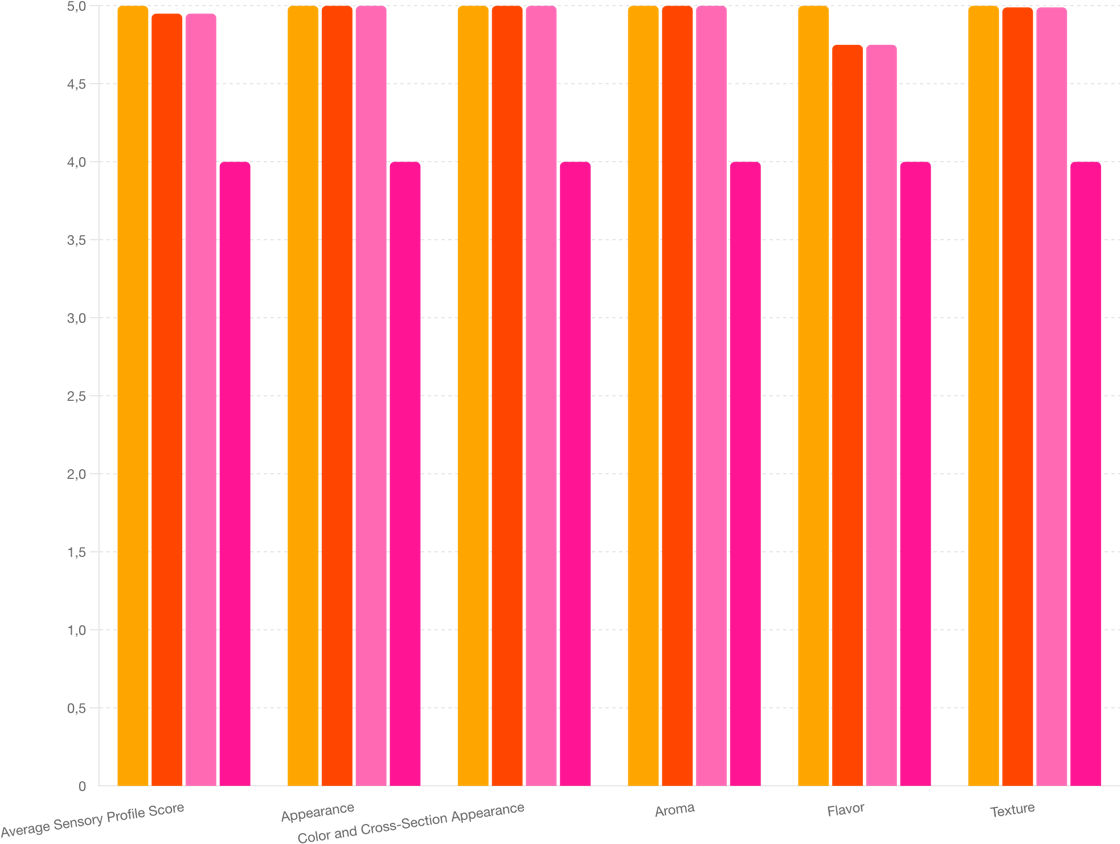
\includegraphics[width=0.8\textwidth]{assets/306}
	\caption*{}
\end{figure}

{\bfseries Figure 1 - Sensory analysis of control and experimental sausage
samples with added purslane}

The control sausage sample received the highest scores across all
parameters (5.00). Samples with 0.8\% and 1.2\% purslane powder also
received high scores, with negligible differences between them: the
average sensory profile score was 4.95 for both samples. According to
the results of the sensory analysis presented in the chart, the
experimental samples 1 and 2 showed no significant differences from the
control in terms of appearance, color, aroma, and flavor, receiving
scores of 5.00, 5.00, 5.00, and 4.75, respectively. The texture was
slightly lower (4.99) but still at a high level. The sample with 1.4\%
purslane showed a significant deterioration in all sensory
characteristics, including the average score (4.00), appearance (4.00),
color (4.00), aroma (4.00), flavor (4.00), and texture (4.00). These
changes are associated with the emergence of a bitter taste and a
greenish tint in the sausage, significantly affecting its appearance.
Given the minimal differences between the samples with 0.8\% and 1.2\%
purslane, we decided to use experiment 2 with a concentration of 1.2\%
as the primary experiment, as it ensures high sensory scores without
significant changes and provides the best physicochemical properties
described above. Thus, adding 1.2\% purslane to sausages maintains their
quality and improves functional characteristics.

Microbiological safety and food quality are key aspects determining
their suitability for consumption. One of the important indicators used
to assess the microbiological quality of food products, including
sausages, is the total viable count (TVC). This indicator allows for
evaluating the total number of microorganisms capable of growing and
forming colonies under aerobic and facultative anaerobic conditions at
moderate temperatures. In the context of growing demand for organic and
natural products, the use of natural additives to improve
microbiological stability and extend the shelf life of food products is
becoming increasingly relevant. Purslane powder (Portulaca oleracea) is
known for its antioxidant and antimicrobial properties, making it a
promising additive for sausages. This study will help determine the
optimal concentration of purslane powder to achieve the best
microbiological indicators without compromising the organoleptic
properties of the product (Table 2).

{\bfseries Table 2 - Study of total viable count (TVC) in experimental
sausage samples}

\begin{longtable}[]{@{}
  >{\raggedright\arraybackslash}p{(\columnwidth - 10\tabcolsep) * \real{0.1668}}
  >{\raggedright\arraybackslash}p{(\columnwidth - 10\tabcolsep) * \real{0.0766}}
  >{\raggedright\arraybackslash}p{(\columnwidth - 10\tabcolsep) * \real{0.1513}}
  >{\raggedright\arraybackslash}p{(\columnwidth - 10\tabcolsep) * \real{0.1968}}
  >{\raggedright\arraybackslash}p{(\columnwidth - 10\tabcolsep) * \real{0.2114}}
  >{\raggedright\arraybackslash}p{(\columnwidth - 10\tabcolsep) * \real{0.1969}}@{}}
\toprule\noalign{}
\begin{minipage}[b]{\linewidth}\raggedright
Parameter
\end{minipage} & \begin{minipage}[b]{\linewidth}\raggedright
Days
\end{minipage} & \begin{minipage}[b]{\linewidth}\raggedright
Control
\end{minipage} & \begin{minipage}[b]{\linewidth}\raggedright
Experiment 1 (0.8\% purslane)
\end{minipage} & \begin{minipage}[b]{\linewidth}\raggedright
Experiment 2 (1.2\% purslane)
\end{minipage} & \begin{minipage}[b]{\linewidth}\raggedright
Experiment 3 (1.4\% purslane)
\end{minipage} \\
\midrule\noalign{}
\endhead
\bottomrule\noalign{}
\endlastfoot
TVC, CFU/g & 1

4

9 & 1,39*10\textsuperscript{2}

1,27*10\textsuperscript{3}

1,43*10\textsuperscript{4} & 1,31*10\textsuperscript{2}

1,47*10\textsuperscript{2}

1,35*10\textsuperscript{3} & 1,11*10\textsuperscript{2}

1,03*10\textsuperscript{2}

1,19*10\textsuperscript{3} & 1,27*10\textsuperscript{2}

1,01*10\textsuperscript{2}

1,05*10\textsuperscript{3} \\
\end{longtable}

On the first day, all samples showed similar initial levels of TVC, with
slight differences. The lowest number of bacteria was recorded in the
sample with 1.2\% purslane (1.11 × 10² CFU/g). After 4 days, the number
of bacteria significantly increased in the control sample (1.27 × 10³
CFU/g). Samples with the addition of purslane demonstrated much lower
bacterial growth. The sample with 1.4\% purslane showed the lowest
number of bacteria (1.01 × 10² CFU/g), indicating a strong antimicrobial
effect. After 9 days, the control sample showed a significant increase
in bacteria (1.43 × 10⁴ CFU/g), whereas the samples with purslane
maintained lower TVC levels. The sample with 1.4\% purslane again
demonstrated the lowest number of bacteria (1.05 × 10³ CFU/g). The
addition of purslane powder to the sausages significantly reduces the
number of viable bacteria compared to the control sample. The lowest
number of bacteria was recorded in samples with 1.2\% and 1.4\%
purslane, especially on days 4 and 9. Experiment 2 (1.2\% purslane) was
chosen as the primary one since it provides a significant reduction in
bacterial load without noticeable deterioration in the sensory
characteristics of the product. In contrast, Experiment 3 (1.4\%
purslane) imparted a bitter taste and a greenish tint to the sausage,
negatively affecting its appearance and flavor.

{\bfseries Conclusion.} This study demonstrated that adding purslane powder
(Portulaca oleracea) to organic sausages significantly improved their
quality and shelf life. The experimental samples with purslane retained
higher moisture levels and exhibited stable pH values, indicating
enhanced product stability. Water activity remained consistent, ensuring
microbiological safety. The total viable count (TVC) was significantly
lower in samples with purslane, especially at 1.2\% and 1.4\%
concentrations, compared to the control. Sensory analysis revealed that
the sample with 1.2\% purslane had high scores similar to the control,
while 1.4\% purslane negatively impacted flavor and appearance. Organic
beef provided a high-quality protein source without synthetic additives,
aligning with consumer demand for healthier products. Purslane powder,
with its antioxidant and antimicrobial properties, proved to be an
effective natural additive. The use of 1.2\% purslane is recommended,
offering a balance between improved quality and sensory attributes. This
natural approach supports the production of high-quality, organic
sausages without synthetic preservatives.

{\bfseries Gratitude, conflict of interest (financing).} This research is
funded by the Ministry of Science and Higher Education of the Republic
of Kazakhstan (BR21882327)

{\bfseries References}

1.Dkhil M.A., Moneim A.E., Al-Quraishy S., Saleh R. Antioxidant effect
of purslane (Portulaca oleracea) and its mechanism of action // Journal
of Medicinal Plants Research. -- 2011. --Vol. 5. --P. 1589-1593.
https://academicjournals.org/journal/JMPR/article-full-text-pdf/C1D5B4017817\#:\textasciitilde:text=Purslane\%20is\%20a\%20potent\%20antioxidant,which\%20act\%20against\%20oxidative\%20stress.

2.Willer H., Lernoud J. The World of Organic Agriculture. Statistics and
Emerging Trends. Research Institute of Organic Agriculture FiBL // IFOAM
Organics International. -2019. ISBN 978-3-03736-119-1

3.Dimitri, C., \& Greene, C. Recent growth patterns in the US organic
foods market // Organic Agriculture. -2016. --Vol. 6(4). --P. 299-310.
DOI 10.22004/ag.econ.33715

4.Esrafil M., Akter S., Alam M., Alim M., Reza M.S., Zubair M.A., Joy
P.R., Jahan M., Khatun M. Development and quality evaluation of novel
biscuits by utilizing fruits and vegetables seed // Food Research.
-2024. --Vol. 8(1). --P. 181-189. DOI 10.26656/fr.2017.8(1).090

5.Das S., Raychaudhuri U., Chakraborty R. Herbal fortification of bread
with fennel seeds // Food Technology and Biotechnology. -2013. --Vol.
51(3). --P. 434-440. https://hrcak.srce.hr/file/160840

6.Petropoulos, S. A., Fernandes, Â., Dias, M. I., Vasilakoglou, I. B.,
Petrotos, K., Barros, L., \& Ferreira, I. C. F. R. Nutritional Value,
Chemical Composition and Cytotoxic Properties of Common Purslane
(Portulaca oleracea L.) // Relation to Harvesting Stage and Plant Part.
In Antioxidants. -2019. --Vol. 8(8). --P. 293-465. DOI
10.3390/antiox8080293

7.Uddin M.K., Juraimi A.S., Hossain M.S., Nahar M.A.A., Ali M.E., Rahman
M.M. (2014). Purslane weed (Portulaca oleracea): a prospective plant
source of nutrition, omega-3 fatty acid, and antioxidant attributes. The
Scientific World Journal, 2014. DOI:10.1155/2014/951019

8. Patarata L., Fernandes L., Silva J.A., Fraqueza M.J. The Risk of Salt
Reduction in Dry-Cured Sausage Assessed by the Influence on Water
Activity and the Survival of Salmonella // Foods. -2022. -Vol.11(30.
-P.444. https://doi.org/10.3390/foods11030444

9. Barbosa-Canovas, G. V., Fontana, A. J., Schmidt, S. J., \& Labuza, T.
P. (Eds.). (2020). Water Activity in Foods: Fundamentals and
Applications/ Wiley.- 616 P. ISBN (electronic)-9781118765982, ISBN
(print- 9781118768316

10.Rashed, A. N., Afifi, F. U., \& Disi, A. M. Simple evaluation of the
wound healing activity of a crude extract of Portulaca oleracea L.
(growing in Jordan) in Mus musculus JVI-1 // Journal of
Ethnopharmacology.-2003.-Vol. 88(2-3).-P. 131-136. DOI:
10.1016/s0378-8741(03)00194-6

\emph{{\bfseries Information about the authors}}

K. Makangali - PhD, Kazakh Agrotechnical Research University named after
S.Seifullin, Astana, Kazakhstan, e-mail: kmakangali@mail.ru;

G. Ospankulova - candidate of biological sciences, Kazakh Agrotechnical
Research University named after S.Seifullin, Astana, Kazakhstan, e-mail:
bulashevag@mail.ru;;

G. Tokysheva - PhD, Kazakh Agrotechnical Research University named after
S.Seifullin, Astana, Kazakhstan, e-mail: tokisheva\_g@mail.ru

\emph{{\bfseries Сведения об авторах}}

Макангали К.К. - PhD, Казахский агротехнический исследовательский
университет им.С.Сейфуллина, Астана, Казахстан, e-mail:
kmakangali@mail.ru

Оспанкулова Г.Х. - к.б.н., Казахский агротехнический исследовательский
университет им.С.Сейфуллина, Астана, Казахстан, e-mail:
bulashevag@mail.ru;

Токышева Г.М. - PhD, Казахский агротехнический исследовательский
университет им.С.Сейфуллина, Астана, Казахстан, e-mail:
tokisheva\_g@mail.ru\newpage
{\bfseries МРНТИ 68.39.49}

СОВРЕМЕННЫЕ ТЕНДЕНЦИИ И АНАЛИЗ ПО ПЕРЕРАБОТКЕ МЯСА КОНИНЫ

В РЕСПУБЛИКЕ КАЗАХСТАН

{\bfseries А.Т. Костанова\textsuperscript{🖂}, Ш.Б. Байтукенова, С.Б.
Байтукенова}

НАО «Казахский агротехнический исследовательский университет им.
С.Сейфуллина»,

Астана, Казахстан,

АО «Казахский университет технологии и бизнеса им. К. Кулажанова»

Астана, Казахстан,

\textsuperscript{🖂}Корреспондент-автор: anel\_kostanova@mail.ru

В данной статье рассмотрены современные тенденции и анализ по
переработке мяса конины в Казахстане. Проведен анализ динамики
численности лошадей во всех категориях. В условиях современного рынка
экономическая эффективность зависит от ряда факторов, в частности, от
рационального применения имеющихся ресурсов, образующих стратегическую
конкурентоспособность отрасли, о чем свидетельствуют высокие результаты
зарубежного использования ресурсов коневодства. В связи с этим были
выявлены внутренние и внешние факторы откорма и переработки мяса,
влияющие на развитие отрасли. В исследовании представлен независимый
всесторонний анализ рынка с использованием различных источников
официальных данных, который отображает текущую ситуацию на рынке
содержания, откорма и переработки конины, оценивает потенциал развития
рынка, рассчитывает все основные ключевые показатели и является хорошим
инструментом для принятия решений при стратегическом планировании и
инвестировании.

Ключевые слова: коневодство, конина, национальная экономика, ресурсы,
развитие рынка.

ҚАЗАҚСТАН РЕСПУБЛИКАСЫНДАҒЫ ЖЫЛҚЫ ЕТІН ӨҢДЕУДЕГІ

ЗАМАНАУИ БАҒЫТТАРЫ МЕН ТАЛДАУЫ

{\bfseries А.Т. Костанова\textsuperscript{🖂}, Ш.Б. Байтукенова, С.Б.
Байтукенова}

«С.Сейфуллин атындағы Қазақ агротехникалық зерттеу университеті» КеАҚ,

Астана қ., Қазақстан,

«Қ.Құлажанов атындағы Қазақ технология және бизнес университеті» АҚ,

Астана қ., Қазақстан,

e-mail: anel\_kostanova@mail.ru

Бұл мақалада Қазақстандағы жылқы ет өңдеу бойынша заманауи үрдістер мен
талдау қарастырылған. Барлық санаттағы жылқылар санының динамикасына
талдау жүргізілді. Қазіргі нарық жағдайында экономикалық тиімділік
бірқатар факторларға, атап айтқанда, саланың стратегиялық бәсекеге
қабілеттілігін құрайтын қолда бар ресурстарды ұтымды пайдалануға
байланысты, бұған жылқы шаруашылығы ресурстарын шетелдік пайдаланудың
жоғары нәтижелері дәлел бола алады. Осыған байланысты саланың дамуына
әсер ететін етті бордақылау мен өңдеудің ішкі және сыртқы факторлары
анықталды. Зерттеу жылқы етін ұстау, бордақылау және қайта өңдеу
нарығындағы ағымдағы жағдайды көрсететін, нарықтың даму әлеуетін
бағалайтын, барлық негізгі көрсеткіштерді есептейтін және стратегиялық
жоспарлау мен инвестициялау кезінде шешім қабылдаудың жақсы құралы болып
табылатын әртүрлі ресми деректер көздерін пайдалана отырып, нарықтың
тәуелсіз жан-жақты талдауын ұсынады.

Түйін сөздер: жылқы шаруашылығы, жылқы еті, ұлттық экономика, ресурстар,
нарықты дамыту.

CURRENT TRENDS AND ANALYSIS OF HORSE MEAT PROCESSING IN THE REPUBLIC OF
KAZAKHSTAN

{\bfseries A.T. Kostanova\textsuperscript{🖂}, Sh.B. Baitukenova, S.B.
Baitukenova}

«S.Seifullin Kazakh Agrotechnical Research University» NJSC,

Astana city, Kazakhstan,

«Kazakh University of Technology and Business named after K.Kulazhanov»
JSC,

Astana city, Kazakhstan,

e-mail: anel\_kostanova@mail.ru

This article discusses current trends and analysis of horse meat
processing in Kazakhstan. The analysis of the dynamics of the number of
horses in all categories was carried out. In the conditions of the
modern market, economic efficiency depends on a number of factors, in
particular, on the rational use of available resources that form the
strategic competitiveness of the industry, as evidenced by the high
results of foreign use of horse breeding resources. In this regard,
internal and external factors of fattening and processing of meat
affecting the development of the industry were identified. The study
presents an independent comprehensive market analysis using various
sources of official data, which reflects the current situation in the
market of horse meat keeping, fattening and processing, assesses the
potential for market development, calculates all the main key indicators
and is a good tool for decision-making in strategic planning and
investment.

Key words: horse breeding, horse meat, national economy, resources;
market development.

Введение. Коневодство разведение лошадей, одна из древнейших отраслей
животноводства. Коневодство как раздел частной зоотехники, базируется на
иппологии. Современное коневодство обладает сведениями по эмбриологии,
популяционной генетике, имууногенетике, полиморфизму ДНК, описаниями
генома лошади, разработаны методы криоконсервации спермы и
трансплантации эмбрионов, методики регуляции
окислительно-восстановительных процессов в организме спортивных лошадей,
управления селекционном процессом в породах.

По данным продовольственной и сельскохозяйственной организации ООН (ФАО)
в мире насчитывается около 60 млн голов лошадей. В настоящее время
конина успешно конкурирует с мясом других видов животных в рационе
населения не только Франции, но и Бельгии, Швеции, Норвегии, Турции,
Дании, Италии, Японии и др. Среди европейских стран Бельгия выделяется
наибольшим потреблением конины на душу населения (в 7-8 раз превышает
потребление баранины). Спрос на мясных лошадей, мороженую и охлажденную
конину на мировом рынке в последние годы систематически растет.
Распределение поголовья лошадей по континентам выглядит следующим
образом: в Азии -- 21,8 млн голов, в Европе -- 7,7 млн голов, в Северной
и Центральной Америке -- 26,1 млн голов, в Африке -- 3,9 млн голов, в
Океании -- 0,5 млн голов (Рисунок 1).

{\bfseries Рис. 1 - Поголовье лошадей по континентам}

Из наиболее перспективных стран в развитии козоводства считаются США (10
млн голов), Китае (7,34 млн голов), Мексике (6,4 млн голов), Бразилии
(6,0 млн голов), Монголоии (4,1 млн голов), Аргентине (2,5 млн голов).
На Американском континенте это такие страны как Мексика, Бразилия,
Аргентина. В Европе -- Балканские страны и страны Средиземноморья
{[}1{]}.

В настоящее время на предприятиях мясной промышленности Казахстана
выпускается разнообразный ассортимент изделий из конины, в том числе
конские вареные мясные продукты и разнообразные национальные изделия.
Видовые особенности конины предопределяют необходимость специального
исследования для интенсификации технологических процессов и улучшения
качества готовой продукции.

Национальная экономика любой страны является сложной хозяйственной,
социальной, организационной и научно-технической системой. В ее основе
исторически сложившаяся структура общественного воспроизводства.

В развитии национальной экономики особую роль играют отрасли
промышленности. Отрасль промышленности является комплексом предприятий,
который имеют однотипное экономическое назначение производимой
продукции, общую техническую базу, особый профессиональный состав
работников, специфику работы, используют однородные потребляемые
материалы и характеризуются однотипностью технологических процессов.
Иными словами, отрасль промышленности объединяет предприятия, которые
производят однородную продукцию, используют похожие технологии и имеют
свой круг потребителей.

Анализ состояния перерабатывающей промышленности в рамках исследования
был проведен на примере мясной отрасли. Мясная промышленность -- отрасль
пищевой промышленности, перерабатывающая скот. По данным агентства
статистики Министерства национальной экономики Республики Казахстан по
состоянию на 1 июня 2023 года в Казахстане распределение численности
скота в Казахстане: овец -- 25, 9 млн голов (57\%); крупного рогатого
скота -- 10,5 млн голов (23\%); лошадей -- 4,5 млн голов (10\%); коз --
3,2 млн голов (7\%); верблюдов -- 292 тыс.голов (1\%) (Рисунок 2)
{[}2{]}.

\begin{figure}[H]
	\centering
	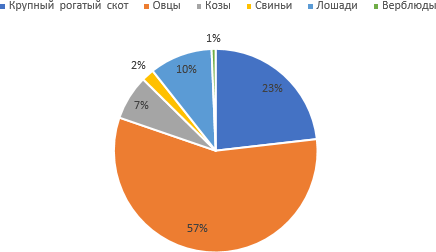
\includegraphics[width=0.8\textwidth]{assets/307}
	\caption*{}
\end{figure}

Рис. 2 - Численность скота по состоянию на 1 июня 2023 г. в Казахстане

Современная экономика Казахстана ведет свой отсчет с 1991 года, когда
произошел распад СССР. С этого момента страна взяла курс на модернизацию
экономики, а также на интеграцию в экономическое пространство. В
Казахстане плановая рыночная модель экономики, которая в настоящее время
интенсивно развивается. Казахстан активно наращивает собственное
производство, прежде всего, развивая пищевую промышленность, в частности
мясную промышленность. Эта отрасль крайне важна, поскольку связана с
производством сырья, материалов и продуктов, направленных на
удовлетворение пищевых потребностей населения. Согласно динамике объема
рынка конины в Казахстане в период 1991-2022 гг.: наибольшая прибавка
поголовья лошадей в Казахстане наблюдается в 1999 г. -- 127,2 тыс.
голов, 2011 г. -- 121,5, 1992 г. -- 121,4 тыс.голов (Рисунок 3).

\begin{figure}[H]
	\centering
	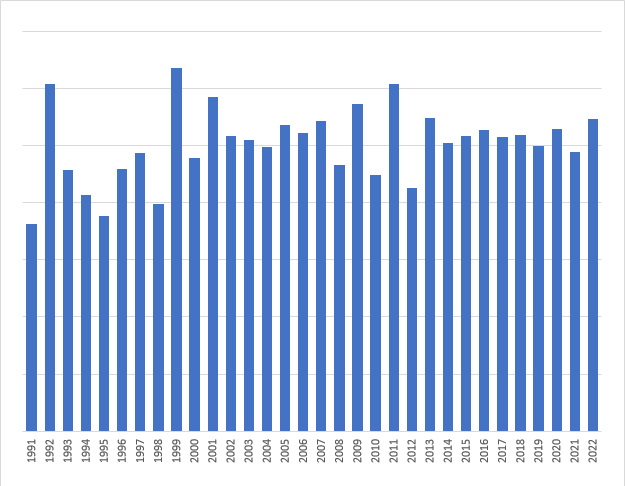
\includegraphics[width=0.8\textwidth]{assets/308}
	\caption*{}
\end{figure}

Рис. 3 - Динамика объема рынка конины в Казахстане в 1991-2022 гг.,
тыс.голов

Коневодство в Казахстане -- это важный вид деятельности в сельском
хозяйстве, которая в последнее время интенсивно развивается. Благодаря
особенным климатическим условиям, огромными запасами воды и большими
пастбищными хозяйствами, Акмолинская область является подходящей для
разведения лошадей. В 2023 году поголовье лошадей в областях составляло
4,5 млн голов, в том числе в сельскохозяйственных предприятиях 299 тыс.
голов (6,7 \%), у населения 1,9 млн голов (42,2 \%), в крестьянских
(фермерских) хозяйствах и у индивидуальных предпринимателей - 2,3 млн
голов (51,1 \%) {[}3{]}.

Казахстан входит в первую десятку стран мира с наиболее развитым
коневодством. В силу обширности территории, сложных дорожных условий,
многообразия природно-климатических зон и национальных традиций
использование лошадей в Казахстане остается многоплановым. Разводят
свыше 40 пород, по данным СтатБюро (2023), общее поголовье составляет
1,303 млн, из них около 30\% - продуктивные животные, около 4,5\% -
племенные и спортивные, остальные -- рабоче-пользовательные. Основное
пооголовье находится во владении акционерных обществ, кооперативов,
товариществ, фермерских и подсобных хозяйств. В структуре племенного
коневодства действуют около 100 конных заводов, около 300 племенных
ферм, государственные заводские конюшни и др. Всего насчитывается 1500
предприятий по разведению лошадей. Возрастают потребности в конине и
кумысе, расширяется ареал продуктивного коневодства. Стабильно
востребовано рабоче-пользовательное коневодство. Научно-обоснованная
потребность в поголовье лошадей всех направлений использования в
Казахстане -- свыше 6,2 млн голов {[}4{]}.

\begin{figure}[H]
	\centering
	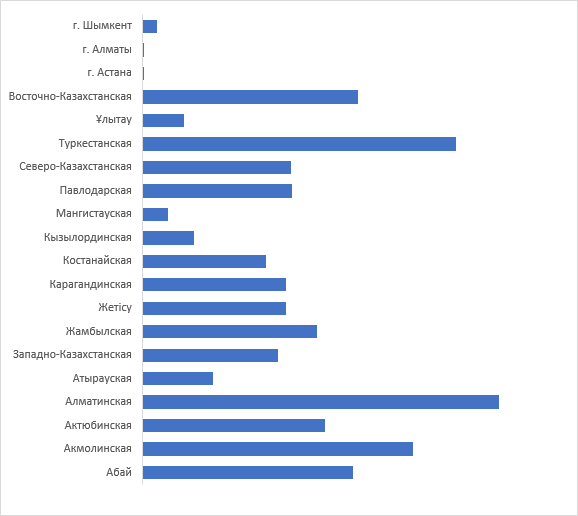
\includegraphics[width=0.8\textwidth]{assets/309}
	\caption*{}
\end{figure}

Рис. 4 - Численность поголовья лошадей по состоянию на 1 июня

по Республике Казахстан, голов

Наибольшая прибавка поголовья лошадей в Казахстане наблюдается в двух
регионах: Алматинская -- 221,5 тыс. голов; Туркестанская -- 194,8 тыс.
голов (Рисунок 4).

{\bfseries Материалы и методы.} ГОСТ 32225-2013 Лошади для убоя~Конина и
жеребятина в полутушах и четвертинах. Технические условия. Horses for
slaughter. Horseflesh in semi-carcasses and quarters. Specifications
{[}5{]}.

ГОСТ 27095-86 Конина и жеребятина в полутушах и четвертинах Технические
условия. Meat. Horse meat and young horse meat in half-carcasses and
quarters.~\\
Specifications {[}6{]}.

Результаты и обсуждение. В продовольственной программе Казахстана
большое внимание уделяется развитию мясной промышленности. Поставлена
задача увеличить мясные ресурсы за счет развития скотоводства, в том
числе и коневодства.

Конина издавна имеет большое значение в питании населения Казахстана,
Кыргызстане, Якутии, Бурятии, Узбекистане, Татарстане, Башкортостане.
Она является одним из ценных видов мяса, так как более богата белками,
чем говядина и свинина.

Крупной базой коневодства является Казахстан. По численности поголовья
лошадей она занимает второе место среди бывших союзных республик. В
Казахстане продуктивное коневодство сложилось в самостоятельную отрасль
животноводства, перед которой поставлена задача -- удовлетворить
потребности населения в высококачественной конине. Здесь имеются
благоприятные условия для развития мясного коневодства.

Ароматное нежное мясо молодых лошадей считается ценным сырьем для
изготовления национальных изделий.

Резервы увеличения производства конины следующие: рост поголовья лошадей
в селах самостоятельной отрасли мясного коневодства, правильная
организация кормовой базы, кормление, нагулы, откорм и разведение
лошадей, сдаваемых на мясо, и х доращивание, борьба с потерями поголовья
скота, а также с потерями его упитанности при транспортировке на
предприятия.

Рост поголовья в коневодстве за последние пять лет составил 45,8\%, что
делает отрасль лидером в мясном и племенном животноводстве. Коневодство
по сравнению с другими направлениями животноводства ниже, а продукция
имеет устойчивый спрос и высокую маржинальную прибыль, поскольку
сбывается по цене выше говядины и баранины. Так, в ноябре 2023 г. цена
килограмма говядины в Казахстане составляла в среднем от 2,5 тыс. тенге
до 3,5 тыс. тенге в разных регионах страны, а баранины -- от 1,8 до 2,3
тыс. тенге. Конина же сбывалась в ценовом диапазоне от 1,8 до 3,5 тыс.
тенге за кг, и это при себестоимости в 400-500 тенге. Низкая
себестоимость производства конины обусловлена тем, что лошадей можно
пасти круглый год. Но при этом из-за более высоких вкусовых качеств и
традиций в Казахстане конина будет дороже и говядины, и баранины.

Согласно данным статистического бюро, потребление в Казахстане говядины
составило во втором квартале 2023 г. 5,6 кг на одного жителя страны, а
баранины -- 1,7 кг за тот же период. Это пока превышает потребление
конины - 1 кг.

При этом конина 2023 г. дорожала медленнее, чем два ее основных
конкурента по внутреннему рынку -- 13 \% рост в цене за 10 месяцев
против 15\% роста стоимости говядины за тот же период и 15,6\% роста
цены баранины {[}7{]}.

Популярность лошадиного мяса на рынке постепенно растет. Причиной тому
выступает состав продукта. Мясо является отличным источником белка. Как
объяснялось выше, эти белки выполняют определенные функции в живой
мышечной ткани и при преобразовании мышц в мясо. К ним относятся актин и
миозин (миофибриллярные белки), гликолитические ферменты и миоглобин
(саркоплазматические белки) и коллаген (белки соединительной ткани).
Поскольку белки, содержащиеся в мясе, обеспечивают рацион всеми девятью
незаменимыми аминокислотами, мясо считается полноценным источником
белка. Включает протеин -- не менее 15--20\%; воду -- 70\%; жиры в
количестве 2--5\%; золу -- около 1\%. Что касается микроэлементов, то в
составе конины основную часть занимают: калий, железо, натрий, фосфор и
др. Богата конина и на витамины. Такой состав предполагает высокую
энергетическую ценность продукта. По своей калорийности он относится к
числу среднекалорийных и составляет около 120-180 ккал на каждые 100 г
мяса. Диетологи утверждают, что конина рекомендована детям в качестве
первого прикорма, особенно страдающим аллергией {[}8{]}.

В рационе жиры, содержащиеся в мясе, служат переносчиками
жирорастворимых витаминов (А, D, Е и К) и поставляют необходимые
вещества не поставляемые организмом). Помимо своей роли запаса энергии,
жирные кислоты являются предшественниками в синтезе. Жирнокислотный
состав мяса зависит от нескольких факторов. Рацион питания лошадей при
откорме может существенно изменить состав жирных кислот мяса. Если
кормить добавками с высоким содержанием ненасыщенных жиров, жир, который
они откладывают в мышцах, будет иметь повышенный уровень ненасыщенных
жирных кислот. При классификации мяса мясо разделяется на разные классы
на основе ожидаемых пищевых качеств (например, внешнего вида, нежности,
сочности и вкуса) и ожидаемого выхода товарного мяса из тушки. В отличие
от процедур проверки мяса, системы классификации мяса значительно
различаются во всем мире. Эти различия во многом обусловлены тем, что в
разных странах действуют разные стандарты качества мяса. Например, в
Соединенные Штаты скот откармливают в первую очередь для производства
стейков и откармливают высококачественными зерновыми кормами для
достижения высокого количества по всей мускулатуре животного. Высокий
уровень качества мяса связан с более сочными, более ароматными и нежными
комбикормами при откорме {[}9{]}. Самым распространенным компонентом
мяса является -- вода. Однако, поскольку жировая ткань содержит мало
влаги или вообще не содержит ее, по мере увеличения процента жира в
куске мяса процент воды снижается. Таким образом, нежирная молодая
конина может содержать до 80 процентов воды, а полностью откормленная
конина --- до 50 процентов. Поскольку при приготовлении мяса теряется
вода, процентное содержание белка и жира в приготовленном мясе обычно
выше, чем в сыром.

На содержание миоглобина в скелетных мышцах влияет ряд факторов
кормления и процесса убоя. Мышцы представляют собой смесь двух разных
типов мышечных волокон: быстро сокращающихся и медленно сокращающихся,
пропорции которых различаются между мышцами. Быстро сокращающиеся
волокна имеют низкое содержание миоглобина, поэтому их еще называют
белые волокна. Медленно сокращающиеся волокна содержат большое
количество миоглобина и обладают большей способностью к окислительному
метаболизму. Эти волокна часто называют красные волокна. Следовательно,
темный цвет мяса является результатом относительно высокой концентрации
медленно сокращающихся волокон в мышцах животного. При составлении
перспективных планов содержания и откорма животных, на примере
производства конины, широко используются различные нормативы.
Применительно к табунному коневодству в экономической и
сельскохозяйственной литературе для отдельных регионов страны также
разрабатывались нормативные показатели рациона питания {[}10{]}.
Республика Казахстан с наличием огромных территорий естественных пастбищ
(180 млн га) имеет значительные перспективы в снабжении страны
экологически чистыми продуктами питания. Крупным резервом выполнения
Продовольственной программы республики является отгонное животноводство,
в частности, коневодство. Необходимо отметить, что на протяжении
последнего десятилетия государство приняло ряд программ, направленных на
развитие агропромышленного комплекса страны {[}11{]}.

Для обеспечения качества мясных продуктов из конины, необходимо
оптимизировать выход конечной продукции по всей цепочке создания
стоимости. Одним из факторов влияющих на повышение эффективности всей
цепочки создания стоимости является комплекс использования оборудования
для переработки. Начиная с конкретных процессов, таких как взвешивание,
нарезка и маркировка, до комплексных решений, таких как линии обвалки,
обрезки, приготовления мяса, нарезки на порции и формовки
мясопереработки с постоянным вниманием к гигиене и безопасности.
Количество оборудования будет зависеть от используемых процедур убоя и
переработки.

{\bfseries Выводы.} В настоящее время в Казахстане пищевая промышленность
развивается достаточно сбалансированно. Мясная отрасль нуждается в
разработке новых методов откорма с применением инновационных
информационно-технических решений и привлечении инвестиций для оснащения
высокопроизводительным оборудованием для переработки с целью обеспечения
повышения эффективности производства конины.

Повышение экономической эффективности позволит сделать коневодство одним
из рентабельных направлений животноводства, обеспечивающим необходимый
ресурс для устойчивого животноводства и удовлетворяющим растущий спрос
на белок в пище для быстро растущего населения.

Литература

1. Продовольственная и сельскохозяйственная организация Объединенных
наций URL: http://www.fao.org/home/ru/ {[}Электронный ресурс{]}. (дата
обращения - 12.03.2024)

2. Данные Комитета по статистике Министерства национальной экономики
Республики Казахстан по состоянию на январь-октябрь 2023 года. -URL:
https://www.gov.kz/memleket/entities/economy?lang=ru {[}Электронный
ресурс{]}. (дата обращения 12.03.2024)

3. Бюро национальной статистики агентства по стратегическому
планированию и реформам Республики Казахстан по состоянию на 1 июня 2023
года. - URL: https://stat.gov.kz/ru/ {[}Электронный ресурс{]}. Дата
обращения - 12.03.2024

4. Большая Российская энциклопедия. - URL:
https://bigenc.ru/c/konevodstvo-394ab0 {[}Электронный ресурс{]}. Дата
обращения - 12.03.2024

5. ГОСТ 32225-2013. Лошади для убоя~Конина и жеребятина в полутушах и
четвертинах. Технические условия. Horses for slaughter. Horseflesh in
semi-carcasses and quarters. Specifications. -- Взамен ГОСТ 20079-74;
введ - 01.07.2015. --Москва: Межгосударственный стандарт. - М.: Изд-во
стандартов, 2015.

6. ГОСТ 27095-86. Конина и жеребятина в полутушах и четвертинах.
Технические условия. Meat. Horse meat and young horse meat in
half-carcasses and quarters.~\\
Specifications. - Взамен ГОСТ 20079-74; введ -- 01.01.1988. --Москва:
Межгосударственный стандарт. - М. : Изд-во стандартов, 2006.

7. Бас аграрлық сайт URL: https://eldala.kz {[}Электронный ресурс{]}.
(дата обращения - 12.03.2024)

8. Инербаева А.Т. Производители конины и ее переработка на качественные
мясные продукты.//Сибирский научно-исследовательский и технологический
институт переработки сельскохозяйственной продукции Сибирского
Федерального научного центра агробиотехнологий Российской академии наук
(СибНИТИП СФНЦА РАН).- Материалы

международной научно-практической конференции, посвященной 100-летию
доктора cельскохозяйственных наук, профессора, заслуженного деятеля
науки Российской Федерации и Республики Бурятия Мункоева Константина
Тармаевича. - Новосибирск, Россия. - 2019. -с.103-109

9. The American Association of Meat Processors (AAMP). --URL:
https://www.aamp.com/ (date of application - 03/12/2024)

10. Нурушева Г.М. Научное обоснование эффективности продуктивного
коневодства на Севере Казахстана // Известия Оренбургского
государственного аграрного университета, -2011. -№. 4(32-1). -С.
247-249.

11. Есенгалиева С.М., Мансурова М.А., Махмудов А.Д., Федорченко Л.В.
Современное состояние и тенденции развития животноводства в Республике
Казахстан.~~Economics: the strategy and practice. -2021. №16(2).
-P134-144. DOI 10.51176/1997-9967-2021-2-134-144.

References

1. Prodovol\textquotesingle stvennaya i
sel\textquotesingle skokhozyaistvennaya organizatsiya Ob"edinennykh
natsii URL: http://www.fao.org/home/ru/ {[}Elektronnyĭ resurs{]}. (data
obrashcheniya - 12.03.2024) {[}in Russian{]}

2. Dannye Komiteta po statistike Ministerstva
natsional\textquotesingle noĭ ekonomiki Respubliki Kazakhstan po
sostoyaniyu na yanvar\textquotesingle-oktyabr\textquotesingle{} 2023
goda. -URL: https://www.gov.kz/memleket/entities/economy?lang=ru
{[}Elektronnyĭ resurs{]}. (data obrashcheniya 12.03.2024) {[}in
Russian{]}

3. Byuro natsional\textquotesingle noi statistiki agentstva po
strategicheskomu planirovaniyu i reformam Respubliki Kazakhstan po
sostoyaniyu na 1 iyunya 2023 goda. - URL: https://stat.gov.kz/ru/
{[}Elektronnyĭ resurs{]}. Data obrashcheniya - 12.03.2024 {[}in
Russian{]}

4. Bol\textquotesingle shaya Rossiiskaya entsiklopediya. - URL:
https://bigenc.ru/c/konevodstvo-394ab0 {[}Elektronnyĭ resurs{]}. Data
obrashcheniya - 12.03.2024 {[}in Russian{]}

5. GOST 32225-2013. Loshadi dlya uboya Konina i zherebyatina v
polutushakh i chetvertinakh. Tekhnicheskie usloviya. Horses for
slaughter. Horseflesh in semi-carcasses and quarters. Specifications. --
Vzamen GOST 20079-74; vved - 01.07.2015. --Moskva: Mezhgosudarstvennyi
standart. - M.: Izd-vo standartov, 2015. {[}in Russian{]}

6. GOST 27095-86. Konina i zherebyatina v polutushakh i chetvertinakh.
Tekhnicheskie usloviya. Meat. Horse meat and young horse meat in
half-carcasses and quarters.

Specifications. - Vzamen GOST 20079-74; vved -- 01.01.1988. --Moskva:
Mezhgosudarstvennyi standart. - M. : Izd-vo standartov, 2006. {[}in
Russian{]}

7. Bas agrarlyq sait URL: https://eldala.kz {[}Elektronnyĭ resurs{]}.
(data obrashcheniya - 12.03.2024) {[}in Russian{]}

8. Inerbaeva A.T. Proizvoditeli koniny i ee pererabotka na kachestvennye
myasnye produkty.//Sibirskii nauchno-issledovatel\textquotesingle skii i
tekhnologicheskii institut pererabotki
sel\textquotesingle skokhozyaistvennoi produktsii Sibirskogo
Federal\textquotesingle nogo nauchnogo tsentra agrobiotekhnologii
Rossiiskoi akademii nauk (SibNITIP SFNTsA RAN), materialy mezhdunarodnoi
nauchno-prakticheskoi konferentsii, posvyashchennoi 100-letiyu doktora
cel\textquotesingle skokhozyaistvennykh nauk, professora, zasluzhennogo
deyatelya nauki Rossiiskoi Federatsii i Respubliki Buryatiya Munkoeva
Konstantina Tarmaevicha. - Novosibirsk, Rossiya. - 2019. -S.103-109
{[}in Russian{]}

9. The American Association of Meat Processors (AAMP). --URL:
https://www.aamp.com/ (date of application - 03/12/2024)

10. Nurusheva G.M. Nauchnoe obosnovanie effektivnosti produktivnogo
konevodstva na Severe Kazakhstana // Izvestiya Orenburgskogo
gosudarstvennogo agrarnogo universiteta, -2011. -№. 4(32-1). -S.
247-249. {[}in Russian{]}

11. Esengalieva S.M., Mansurova M.A., Makhmudov A.D., Fedorchenko L.V.
Sovremennoe sostoyanie i tendentsii razvitiya zhivotnovodstva v
Respublike Kazakhstan. Economics: the strategy and practice. -2021.
№16(2). -P134-144. DOI 10.51176/1997-9967-2021-2-134-144. {[}in
Russian{]}

\emph{Сведения об авторах}

Анель Т.К. - докторант НАО «Казахский агротехнический исследовательский
университет им. С.Сейфуллина», Астана, Казахстан, e-mail:
anel\_kostanova@mail.ru;

Шолпан Б.Б. - кандидат технических наук, и.о. ассоциированного
профессора НАО «Казахский агротехнический исследовательский университет
им. С.Сейфуллина», Астана, Казахстан, e-mail: baytukenova75@mail.ru;

Сауле Б.Б. - кандидат технических наук, и.о. ассоциированного профессора
АО «Казахский университет технологии и бизнеса им. К. Кулажанова»,
Астана, Казахстан, e-mail: saule7272@mail.ru

\emph{Information about the authors}

Anel T.K. - PhD student «S.Seifullin Kazakh Agrotechnical Research
University» NJSC, Astana, Kazakhstan, e-mail: anel\_kostanova@mail.ru;

Sholpan B.B. -- candidate of technical sciences, acting associate
professor «S.Seifullin Kazakh Agrotechnical Research University» NJSC,
Astana, Kazakhstan, e-mail: baytukenova75@mail.ru;

Saule B.B. -- candidate of technical sciences, acting associate
professor «Kazakh University of Technology and Business named after
K.Kulazhanov» JSC, Astana, Kazakhstan, e-mail: saule7272@mail.ru

.\newpage
{\bfseries МРНТИ 65.09.05}; 65.13.13

{\bfseries УСТАНОВКА ДЛЯ КАПСУЛИРОВАНИЯ ПРОБИОТИКОВ}

{\bfseries \textsuperscript{1}М.М. Ташыбаева\textsuperscript{🖂},
\textsuperscript{1}А.К. Какимов, \textsuperscript{2}А.А. Майоров,
\textsuperscript{1}Г.А. Жумадилова}

\textsuperscript{1} НАО Университет им. Шaкapимa гopoдa Ceмeй ,
Казахстан, Семей,

\textsuperscript{2} ФГБНУ Федеральный Алтайский научный центр
агробиотехнологий,

Барнаул, Россия

{\bfseries \textsuperscript{🖂}}Корреспондент-автор:
marzhan06081990@gmail.com

Инкапсуляция является весьма актуальным процессом на сегодняшний день,
так как позволяет защитить инкапсулируемый материал (пробиотик) от
воздействий окружающей среды: влага, тепло и т.д., тем самым повышая
шансы на выжимаемость. Для подбора оптимального процентного соотношения
альгината натрия 0,5\%, 0,8\%, 1\%. Эксперименты проводились при
температурах гелеобразующей смеси от 20 до 50 ℃. Была выбрана форсунка с
выходным отверстием d= 1,2×10\textsuperscript{-3}м, как наиболее
оптимальная и по производительности, и по качесту получаемых капсул. При
определении вязкости в вискозиметре Брукфильда постоянный режим выходит
после частоты вращения ротора от 0,333 с\textsuperscript{-1} до 0,833
с\textsuperscript{-1}. В полученную смесь внесли навеску штамма
пропионовокислых бактерий Propionibacterium freudenreichii. В конечном
итоге, получили округлые капсулы, содержащие пробиотик Propionibacterium
freudenreichii, которые могут быть использованы в дальнейших
технологических процессах при получении пищевых продуктов
лечебно-профилактического действия или при получении фармокологических
препаратов. Гелеобразное сырье при нагнетании давления с помощью
шестеренчатого насоса испытывает мгновенно-упругую деформацию и в
дальнейшем, при напряжении превышающем предел текучести,
вязкопластическую деформацию. Под действием давления и испытываемых
деформаций, гелеобразное сырье попадает в форсунку, разбрызгивается, в
дальнейшем образует микрокапсулы.

{\bfseries Ключевые слова:} микрокапсула, пробиотик, шестеренчатый насос,
форсунка, альгинат, распылительный метод

{\bfseries INSTALLATION FOR CAPSULIATION OF PROBIOTICS}

{\bfseries \textsuperscript{1}M.М. Tashybayeva\textsuperscript{🖂},
\textsuperscript{1}A.К. Kakimov, \textsuperscript{2}A.А. Mayorov,
\textsuperscript{1}G.А. Zhumadilova}

\textsuperscript{1}NJSC Shakarim University of Semey , Semey,
Kazakhstan,

\textsuperscript{2}Federal State Budget Scientific Institution Federal
Altai Scientific Center for Agrobiotechnologies , Barnaul, Russian,

e-mail: marzhan06081990@gmail.com

Encapsulation is a very relevant process today, as it allows you to
protect the encapsulated material (probiotic) from environmental
influences: moisture, heat, etc., thereby increasing the chances of
squeezability. To select the optimal percentage of sodium alginate
0.5\%, 0.8\%, 1\%. The experiments were carried out at temperatures of
the gel-forming mixture from 20 to 50 ℃. A nozzle with an outlet hole d=
1,2×10\textsuperscript{-3}м was selected as the most optimal both in
terms of performance and quality of the capsules obtained. When
determining the viscosity in the Brookfield viscometer, the constant
mode goes out after the rotor speed from 0,333 с\textsuperscript{-1} до
0,833 с\textsuperscript{-1}. A suspension of a strain of propionic acid
bacteria Propionibacterium freudenreichii was added to the resulting
mixture. Eventually, rounded capsules containing the probiotic
Propionibacterium freudenreichii were obtained, which can be used in
further technological processes in the production of food products of
therapeutic and preventive action or in the production of
pharmacological preparations. The gellike raw material, when pressurized
with a gear pump, experiences instantaneous elastic deformation and
further, at a stress exceeding the yield strength, viscoplastic
deformation. Under the influence of pressure and the deformations
tested, the gellike raw material enters the nozzle, is sprayed, and then
forms microcapsules.

{\bfseries Key words:} microcapsule, probiotic, gear pump, nozzle,
alginate, spray method

{\bfseries ПРОБИОТИКТЕРДІ КАПСУЛАЛАУҒА АРНАЛҒАН ҚОНДЫРҒЫ}

{\bfseries М.М. Ташыбаева\textsuperscript{🖂}, \textsuperscript{1}А.К.
Какимов, \textsuperscript{2}А.А. Майоров, \textsuperscript{1}Г.А.
Жумадилова}

\textsuperscript{1}Семей қаласының Шәкәрім атындағы университеті КеАҚ,
Ceмeй, Қазақстан

Федералдық Алтай агробиотехнологиялық ғылыми орталығы ФМБҒМ,

Барнаул, Ресей,

e-mail: marzhan06081990@gmail.com

Капсулалау бүгінгі күні өте өзекті процесс, өйткені ол капсулаланған
материалды (пробиотикті) қоршаған орта әсерінен: ылғалдан, жылудан және
т.б. қорғауға мүмкіндік береді, осылайша сығу мүмкіндігін арттырады.
Натрий альгинатының оңтайлы пайызын таңдау үшін 0,5\%, 0,8\%, 1\%
алынды. Тәжірибелер гель түзетін қоспаның 20-дан 50 ℃-ге дейін
температурасында жүргізілді. Өнімділік жағынан да, алынған капсулалардың
сапасы бойынша да ең оңтайлы ретінде диаметрі d= 1,2×10
\textsuperscript{-3}м форсунка таңдалды. Брукфильд вискозиметріндегі
тұтқырлықты анықтау кезінде тұрақты режим ротордың 0,333
с\textsuperscript{-1} және 0,833 с\textsuperscript{-1} дейін айналу
жиілігінен кейін шығады. Алынған қоспаға Propionibacterium
freudenreichii пропион қышқылы бактерияларының штаммы қосылды. Соңында
біз пробиотикалық Propionibacterium freudenreichii бар дөңгелек
капсулаларды алдық, оларды емдік-профилактикалық әсері бар тамақ
өнімдерін өндіру немесе фармакологиялық препараттарды өндіру үшін одан
әрі технологиялық процестерде қолдануға болады. Гель тәрізді шикізат
беріліс сорғысының көмегімен қысымды айдау кезінде лезде серпімді
деформацияны және одан әрі, аққыштық шегінен асатын кернеуде тұтқыр
пластикалық деформацияны сезінеді. Қысым мен сыналған деформациялардың
әсерінен гель тәрізді шикізат форсункаға түседі, шашырайды, әрі қарай
микрокапсулалар түзеді.

{\bfseries Түйін сөздер:} микрокапсула, пробиотик, тісті сорғы, форсунка,
альгинат, шашырату әдісі

{\bfseries Введение.} Здоровье человека, как и качество его жизни во многом
определяется качеством потребляемой пищи. Пища должна содержать все
необходимые вещества для нормального функционирования организма
человека. В наше время большое количество людей из-за
несбалансированного питания, малоподвижного образа жизни и нарушенного
режима страдают болезнями желудочно-кишечного тракта {[}1{]}.

В последнее время в целях повышения и поддержания иммунитета человека,
широко применяют пробиотики, так как они благотворно влияют на
микрофлору человека. Пробиотики улучшают пищеварение, повышают
устойчивость к инфекционным заболеваниям и проявляют терапевтический
эффект при острых кишечных инфекциях. Благотворное влияние пробиотиков
на организм человека определяется положительными свойствами
микроорганизмов, входящих в состав пробиотиков. В основном, состав
пробиотиков включает представителей эндогенной флоры кишечника:
бифидобактерии, кишечную палочку, энтерококков, лактобактерии и др. Они
вносят существенный вклад в нормальное функционирование организма.
Заключение биологически активных добавок, ферментов, клеток и др.
материалов в мелкие капсулы называется процессом инкапсулирования.
Инкапсуляция является весьма актуальным процессом на сегодняшний день,
так как позволяет защитить инкапсулируемый материал (пробиотик) от
воздействий окружающей среды: влага, тепло и т.д., тем самым повышая
шансы на выжимаемость {[}1, с.8{]}.

В пищевой промышленности инкапсуляцию используют для скрытия запахов и
вкусовых качеств {[}2{]}. При употреблении живых микроорганизмов -
пробиотиков, организм человека начинает лучше функционировать {[}3{]}.

Инкапсулирование позволит сохранить жизнеспособность пробиотиков, что
является важным аспектом для оптимальной работы желудочно-кишечного
тракта {[}4{]}.

Альгинат - природный полисахарид (лат. Phaeophyceae, ламинария японская
(лат. Laminaria Japonica Aresch). Содержание альгиновой кислоты в
ламинарии составляет от 15 до 30\%) и бактерии.

Альгинатные гидрогели для капсулирования клеток широко используются
{[}5; 6{]}, а альгинат кальция подходит для инкапсуляции пробиотиков
из-за простоты использования, не токсичности, биодоступности и низкой
стоимости {[}7; 8; 9{]}.

Биологические, химические и физические свойства капсулированных
функциональных продуктов определяются технологиями и оборудованием,
используемыми для их производства. Существует множество методов
получения капсулированных функциональных продуктов, однако, немаловажным
фактором при выборе технологии производства, является экономичность
производственного процесса, простота эксплуатации, более низкая
себестоимость конечного продукта при сохранении всех необходимых
терапевтических, органолептических, функциональных качеств.

Способы получения капсул вручную, капельным методом, распылительным
методом широко применяются на сегодняшний день, но данный процесс
является очень трудоемким и долгим, соответственно, низкоэффективным и
затратным.

На основании вышесказанного, была поставлена задача усовершенствования
установки для получения функциональных капсул продукта (в частности
пробиотиков), что позволяет автоматизировать процесс получения капсул с
пробиотиками.

Цель работы капсулирование пробиотиков методом распыления с
усовершенствованной установкой для капсулирования.

{\bfseries Методы исследования.} Установка для капсулирования пробиотиков
показана на рисунке 1 {[}10; 11{]}.

\begin{figure}[H]
	\centering
	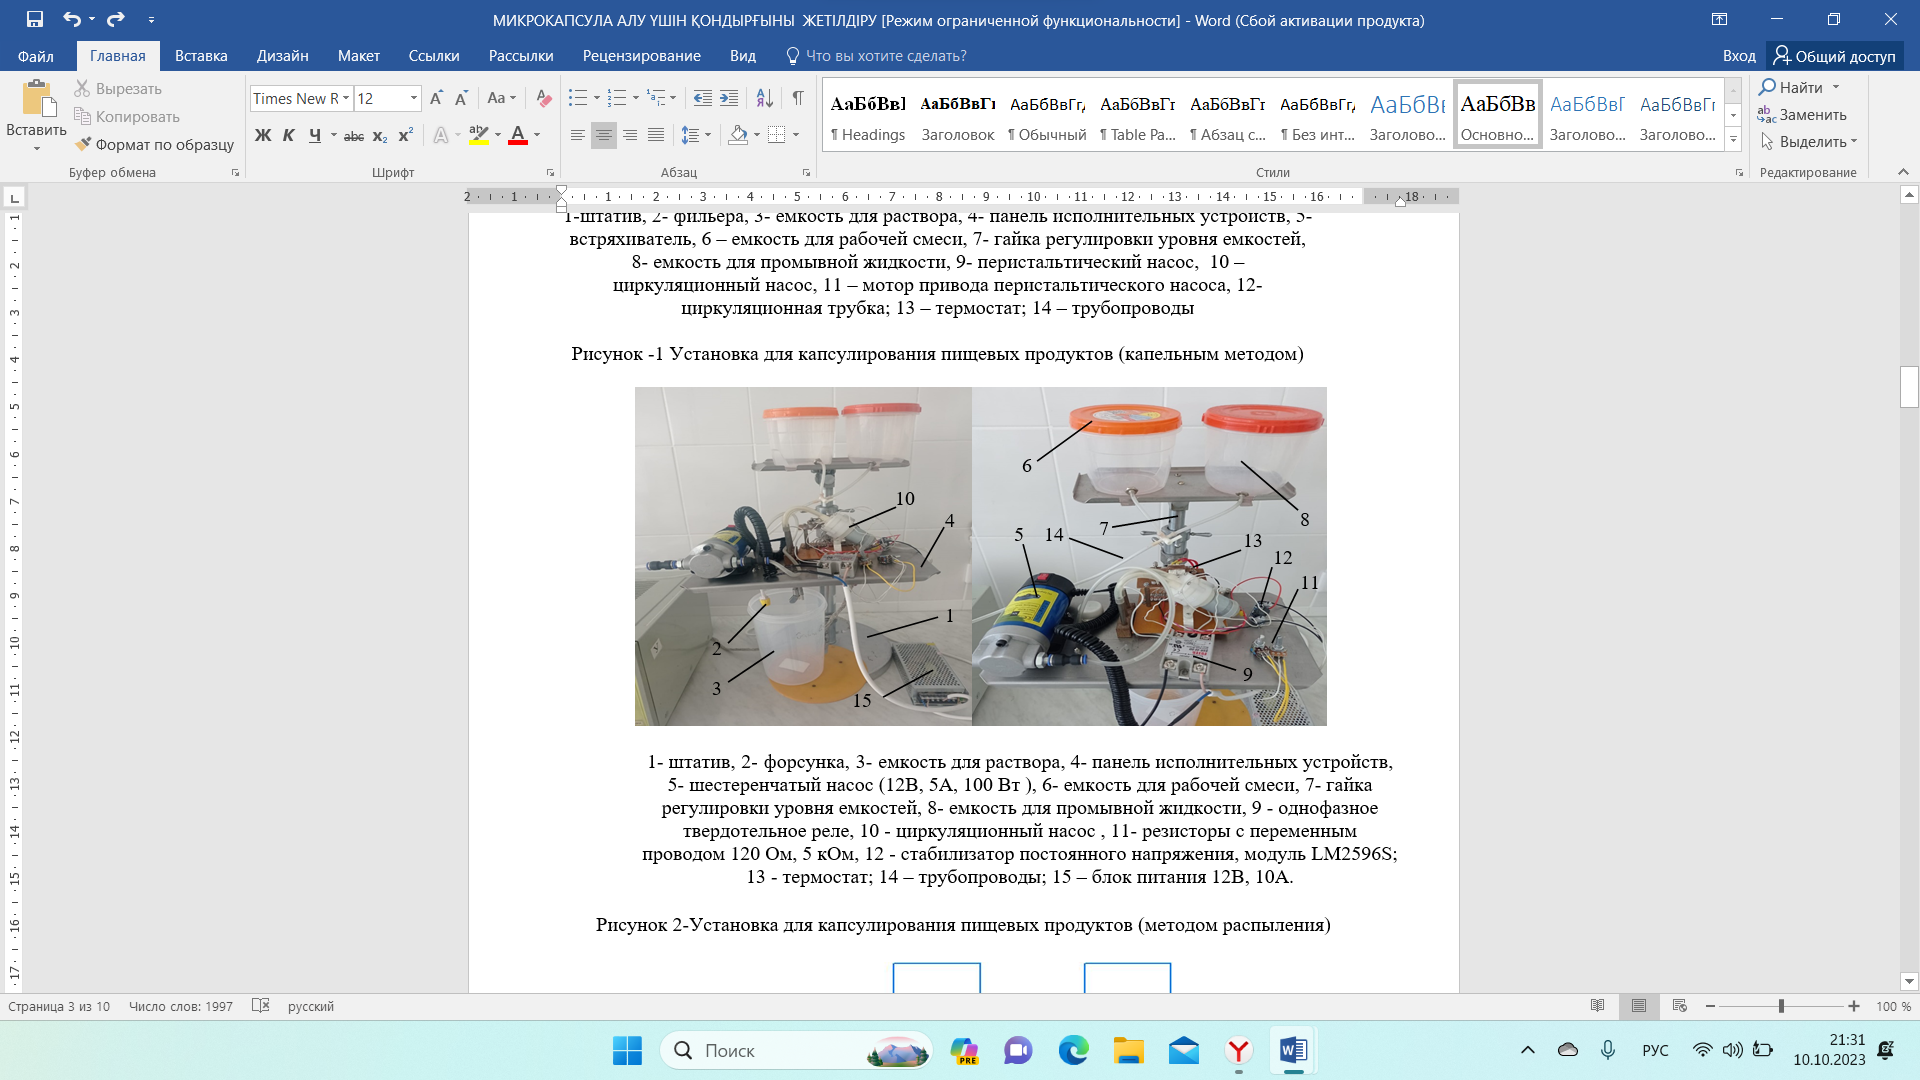
\includegraphics[width=0.8\textwidth]{assets/310}
	\caption*{}
\end{figure}

\emph{1- штатив, 2- форсунка, 3- емкость для раствора, 4- панель
исполнительных устройств, 5- шестеренчатый насос (12 В, 5 А, 100 Вт ), 6
- емкость для рабочей смеси, 7- гайка регулировки уровня емкостей, 8-
емкость для промывной жидкости, 9 - однофазное твердотельное реле, 10 -
циркуляционный насос , 11- переменные резисторы для грубой и тонкой
регулировки частоты вращения шестеренчатого насоса , 12 - стабилизатор
постоянного напряжения, модуль LM2596S; 13 - термостат; 14 --
трубопроводы; 15 -- блок питания 24 В, 20 А}.

{\bfseries Рис. 1 - Установка для капсулирования пробиотиков (методом
распыления)}

Была выбрана форсунка с выходным отверстием d=
1,2×10\textsuperscript{-3}м, как наиболее оптимальная и по
производительности, и по качесту получаемых капсул. Для подбора
оптимального процентного соотношения альгината натрия 0,5\%, 0,8\%, 1\%.
Эксперименты проводились при температурах гелеобразующей смеси от 20 до
50 ℃.

В качестве водного раствора гелеобразующей смеси использовали раствор с
добавлением альгината натрия. Раствор получили следующим образом: в воде
(60 \textsuperscript{о}С) растворили альгинат натрия в количестве 1 \%
от общего количества взятой воды. Мерный стакан с водным раствором
альгинат натрия помещается на электромагнитную мешалку с подогревом и
раствор перемешивается до полного растворения альгинат натрия.
Температура подогрева выставляется 60 \textsuperscript{о}С, так как при
температуре ниже 60 \textsuperscript{о}С альгинат натрия плохо
растворяется, а при температуре выше 60 \textsuperscript{о}С альгинат
натрия начинает комковаться. После растворения альгината натрия смесь
охладили до температуры 40°С {[}10, с.2{]}.

В полученную смесь внесли навеску штамма пропионовокислых бактерий
Propionibacterium freudenreichii. В качестве формообразующей смеси
готовится 2\% раствор хлорида кальция. Для этого берется 98 мл
дистиллированной воды и добавляется 2 грамма хлорида кальция. После
растворения хлорида кальция формообразующая смесь готова.

Технологическую схему установки, показана на рисунке 2 {[}11, с.1{]}. В
емкость 1 для рабочей смеси заливается водный раствор гелеобразующей
смеси (1\% альгината натрия). В емкость 2 заливается промывочная
жидкость для промывки системы после выполнения работы.

\begin{figure}[H]
	\centering
	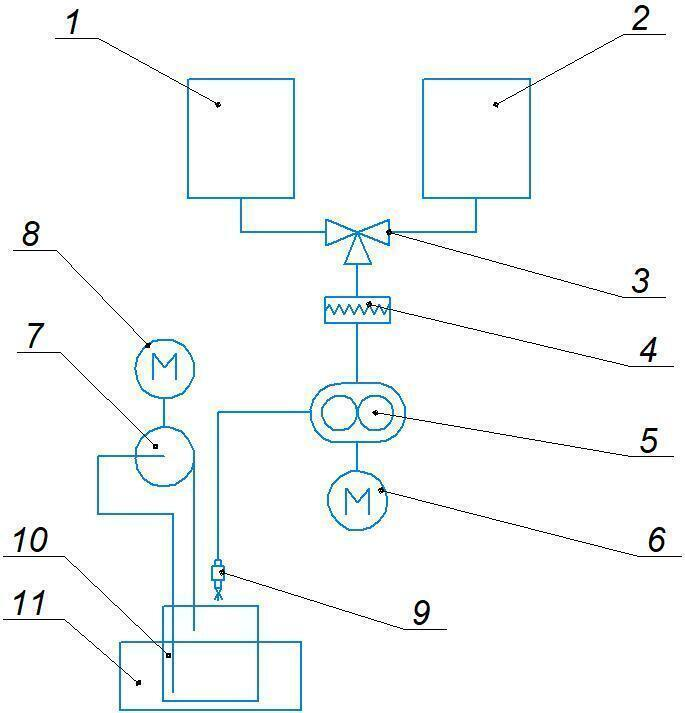
\includegraphics[width=0.8\textwidth]{assets/311}
	\caption*{}
\end{figure}

\emph{1 -- емкость для рабочей смеси; 2 -- емкость для промывной
жидкости; 3 -- вентиль-переключатель; 4 -- термостат; 5 --}
\emph{шестеренчатый насос; 6 -- мотор привода шестеренчатого насоса; 7
--} \emph{циркуляционный насос; 8 -- мотор привода циркуляционного
насоса; 9 -- форсунка; 10 -- емкость для формообразующего раствора; 11
-- емкость для охлаждения (льда)}

{\bfseries Рис. 2 - Технологическая схема установки для капсулирования}

С помощью вентиля - переключателя 3 раствор из емкостей 1 подается в
общую систему. Термостат 4 предназначен для поддержания температуры
жидкости в системе на должном уровне. (40 град).

Шестеренчатый насос 5 подает жидкость в форсунку 9, где происходит
распыление. Микрокапсулы образуются в формообразующей жидкости,
представляющий из себя хлорид кальция, за счет химического
преобразования альгината натрия в альгинат кальция при реагировании
альгината натрия с формообразующей жидкостью. Для охлаждения
формообразующей жидкости емкость 10 помещается в емкость со льдом 11.
После получения микрокапсул проводится отделение капсул от
формообразующей жидкости с помощью фильтрующей сетки (на схеме не
указано, т.к. не входит в состав оборудования) {[}10, с.3; 11, с.3{]}.

Определение вязкости водного раствора гелеобразующей смеси. Как
известно, аналоговые вискозиметры с круговой шкалой являются простыми и
удобными в использовании.

Для проведения измерений вязкости, необходимо зафиксировать основное
рабочее тело вискозиметра на вертикальной цилиндрической штанге. В
корпусе вискозиметра, на выходной вал электродвигателя крепится ротор.
Частота вращения регулятора скорости вращения ротора находится в
пределах от 0 до 100 об/мин.

Методология измерения вязкости состоит из нескольких этапов:

Подготовка пробы, путем размещения ее в химической посуде объемом не
менее 600 мл. Выбор подходящего наконечника ротора и его крепление к
выходному валу ротора. Тип необходимого наконечника определяется а
зависимости от вязкости исследуемой жидкости. С целью проведения
измерений в гелеобразных средах, необходимо использовать наконечник
ротора № 4. Использование других типов наконечников, не соответствующих
типу измеряемой смеси, не даст адекватных результатов измерения. 1.
Помещение рабочего элемента в исследуемую пробу. 2. Включение
вискозиметра. 3. Определение необходимой скорости вращения ротора. 4.
Стабилизация показаний (время стабилизации определяется в среднем после
5 оборотов ротора и находится в прямой зависимости от скорости вращения
и характеристик исследуемой жидкости). 5. Снятие показаний с круговой
шкалы.

В соответствии с номером использованного ротора и скоростью вращения,
определяется табличный коэффициент, на который нужно умножить показания
с круговой шкалы вискозиметра. Если необходимо получить данные в мПа-с,
данные с круговой шкалы вискозиметра необходимо умножить на фактор F
(табличный коэффициент), соответствующий определенному ротору {[}10,
с.4{]}.

{\bfseries Результаты и обсуждения.} Для выявления изменения значений
экспериментальных данных, построены графики зависимости вязкости
гелеобразующей смеси от температуры раствора и частоты вращения ротора
вискозиметра. Показано на рисунке 3,4,5,6. Диапазон исследуемых
температур был выбран от 20 до 50 ºС, так как при температурах ниже 20
ºС водный раствор гелеобразующей смеси загустевает и соответственно
перестает течь через форсунку, а при температурах выше 50 ºС пробиотики
погибают.

При определении вязкости в вискозиметре Брукфильда постоянный режим
выходит после частоты вращения ротора от 0,333 с\textsuperscript{-1} до
0,833 с\textsuperscript{-1}.

\begin{figure}[H]
	\centering
	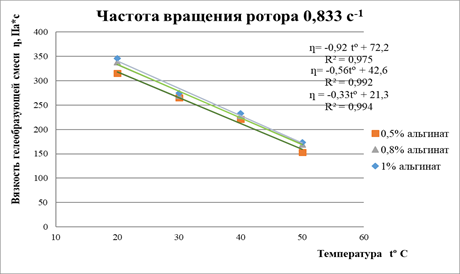
\includegraphics[width=0.8\textwidth]{assets/312}
	\caption*{}
\end{figure}

{\bfseries Рис.3 -Зависимость вязкости гелеобразующей смеси от температуры
раствора и количества}

{\bfseries альгината натрия частоты вращения ротора 0,833
с\textsuperscript{- 1}}

\begin{figure}[H]
	\centering
	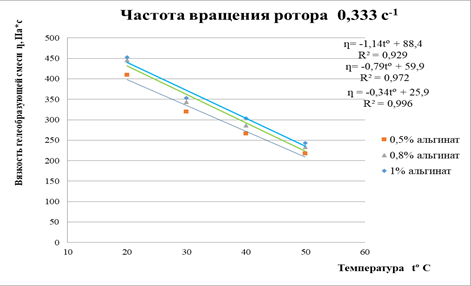
\includegraphics[width=0.8\textwidth]{assets/313}
	\caption*{}
\end{figure}

{\bfseries Рис. 4 - Зависимость вязкости гелеобразующей смеси от
температуры раствора и}

{\bfseries количества альгината натрия частоты вращения ротора 0,333
с\textsuperscript{- 1}}

Показано на рисунке 3 - 4 с раствором альгината натрия, на графике
зависимости вязкости гелеобразующей смеси от температуры раствора при
частоте вращения ротора вискозиметра 0,833 с\textsuperscript{- 1} и
0,333 с\textsuperscript{- 1} в экспериментальной установке для получения
капсул, вязкость значительно увеличивается при понижении температуры, а
по мере увеличения концентрации вязкость гелеобразующей смеси
увеличивается.

\begin{figure}[H]
	\centering
	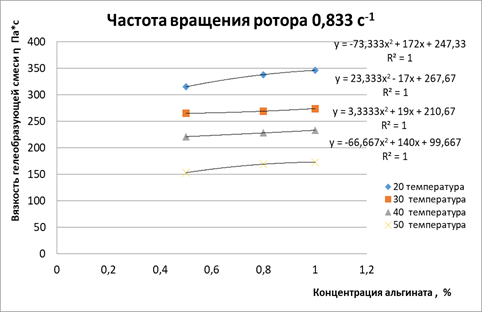
\includegraphics[width=0.8\textwidth]{assets/314}
	\caption*{}
\end{figure}

{\bfseries Рис. 5 - Зависимость вязкости гелеобразующей смеси от
концентрации раствора альгината}

{\bfseries натрия при различных температурах}

\begin{figure}[H]
	\centering
	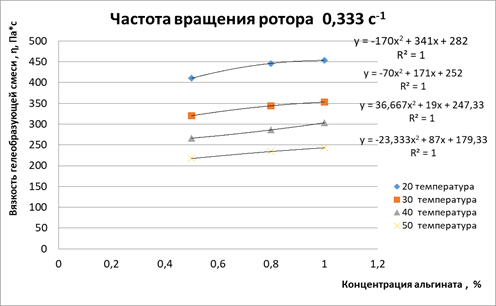
\includegraphics[width=0.8\textwidth]{assets/315}
	\caption*{}
\end{figure}

{\bfseries Рис. 6 - Зависимость вязкости гелеобразующей смеси от
концентрации}

{\bfseries раствора альгината натрия при различных температурах}

Зависимость вязкости гелеобразующей смеси от концентрации раствора
альгината натрия при различных температурах, из графиков на рисунке 5 -
6 видно, что при температурах 40 и 50 С° величина вязкости незначительно
изменяется для частоты вращения ротора, но для предотвращения гибели
пробиотических микроорганизмов не рекомендуется использовать температуру
выше 50 С°\emph{{\bfseries .}} Исходя из всего этого, наиболее подходящая
температура для использования раствора составляет 40 С°.

В условиях напряженного состояния, при приложении силы, поведение
неньютоновских жидкостей характеризуется напряжением, геометрическими
размерами канала и скоростью истечения жидкости {[}12{]}.

Модели, которые характеризуются упругостью и вязкостью, составляют
совокупность тел механической модели реологического тела продукта. Их
деформационное поведение описывается реологическими уравнениями {[}12,
с.14{]}.

Гелеобразное сырье при нагнетании давления с помощью шестеренчатого
насоса испытывает мгновенно-упругую деформацию (G) и в дальнейшем, при
напряжении превышающем предел текучести (θт), вязкопластическую (η)
деформацию. Под действием давления и испытываемых деформаций,
гелеобразное сырье попадает в форсунку, разбрызгивается, в дальнейшем
образует микрокапсулы.

Используя механические модели Бингама {[}12, с.18{]}, Шведова {[}13{]},
Шоффильда-Скоттблера {[}14{]}, Пелега {[}15{]} и проведения обоснования
с целью описания поведения гелеобразного сырья при механическом
воздействии, можно получить механическую модель реологического тела.
Данная модель реологического тела представляет собой модель Бюргерса
{[}16{]} в соответствии с рисунком 7 {[}10, с.9; 12, с.20{]}, т.е.
последовательную механическую модель вязко - упругого релаксирующего
тела Максвелла и вязко - упругого тела Кельвина -- Фойгта для
гелеобразной среды.

Таким образом, общая деформация гелеобразного сырья для данной модели
представляет собой сумму деформаций тела Максвелла и элемента,
моделирующего поведение сырья, которое отражает явление упругого
последствия, представляющее собой изменение упругой деформации с
течением времени

% \begin{longtable}[]{@{}
%   >{\raggedright\arraybackslash}p{(\columnwidth - 4\tabcolsep) * \real{0.4726}}
%   >{\raggedright\arraybackslash}p{(\columnwidth - 4\tabcolsep) * \real{0.3823}}
%   >{\raggedright\arraybackslash}p{(\columnwidth - 4\tabcolsep) * \real{0.1451}}@{}}
% \toprule\noalign{}
% \begin{minipage}[b]{\linewidth}\raggedright
% \begin{figure}[H]
% 	\centering
% 	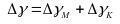
\includegraphics[width=0.8\textwidth]{assets/316}
% 	\caption*{}
% \end{figure},
% \end{minipage} & \begin{minipage}[b]{\linewidth}\raggedright
% \end{minipage} & \begin{minipage}[b]{\linewidth}\raggedright
% (1)
% \end{minipage} \\
% \midrule\noalign{}
% \endhead
% \bottomrule\noalign{}
% \endlastfoot
% \end{longtable}

где, \emph{∆γ\textsubscript{М}}-- деформация модели Максвелла;

\emph{∆γ\textsubscript{К}} - деформация модели Кельвина -- Фойгта

\begin{figure}[H]
	\centering
	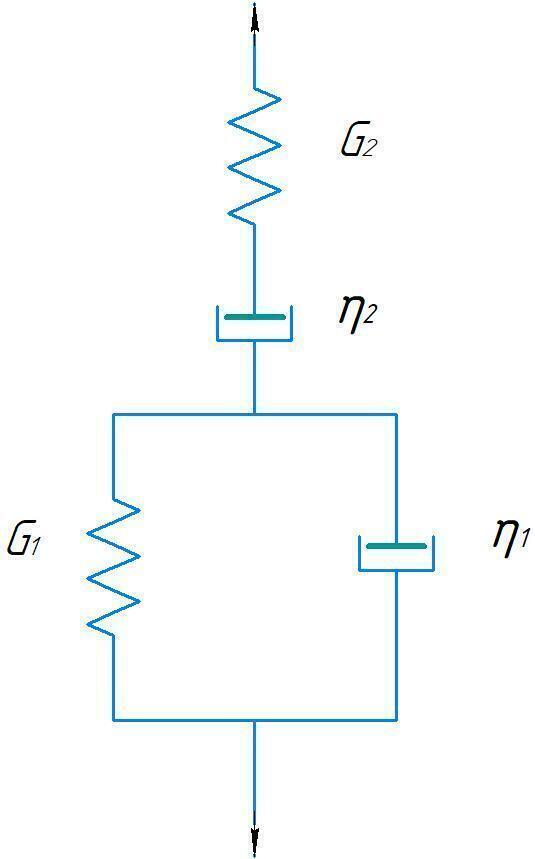
\includegraphics[width=0.8\textwidth]{assets/317}
	\caption*{}
\end{figure}

\emph{G\textsubscript{1} - модуль мгновенной эластичной деформации, Па;
G\textsubscript{2} - модуль замедленной упругой деформации, Па;
η\textsubscript{1} -- ньютоновская вязкость, Па·с; η\textsubscript{2}
--пластическая вязкость при сдвиге, Па·с}

{\bfseries Рис. 7 -- Механическая модель Бюргерса}

Производная по времени от левой и правой частей уравнения (1) имеет вид:

% \begin{longtable}[]{@{}
%   >{\raggedright\arraybackslash}p{(\columnwidth - 2\tabcolsep) * \real{0.8059}}
%   >{\raggedright\arraybackslash}p{(\columnwidth - 2\tabcolsep) * \real{0.1941}}@{}}
% \toprule\noalign{}
% \begin{minipage}[b]{\linewidth}\raggedright
% \begin{figure}[H]
% 	\centering
% 	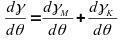
\includegraphics[width=0.8\textwidth]{assets/318}
% 	\caption*{}
% \end{figure}.
% \end{minipage} & \begin{minipage}[b]{\linewidth}\raggedright
% (2)
% \end{minipage} \\
% \midrule\noalign{}
% \endhead
% \bottomrule\noalign{}
% \endlastfoot
% \end{longtable}

Реологическое уравнение модели Максвелла {[}12, с.17{]} определяет
величину \begin{figure}[H]
	\centering
	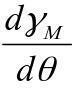
\includegraphics[width=0.8\textwidth]{assets/319}
	\caption*{}
\end{figure}:

% \begin{longtable}[]{@{}
%   >{\raggedright\arraybackslash}p{(\columnwidth - 2\tabcolsep) * \real{0.7850}}
%   >{\raggedright\arraybackslash}p{(\columnwidth - 2\tabcolsep) * \real{0.2150}}@{}}
% \toprule\noalign{}
% \begin{minipage}[b]{\linewidth}\raggedright
% \begin{figure}[H]
% 	\centering
% 	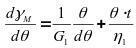
\includegraphics[width=0.8\textwidth]{assets/320}
% 	\caption*{}
% \end{figure}
% \end{minipage} & \begin{minipage}[b]{\linewidth}\raggedright
% (3)
% \end{minipage} \\
% \midrule\noalign{}
% \endhead
% \bottomrule\noalign{}
% \endlastfoot
% \end{longtable}

Величина \begin{figure}[H]
	\centering
	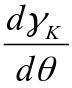
\includegraphics[width=0.8\textwidth]{assets/321}
	\caption*{}
\end{figure} определяется реологическим
уравнением модели Кельвина - Фойгта {[}17, 12, с.16{]}:

\begin{longtable}[]{@{}
  >{\raggedright\arraybackslash}p{(\columnwidth - 2\tabcolsep) * \real{0.8472}}
  >{\raggedright\arraybackslash}p{(\columnwidth - 2\tabcolsep) * \real{0.1528}}@{}}
\toprule\noalign{}
\begin{minipage}[b]{\linewidth}\raggedright
\[\frac{d\gamma_{K}}{d\theta} = \left( \frac{\theta}{G_{2} \cdot d\theta} \right) \cdot \lbrack 1 - e^{( - G_{2} \cdot t/\eta_{2})}\rbrack\]
\end{minipage} & \begin{minipage}[b]{\linewidth}\raggedright
(4)
\end{minipage} \\
\midrule\noalign{}
\endhead
\bottomrule\noalign{}
\endlastfoot
\end{longtable}

Подставляя это значение в выражение (2) получим уравнение Бюргерса для
гелеобразного сырья {[}12, с.19{]}:

\begin{longtable}[]{@{}
  >{\raggedright\arraybackslash}p{(\columnwidth - 2\tabcolsep) * \real{0.8422}}
  >{\raggedright\arraybackslash}p{(\columnwidth - 2\tabcolsep) * \real{0.1578}}@{}}
\toprule\noalign{}
\begin{minipage}[b]{\linewidth}\raggedright
\[\dot{\gamma} = \frac{\theta}{G_{1}} + \frac{\theta \cdot t}{\eta_{1}} + (\frac{\theta}{G_{2}}) \cdot \lbrack 1 - e^{( - G_{2} \cdot t/\eta_{2})}\rbrack\]
\end{minipage} & \begin{minipage}[b]{\linewidth}\raggedright
(5)
\end{minipage} \\
\midrule\noalign{}
\endhead
\bottomrule\noalign{}
\endlastfoot
\end{longtable}

где: \begin{figure}[H]
	\centering
	
\includegraphics[width=0.8\textwidth]{assets/322}
	\caption*{}
\end{figure} - градиент скорости,
с\textsuperscript{-1}; \emph{G\textsubscript{1}} - модуль мгновенной
эластичной деформации, Па; \emph{G\textsubscript{2}} - модуль
замедленной упругой деформации, Па; \emph{η\textsubscript{1}} --
ньютоновская вязкость, Па·с; \emph{η\textsubscript{2}} --пластическая
вязкость при сдвиге, Па·с; \emph{θ} -- касательное напряжение, Па;
\emph{t} -- время, с.

Полученная математическая модель с достаточной точностью позволит
описать процесс истечения гелеобразной жидкости из форсунки для
экспериментальной установки. Представленная модель применима к
установкам с подобным принципом действия, вне зависимости от их
габаритов {[}10, с.10{]}.

Для получения микрокапсул эксперимент проводили с применением форсунки с
выходным отверстием d= 1,2×10\textsuperscript{-3}м {[}10, с.6-7{]}.

\begin{figure}[H]
	\centering
	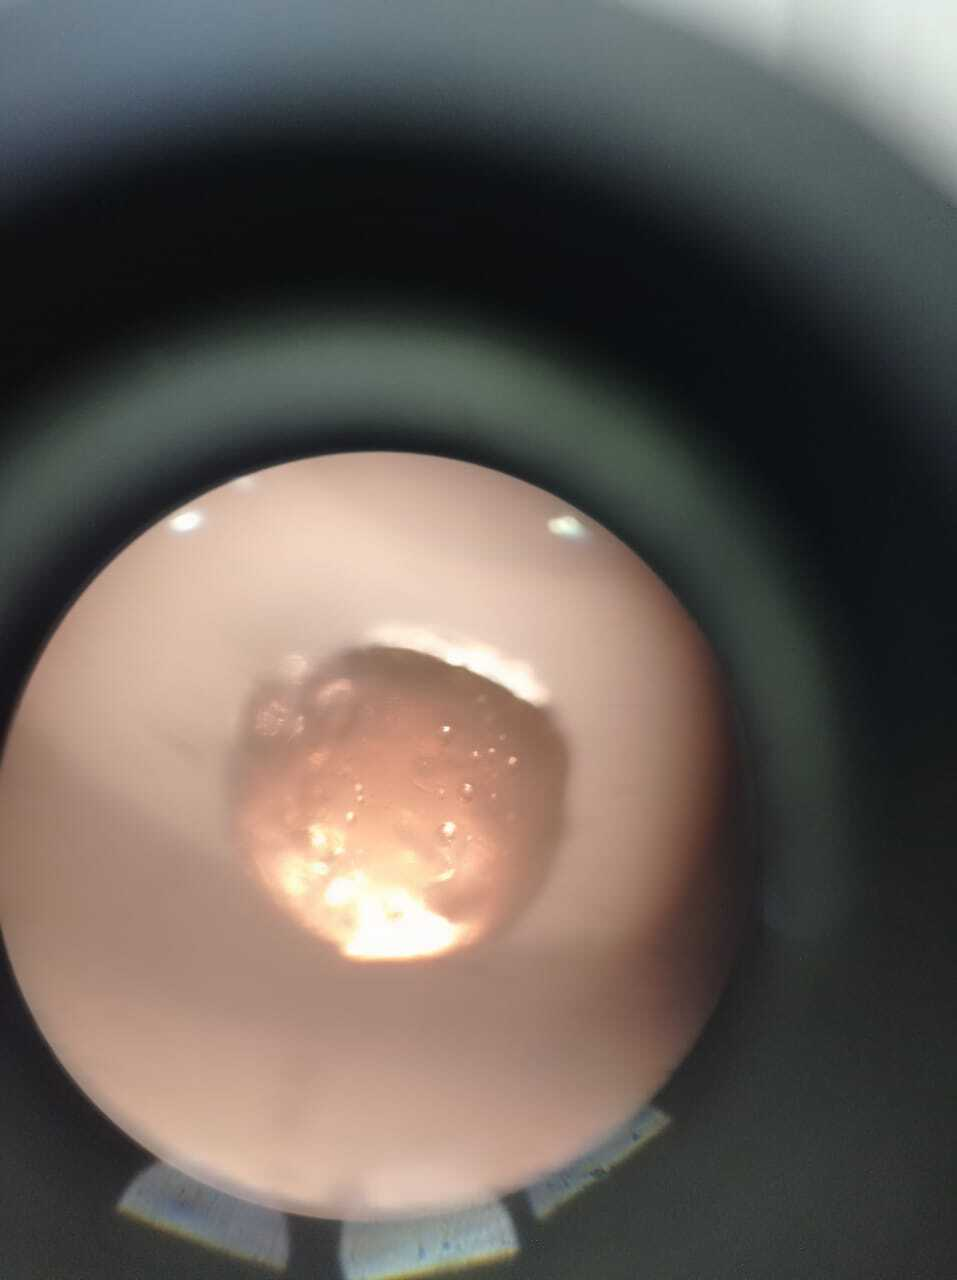
\includegraphics[width=0.8\textwidth]{assets/323}
	\caption*{}
\end{figure}

{\bfseries Рис. 8- Микрокапсула 0,5\% альгинат натрия}

При концентрации 0,5\% альгината натрия полученные капсулы имеют
округлую, но не всегда правильную форму и однородную структуру, мягкую
консистенцию, легко разрушаются при физическом воздействии и имеют
средний размер 1,2 · 10 \textsuperscript{-3}м.

\begin{figure}[H]
	\centering
	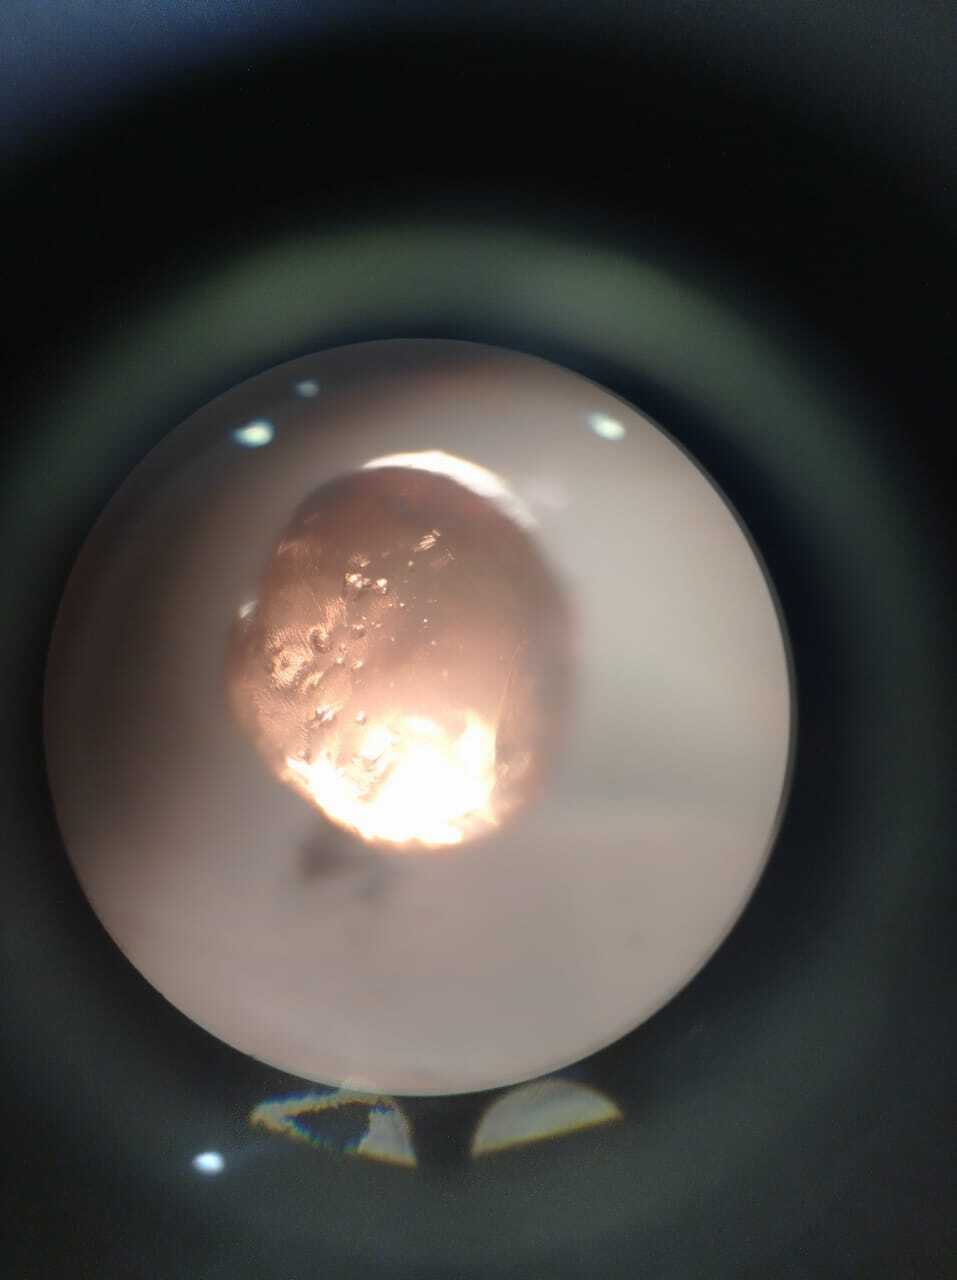
\includegraphics[width=0.8\textwidth]{assets/324}
	\caption*{}
\end{figure}

{\bfseries Рис. 9 -Микрокапсула 0,8\% альгинат натрия}

При концентрации 0,8\% альгината натрия полученные капсулы имеют
округлую форму и однородную структуру, мягкую консистенцию, легко
разрушаются при физическом воздействии и имеют средний размер
1,3×10\textsuperscript{-3}м.

\begin{figure}[H]
	\centering
	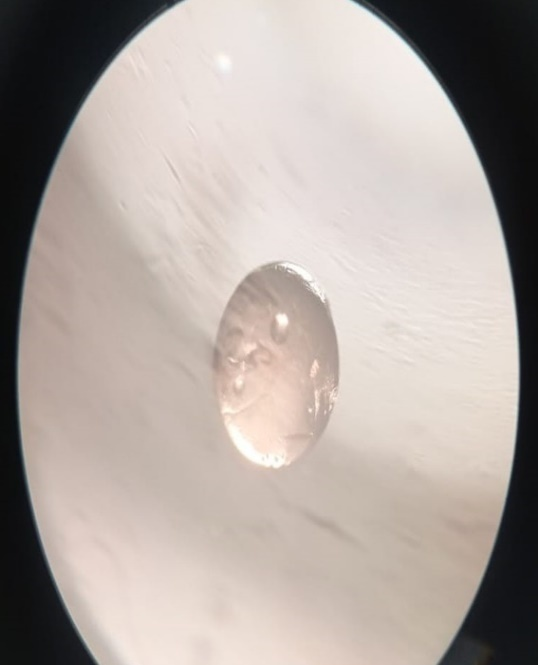
\includegraphics[width=0.8\textwidth]{assets/325}
	\caption*{}
\end{figure}

{\bfseries Рис.10- Микрокапсула 1 \% альгинат натрия}

При концентрации 1\% альгината натрия полученные капсулы имеют округлую
форму и однородную структуру, мягкие на ощупь, но устойчивые при
физическом воздействии и имеют средний размер составил
1,4×10\textsuperscript{-3}м

Проводя анализ капсул, можно сделать вывод: что наиболее оптимальным
вариантом является состав раствора, содержащий 1\% альгинат натрия.
Капсулы, изготовленные из этого раствора, имеют красивую округлую форму,
одинаковый размер, мягкую консистенцию, но устойчивую для физического
воздействия.

{\bfseries Выводы.} В настоящее время микрокапсулы стали применяться в
сельском хозяйстве, фармацевтике в различных отраслях промышленности.
При проведении экспериментов использовали в качестве распылителя
пластиковую форсунку с выходным диаметром d=
1,2×10\textsuperscript{-3}м. Для экспериментов готовили растворы в
концентрациях 0,5\%, 0,8\%, 1\% альгината. Для подбора оптимальных
размеров капсул построены графики зависимости вязкости гелеобразующей
смеси от температуры раствора и скорости вращения вискозиметра ротора.
Исследуемый диапазон температур выбирался от 20 до 50 ºС. Для
определения изменения значений экспериментальных данных построены
графики зависимости вязкости гелеобразующей смеси от температуры
раствора и концентрации раствора при различных температурах.

В конечном итоге, получили округлые капсулы, содержащие пробиотик
Propionibacterium freudenreichii, которые могут быть использованы в
дальнейших технологических процессах при получении пищевых продуктов
лечебно-профилактического действия или при получении фармокологических
препаратов.

{\bfseries Литература}

1. Жумадилова Г. А. Исследование процесса инкапсулирования пробиотиков с
целью создания оборудования: дисс \ldots{} PhD - 6D072400. - Семей: НАО
«Университет имени Шакарима города Семей», 2020.- 131с.

2. Какимов А.К., Ибрагимов Н.К., Муратбаев А.М., Джумажанова М.М.,
Жумадилова Г.А. Инкапсулирование в пищевой промышлености // Пищевые
инновации и биотехнологии: сборник тезисов VII Международной научной
конференции студентов, аспирантов и молодых ученых. Т. 1. Технологии
пищевых производств, качество и безопасность / под общ. ред. А. Ю.
Просекова: ФГБОУ ВО «Кемеровский государственный университет».-Кемерово,
2019. - С. 153-154.

3. A.Kakimov, Kakimova Zh., Mirasheva G., Bepeyeva A., Toleubekova S.,
Jumazhanova M., Zhumadilova G., Yessimbekov Zh. Amino Acid Composition
of Sour-milk Drink with Encapsulated Probiotics // Annual Research \&
Review in Biology.- 2017.- Vol.18(1).- P.1-7.

DOI 10.9734/ARRB/2017/36079

4. Какимов А.К., Какимова Ж.Х., Бепеева А.Е., Джумажанова М.М,
Жумадилова Г.А. Безопасность, функциональные и технологические свойства
пробиотических бактерий // Сборник научных трудов, посвященный 60-летию
отдела сибниис федеральное государственное бюджетное научное учреждение
Фанца. Актуальные проблемы техники и технологии переработки молока,
Барнаул: 2018.- C.-162-165

5. Муратбаев А. М. Капсулаланған биологиялық белсенді қоспаларды
қолданып өндірілген,тамақ өнімдерінің қауіпсіздігін қамтамасыз етудің
тәжірибелік аспектілері: дисс. ...РhD - 6D073500. -- Семей: Семей
қаласының Шәкәрім атындағы университеті, 2021. -- 169 с.

6. Burgain J., Gaiani C., Linder M., Scher J. Encapsulation of probiotic
living cells: From laboratory scale to industrial applications// Journal
of Food Engineering.-2011.-Vol.104(4) - Р.467--483. DOI
10.1016/j.jfoodeng.2010.12.031

7. Rowley J.A., Madlambayan G., Mooney D.J. Alginate hydrogels as
synthetic extracellular matrix materials//Biomaterials.- 1999.-Vol. 20
(1).- Р. 45- 53.

DOI~10.1016/s0142-9612(98)00107-0

8. Krasaekoopt W., Bhandari B., Deeth H. Evaluation of encapsulation
techniques of probiotics for yoghurt //International Dairy
Journal.-2003.- Vol.13(1).- Р. 3--13.

DOI 10.1016/S0958-6946(02)00155-3

9. Cook M.T., Tzortzis G., Charalampopoulos D.,. Khutoryanskiy V. V.
Microencapsulation of probiotics for gastrointestinal delivery. Review//
Journal of Controlled Release. - 2012.- Vol.162 - Р. 56 - 67. DOI
10.1016/j.jconrel.2012.06.003

10. M. Tashybayeva, A. Kakimov, N. Ibragimov, G. Zhumadilova, А.
Muratbayev, M. Jumazhanova, B. Idyryshev, Z. Kapshakbayeva, A. Bepeyeva
Optimization of encapsulation parameters for sodium alginate capsules: A
study on the effect of temperature and gear pump rotation speed on
capsule production and quality// Journal of Food Process Engineering.-
2024- Vol.47(7) DOI 10.1111/jfpe.14687

11. Ташыбаева М.М., Какимов А.К., Майоров А.А., Ибрагимов Н.К.,
Джумажанова М.М., Жумадилова Г.А., Муратбаев А.М., Бакиева А.Б.,
Дукенбаев Д.К. Капсулаған өнімдерді өндіруге арналған қондырғы / ҚР
пайдалы модельге патенті № 9093, 03.05.2024ж.

12. Мачихин Ю.А., Мачихин С.А. Инженерная реология пищевых продуктов. -
М.: Легкая и пищевая промышленность.- 1981.-215 с.

13. Sсhоfie1d R. K., Scott Blair G. W. The relationschip between
viscosity, elasticity and plastics strenght of a soft material as
illustrated by some mechanical properties of flour dough. --- Proc. Roy.
Soc.-1932. - P. 707- 718.DOI 10.1098/pspa.1933.0038

14. Scott Blair G. W. Psycho-rheology. --- J. Texture Studies, 1.-
1970.- P. 231

15. Реleg M. Contact and fracture elements as components of the
rheolo-gical memory of solid foods. --- J. Texture Studies 8, 1977. - P.
39 - 48. DOI~10.1111/j.1745-4603.1977.tb01164.x

16. Шрам Г. Основы практической реологии и реометрии -- М.: Колос С,
2003. -- 312 с.

ISBN 5-9532-0234-2

17.Горбатов А.В., Реология мясных и молочных продуктов. -- М.: Пищевая
промышленность, 1979. -- 383 с.

{\bfseries References}

1. Zhumadilova G. A. Issledovanie processa inkapsulirovanija probiotikov
s cel\textquotesingle ju sozdanija oborudovanija: diss \ldots{} PhD -
6D072400. - Semej: NAO «Universitet imeni Shakarima goroda Semej»,
2020.- 131s. {[}in Russian{]}

2. Kakimov A.K., Ibragimov N.K., Muratbaev A.M., Dzhumazhanova M.M.,
Zhumadilova G.A. Inkapsulirovanie v pishhevoj promyshlenosti //
Pishhevye innovacii i biotehnologii: sbornik tezisov VII Mezhdunarodnoj
nauchnoj konferencii studentov, aspirantov i molodyh uchenyh. T. 1
Tehnologii pishhevyh proizvodstv, kachestvo i
bezopasnost\textquotesingle{} / pod obshh. red. A. Ju. Prosekova: FGBOU
VO «Kemerovskij gosudarstvennyj universitet».-Kemerovo, 2019. - S.
153-154{\bfseries .} {[}in Russian{]}

3. A.Kakimov, Kakimova Zh., Mirasheva G., Bepeyeva A., Toleubekova S.,
Jumazhanova M., Zhumadilova G., Yessimbekov Zh. Amino Acid Composition
of Sour-milk Drink with Encapsulated Probiotics // Annual Research \&
Review in Biology.- 2017.- Vol.18(1).- P.1-7.

DOI 10.9734/ARRB/2017/36079

4. Kakimov A.K., Kakimova Zh.H., Bepeeva A.E., Dzhumazhanova M.M,
Zhumadilova G.A. Bezopasnost\textquotesingle,
funkcional\textquotesingle nye i tehnologicheskie svojstva
probioticheskih bakterij // Sbornik nauchnyh trudov, posvjashhennyj
60-letiju otdela sibniis federal\textquotesingle noe gosudarstvennoe
bjudzhetnoe nauchnoe uchrezhdenie Fanca. Aktual\textquotesingle nye
problemy tehniki i tehnologii pererabotki moloka, Barnaul: 2018.-
C.-162-165. {[}un Kazakh{]}

5. Muratbaev A. M. Kapsulalanғan biologijalyқ belsendі қospalardy
қoldanyp өndіrіlgen,tamaқ өnіmderіnің қauіpsіzdіgіn қamtamasyz etudің
tәzhіribelіk aspektіlerі: diss. ...RhD - 6D073500. -Semej: Semej
қalasynyң Shәkәrіm atyndaғy universitetі, 2021. -169 s.

6. Burgain J., Gaiani C., Linder M., Scher J. Encapsulation of probiotic
living cells: From laboratory scale to industrial applications// Journal
of Food Engineering.-2011.-Vol.104(4) - Р.467--483. DOI
10.1016/j.jfoodeng.2010.12.031

7. Rowley J.A., Madlambayan G., Mooney D.J. Alginate hydrogels as
synthetic extracellular matrix materials//Biomaterials.- 1999.-Vol. 20
(1).- Р. 45- 53.

DOI~10.1016/s0142-9612(98)00107-0

8. Krasaekoopt W., Bhandari B., Deeth H. Evaluation of encapsulation
techniques of probiotics for yoghurt //International Dairy
Journal.-2003.- Vol.13(1).- Р. 3--13.

DOI 10.1016/S0958-6946(02)00155-3

9. Cook M.T., Tzortzis G., Charalampopoulos D.,. Khutoryanskiy V. V.
Microencapsulation of probiotics for gastrointestinal delivery. Review//
Journal of Controlled Release. - 2012.- Vol.162 - Р. 56 - 67. DOI
10.1016/j.jconrel.2012.06.003

10. M. Tashybayeva, A. Kakimov, N. Ibragimov, G. Zhumadilova, А.
Muratbayev, M. Jumazhanova, B. Idyryshev, Z. Kapshakbayeva, A. Bepeyeva
Optimization of encapsulation parameters for sodium alginate capsules: A
study on the effect of temperature and gear pump rotation speed on
capsule production and quality// Journal of Food Process Engineering.-
2024- Vol.47(7) DOI 10.1111/jfpe.14687

11. Tashybaeva M.M., Kakimov A.K., Majorov A.A., Ibragimov N.K.,
Dzhumazhanova M.M., Zhumadilova G.A., Muratbaev A.M., Bakieva A.B.,
Dukenbaev D.K. Kapsulaғan өnіmderdі өndіruge arnalғan қondyrғy / ҚR
pajdaly model\textquotesingle ge patentі № 9093, 03.05.2024zh. {[}in
Russian{]}

12. Machihin Ju.A., Machihin S.A. Inzhenernaja reologija pishhevyh
produktov. - M.: Legkaja i pishhevaja promyshlennost\textquotesingle.-
1981.-215 s. {[}in Russian{]}

13. Sсhоfie1d R. K., Scott Blair G. W. The relationschip between
viscosity, elasticity and plastics strenght of a soft material as
illustrated by some mechanical properties of flour dough. --- Proc. Roy.
Soc.-1932. - P. 707- 718.DOI 10.1098/pspa.1933.0038 {[}in Russian{]}

14. Scott Blair G. W. Psycho-rheology. --- J. Texture Studies, 1.-
1970.- P. 231. {[}in Russian{]}

15. Реleg M. Contact and fracture elements as components of the
rheolo-gical memory of solid foods. --- J. Texture Studies 8, 1977. - P.
39 - 48. DOI~10.1111/j.1745-4603.1977.tb01164.x

16. Shram G. Osnovy prakticheskoj reologii i reometrii -- M.: Kolos S,
2003. -- 312 s.

ISBN 5-9532-0234-2

17.Gorbatov A.V., Reologija mjasnyh i molochnyh produktov. -M.:
Pishhevaja promyshlennost\textquotesingle, 1979. - 383 s.

\emph{{\bfseries Сведения об авторах}}

Ташыбаева М.М.-докторант, Университет имени Шакарима города Семей,
Казахстан, е-mail: marzhan06081990@gmail.com.

Какимов А.К.- доктор технических наук, профессор, Университет имени
Шакарима города Семей, Казахстан, е-mail: bibi.53@mail.ru;

Майоров А.А. - доктор технических наук, профессор ФГБНУ Федеральный
Алтайский научный центр агробиотехнологий, Барнаул, Российская
Федерация, е-mail: maiorov.alex@mail.ru;

Жумадилова Г.А. - PhD, Университет имени Шакарима города Семей,
Казахстан; е- mail: zhumadilovaga@mail.ru.

\emph{{\bfseries Information about the authors}}

Tashybayeva M.М{\bfseries .} - doctoral student, Shakarim University of
Semey, Kazakhstan, e-mail: marzhan06081990@gmail.com;

Kakimov А.К. -- doctor of technical sciences, Shakarim University of
Semey, Kazakhstan,

e-mail: bibi.53@mail.ru;

Mayorov A.А. - doctor of technical sciences, professorederal State
Budget Scientific Institution Federal Altai Scientific Center for
Agrobiotechnologies , Barnaul, Russian, e-mail: maiorov.alex@mail.ru;

Zhumadilova G.А.{\bfseries -} PhD, Shakarim University of Semey,
Kazakhstan; e-mail: zhumadilovaga@mail.ru.\newpage
{\bfseries МРНТИ 65.59.23}, 62.13.02

{\bfseries ПРИМЕНЕНИЕ БИОТЕХНОЛОГИЧЕСКИХ МЕТОДОВ УЛУЧШЕНИЯ КАЧЕСТВА КОНИНЫ
ПРИ ПЕРЕРАБОТКЕ}

{\bfseries \textsuperscript{1}С.Л. Гаптар, \textsuperscript{2}С.Б.
Байтукенова\textsuperscript{🖂}}

\textsuperscript{1}ФГБОУ ВО «Новосибирский государственный аграрный
университет», Новосибирск, Россия,

\textsuperscript{2}АО «Казахский университет технологии и бизнеса имени
К.Кулажанова», Астана, Казахстан,

{\bfseries \textsuperscript{🖂}}Корреспондент-автор: saule7272@mail.ru

В данной работе рассматриваются современные биотехнологические методы,
направленные на улучшение качества конины. Рассматриваются принципы их
действия, влияние на структуру, вкус и питательные свойства мяса.

Для оптимизации производственного цикла и улучшения качества соленых
мясопродуктов, особенно из конины с высокой жесткостью, рекомендуется
использовать биотехнологические и физические методы обработки. Одним из
эффективных подходов является использование парного мяса, которое
обладает высокой влагосвязывающей способностью и выраженными
бактериостатическими свойствами, что замедляет рост микробов. Для
ускорения процессов посола и созревания применяют методы, такие как
электростимуляция, шприцевание и механическая обработка. Результаты
показывают, что опытные образцы соленой конины содержат больше влаги и
имеют лучшую влагосвязывающую способность, что улучшает выход и сочность
продукта. При этом прочностные характеристики у них ниже на 32\% по
сравнению с контрольными образцами. Микробиологические показатели
соответствуют нормам, хотя на начальной стадии механической обработки
наблюдается небольшой рост микроорганизмов. Тепловая обработка и
использование парного сырья способствуют качеству продукта, а применение
13\% посола и 6 часов циклической механической обработки ускоряет
процесс посола и улучшает физико-химические свойства мяса.

{\bfseries Ключевые слова:} конина, биотехнологические методы, посол мяса,
физико-химические показатели, структурно-механические свойства.

{\bfseries ӨҢДЕУ КЕЗІНДЕ ЖЫЛҚЫ ЕТІНІҢ САПАСЫН ЖАҚСАРТУДЫҢ БИОТЕХНОЛОГИЯЛЫҚ
ӘДІСТЕРІН ҚОЛДАНУ}

{\bfseries \textsuperscript{1}С.Л. Гаптар, \textsuperscript{2}С.Б.
Байтукенова\textsuperscript{🖂}}

\textsuperscript{1}Новосибирск мемлекеттік аграрлық университеті,
Новосибирск, Ресей,

\textsuperscript{2} Қ.Құлажанов атындағы Қазақ технология және бизнес
университеті, Астана, Қазақстан,

e-mail: saule7272@mail.ru

Бұл мақалада жылқы етінің сапасын жақсартуға бағытталған заманауи
биотехнологиялық әдістер қарастырылады. Олардың әрекет ету принциптері
ет құрылымына, дәмі мен тағамдық қасиеттеріне әсері қарастырылады.

Өндірістік циклды оңтайландыру және тұзды ет өнімдерінің сапасын
жақсарту үшін, әсіресе қаттылығы жоғары жылқы етінен биотехнологиялық
және физикалық өңдеу әдістерін қолдану ұсынылады. Тиімді тәсілдердің
бірі - ылғалмен байланысу қабілеті жоғары және микробтардың өсуін
бәсеңдететін айқын бактериостатикалық қасиеттері бар балғын етті
қолдану. Тұздау және жетілу процестерін жеделдету үшін
электрстимуляциялау, шприцтеу және өңдеу сияқты әдістер қолданылады.
Зерттеу нәтижелері көрсеткендей, тәжірибелік үлгіде тұздалған жылқы
етінің ылғалы көп және ылғалмен байланысу қабілеті жоғары, яғни өнімнің
өнімділігі мен шырындылығын жақсартады. Бұл жағдайда олардың беріктік
сипаттамалары бақылау үлгілерімен салыстырғанда 32\%-ға төмен.
Микробиологиялық көрсеткіштер нормаларға сәйкес келеді, дегенмен
өңдеудің бастапқы кезеңінде микроорганизмдердің аз өсуі байқалады.
Термиялық өңдеу және балғын ет шикізатын пайдалану өнімнің сапасына
ықпал етеді, ал 13\% тұзды және 6 сағаттық циклдік өңдеуді қолдану
тұздау процесін тездетеді және физика-химиялық қасиеттерін жақсартады.

{\bfseries Түйін сөздер:} жылқы еті, биотехнологиялық әдістер, етті тұздау,
физика-химиялық көрсеткіштер, құрылымдық-механикалық қасиеттер.

{\bfseries THE USE OF BIOTECHNOLOGICAL METHODS TO IMPROVE THE QUALITY}

{\bfseries OF HORSE MEAT DURING PROCESSING}

{\bfseries \textsuperscript{1}S.L. Gaptar, \textsuperscript{2}}
{\bfseries S.B. Baitukenova\textsuperscript{🖂}}

\textsuperscript{1}Novosibirsk State Agrarian University, Novosibirsk,
Russia,

\textsuperscript{2} Kazakh University of Technology and Business named
after K. Kulazhanov, Astana, Kazakhstan,

e-mail: saule7272@mail.ru

This paper considers modern biotechnological methods aimed at improving
the quality of horse meat. The principles of their action, influence on
the structure, flavor and nutritional properties of meat are considered.

To optimize the production cycle and improve the quality of salted meat
products, especially from horsemeat with high hardness, it is
recommended to use biotechnological and physical processing methods. One
of the effective approaches is the use of steam meat, which has a high
moisture-binding capacity and pronounced bacteriostatic properties,
which slows down the growth of microbes. Methods such as electrical
stimulation, syringing and mechanical treatment are used to accelerate
salting and ripening processes. The results show that experimental
samples of salted horsemeat contain more moisture and have better
moisture-binding capacity, which improves the yield and juiciness of the
product. At the same time, their strength characteristics are lower by
32\% compared to control samples. Microbiological parameters correspond
to the norms, although at the initial stage of mechanical processing a
small growth of microorganisms is observed. Heat treatment and the use
of paired raw materials contribute to the quality of the product, and
the use of 13\% salting and 6 hours of cyclic mechanical processing
accelerates the salting process and improves the physical and chemical
properties of meat.

{\bfseries Keywords:} horse meat, biotechnological methods, meat
processing, physico-chemical parameters, structural and mechanical
properties.

{\bfseries Введение.} В условиях растущего спроса на устойчивое и
экологически безопасное производство продуктов питания,
биотехнологические методы становятся все более востребованными для
переработки различных видов мяса, включая конину. Конина, несмотря на
свою питательную ценность и уникальные органолептические свойства,
остается недооцененным продуктом в ряде регионов мира.
Биотехнологические подходы, такие как ферментация, использование
микроорганизмов и энзимов, позволяют значительно улучшить качество
конины, продлить срок ее хранения, а также разработать новые виды
продуктов на ее основе. Введение этих методов открывает новые
перспективы для рационального использования ресурсов и улучшения
продовольственной безопасности, делая переработку конины более
эффективной и экономически целесообразной.

Зарубежные ученые в настоящее время рассматривают современные
биотехнологические методы, применяемые в процессе переработки конины.
Исследование охватывает инновационные технологии, включая использование
ферментов, микробиологических культур и генетически модифицированных
организмов для улучшения качества и безопасности продукции {[}1{]}.

Известны исследования совместного воздействия фермента бромелайн и
бактериальных культур на мясо лошадей. Бромелайн, протеолитический
фермент, использован для улучшения нежности мяса, а бактериальные
культуры применяются для повышения окислительной стабильности мяса.
Исследование показало улучшение физико-химических свойств, нежности и
окислительной стабильности, предлагая новые способы увеличения срока
хранения и качества конского мяса {[}2{]}.

Применение микробиологических культур в процессе переработки конины
рассматривают разнообразие микроорганизмов, используемых для улучшения
качества продукта, включая повышение его пищевой ценности и
безопасности. Также перспективы использования данных технологий в мясной
промышленности {[}3, 4{]}.

Известны различные биотехнологические подходы, включая использование
ферментов и микробиологических культур, для улучшения текстуры, вкуса и
безопасности продукции, где больше акцентирует внимание на важности
соблюдения стандартов качества при применении данных методов {[}5, 6,
7{]}.

Проводятся также исследования эффективности различных методов, включая
использование пробиотических культур и ферментов, для улучшения
органолептических характеристик и повышения пищевой ценности продукта.
Работа подчеркивает перспективы внедрения данных методов в
мясоперерабатывающее производство {[}8, 9{]}.

Механическая обработка мяса конины, такая как измельчение и размягчение,
может подготовить мясо к процессу ферментации. В этом процессе
микроорганизмы, такие как молочнокислые бактерии, используются для
улучшения текстуры, вкуса и срока хранения продукта. Механическая
обработка помогает разрушить соединительные ткани и клеточные структуры
мяса, что облегчает последующий гидролиз белков. Использование
ферментов, таких как протеазы, позволяет получить пептиды и
аминокислоты, которые могут улучшить питательную ценность и вкус
продукта. При помощи метода экстракции можно выделить белки из мяса
конины для последующего использования в различных биотехнологических
процессах. Например, экстрагированные белки могут быть использованы для
создания функциональных продуктов.

Модификация структуры мяса, такая как эмульгирование и гомогенизация,
может изменить текстуру мяса конины, улучшая его свойство в производстве
мясных изделий. Это позволяет создавать продукты с желаемыми текстурными
характеристиками и улучшенной консистенцией. Использование механических
методов, таких как взбивание и перемешивание, может способствовать более
равномерному распределению биотехнологических агентов (например,
ферментов или микроорганизмов) в мясе, что улучшает эффективность
процесса переработки и консистенцию конечного продукта.

{\bfseries Материалы и методы.} Физико-химические показатели: ГОСТ
34567-2019 «Мясо и мясные продукты. Метод определения влаги, жира,
белка, хлористого натрия и золы с применением спектроскопии в ближней
инфракрасной области».

Определение pH в мясных продуктах производится в соответствии с ГОСТ
2878-82 «Мясо и мясные продукты. Метод определения pH».

Структурно-механические показатели: ГОСТ Р 50814-95 «Мясопродукты.
Методы определения пенетрации конусом и игольчатым индентором»; ГОСТ
33609-2015~Мясо и мясные продукты. Органолептический анализ.

{\bfseries Результаты и обсуждение.} В настоящее время получены и
используются различные биологические активные комплексы на основе
продуктов убоя животных и растительного сырья. В качестве компонентов
применяются различные ферменты, микробиологические культуры, красители,
усилители вкуса и аромата, белковые препараты животного и растительного
происхождения.

Внесение при обработке вышеуказанных комплексов в состав мясопродуктов с
разрушенной структурой, например фаршевая композиция, в процессе
перемешивания и массирования дает достаточно равномерное их
распределение. Важную роль здесь играет степень измельчения частиц,
влагосодеражание, растворимость и структурообразующие свойства добавок.
Определенную трудность представляет введение многокомпонентных систем в
мясопродукты с неразрушенной структурой, например, при посоле и
обработке мяса, субпродуктов. Определенную трудность представляет
введение многокомпонентных систем в мясопродукты с неразрушенной
структурой, например, при посоле мяса. Для обеспечения равномерного
распределения соли рекомендуются массирование и интенсивный метод
обработки мяса.

Для сокращения производственного цикла, трудовых затрат и улучшения
качественных показателей соленых мясопродуктов необходимо использовать
биотехнологические и физические методы обработки мясного сырья. Эта
проблема особенно актуальна для производства мясопродуктов из конины,
т.к. так как они обладают достаточно высоким содержанием межмышечной
соединительной ткани и, следовательно, и повышенной жесткостью.

Одним из направлений улучшения качества и интенсификации производства
соленых изделий является использование мяса в парном состоянии. Основным
достоинством его является высокая влагосвязывающая способность (ВСС),
которая зависит от активной реакции среды. Способность мяса удерживать
влагу зависит от растворимости и эмульгирующих действий белков. В парном
мясе она максимальная. Парное мясо обладает хорошо выраженными
бактериостатическими свойствами по отношению ко многим видам бактерий,
поэтому размножение микробов в нем замедляется. В зависимости от
температуры бактериостатическая фаза удерживается от 3 до 24 ч.

Парное мясо обладает высокой влагосвязывающей способности и при рН
активности 5,9 поглощает в среднем 86\% воды (охлажденное мясо только
33\%). Преимущество парного мяса проявляется также при изучении свойств
белков соединительной ткани {[}10{]}.

Использование парного мяса для производства соленых изделий
предусматривает применение специальных методов обработки
(электростимуляция, шприцевание, механическая обработка) с целью
ускорения гликолиза или процесса посола и созревания. Контрольный
образец шприцевали традиционным методом посола в количестве 13\% к массе
сырья и выдерживали при температуре 0-4 \textsuperscript{0}С в течение 6
ч. В таблицах 1 и 2 приведены результаты исследования физико-химические
и структурно-механические показатели до и после обработки соленой конины
в течение 6 часов:

{\bfseries Таблица 1 - Физико-химические показатели до и после обработки
соленой конины}

\begin{longtable}[]{@{}
  >{\raggedright\arraybackslash}p{(\columnwidth - 4\tabcolsep) * \real{0.4174}}
  >{\raggedright\arraybackslash}p{(\columnwidth - 4\tabcolsep) * \real{0.2913}}
  >{\raggedright\arraybackslash}p{(\columnwidth - 4\tabcolsep) * \real{0.2913}}@{}}
\toprule\noalign{}
\begin{minipage}[b]{\linewidth}\raggedright
Показатель
\end{minipage} & \begin{minipage}[b]{\linewidth}\raggedright
до массирования
\end{minipage} & \begin{minipage}[b]{\linewidth}\raggedright
после массирования
\end{minipage} \\
\midrule\noalign{}
\endhead
\bottomrule\noalign{}
\endlastfoot
массовая доля влаги, \% & 65,2±0,3 & 70,4±0,2 \\
массовая доля белка, \% & 20,0±0,4 & 22,0±0,3 \\
массовая доля жира, \% & 10,1±0,2 & 8,2±0,2 \\
массовая доля соли, \% & 3,0±0,2 & 2,8±0,3 \\
pH & 5,8±0,3 & 6,0±0,3 \\
Плотность, г/см³ & 1,1±0,2 & 1,0±0,3 \\
Жесткость, н/см² & 12,0±0,3 & 9,0±0,2 \\
\end{longtable}

{\bfseries Таблица 2 - Структурно-механические показатели до и после
обработки соленой конины}

\begin{longtable}[]{@{}
  >{\raggedright\arraybackslash}p{(\columnwidth - 4\tabcolsep) * \real{0.3391}}
  >{\raggedright\arraybackslash}p{(\columnwidth - 4\tabcolsep) * \real{0.3304}}
  >{\raggedright\arraybackslash}p{(\columnwidth - 4\tabcolsep) * \real{0.3304}}@{}}
\toprule\noalign{}
\begin{minipage}[b]{\linewidth}\raggedright
Показатель
\end{minipage} & \begin{minipage}[b]{\linewidth}\raggedright
до массирования
\end{minipage} & \begin{minipage}[b]{\linewidth}\raggedright
после массирования
\end{minipage} \\
\midrule\noalign{}
\endhead
\bottomrule\noalign{}
\endlastfoot
Напряжение среза, кПа & 32±0,2 & 26±0,3 \\
Влагосвязывающая способность, \% & 55,3±0,2 & 65,1±0,3 \\
Влагоудерживающая способность, \% & 60,1±0,2 & 75,3±0,2 \\
\end{longtable}

После массирования отмечается снижение жесткости и силы сдвига, что
указывает на улучшение текстуры продукта. Повышение влагосодержания и
удержания влаги свидетельствует о более сочной и мягкой конине. Снижение
содержания соли и повышение pH улучшают вкусовые качества. Сокращение
времени готовности продукта делает его более удобным для потребителя.
Общая оценка продукта после массирования выше, что говорит о
положительном влиянии процесса на вкусовые и органолептические
характеристики.

Эти результаты показывают, что циклическое массирование соленой конины в
течение 6 часов значительно улучшает физико-химические и
структурно-механические свойства продукта, делая его более
привлекательным для потребителей.

Результаты исследований растворимости саркоплазматических белков соленой
конины, обработанной белковым комплексом показали, что растворимость
белков этой фракции при интенсивной обработке возрастает за счет
взаимодействия их с ионами хлорида натрия. Наиболее существенным
изменениям при посоле конины подвержены белки миозиновой фракции. По
мере проникновения хлорида натрия в мышечную ткань конины наблюдается
повышение растворимости миофибриллярных белков.

Высокая растворимость миофибриллярных белков мяса обусловлена низкой
концентрацией водородных ионов, что обеспечивает им высокую
стабильность.

Установлено, что извлекаемость водорастворимых белков конины находится в
весьма специфичной зависимости от концентрации соли и продолжительности
интенсивной обработки при посоле. В процессе посола извлекаемость
водорастворимых белков уменьшается в среднем на 10-15\% в начале
процесса, затем постепенно повышается.

Микроструктурные исследования показали, что в парной конине мышечные
волокна расположены прямолинейно и проявляются их саркомеры, а после
посола и механической обработкой мышечные волокна принимают
волнообразный, складчатый характер. В местах S-образных изгибов чаще
встречаются разрывы и разрушения миофибрилл. Разрыхление и волнообразные
изгибы мышечных волокон увеличивают их диаметр на 20-25\%, которые
выявлены на поперечном срезе образцов при гистометрическом анализе
мышечных волокон. Отмечено значительное количество микротрещин по ходу
мышечных волокон, без заметных нарушений сарколеммы и структуры волокон.

Совокупность деструктивных изменений в конине ускоряет фильтрационное
микрораспределение посолочных веществ и образование липкого
поверхностного слоя из солерастворимых белков. Механическая обработка
также способствует выходу тканевых ферментов из мышечных волокон и
интенсификации вкусоароматообразования.

Сравнительные исследования влияния условий посола на изменения
структурно-механических свойств конины указывают на прямую зависимость
между гидратацией мышечных белков и нежностью мяса, приобретаемой в
процессе посола с применением интенсивных методов обработки. Важное
значение в улучшении консистенции мяса при посоле, несомненно, имеет
изменение микроструктуры тканей.

Исследование образцов соленой конины после циклической механической
обработки показали, что происходит разрыхление миофибриллярной
структуры, деструкция и разрыв протофибрилл в области S-линий, смещение
структурных элементов соседних миофибрилл по отношению друг к другу.
Наблюдается дальнейшие повреждения целостности сарколеммы.
Миофибриллярные структуры - растянутые и набухшие. В местах разрушения
миофибрилл и образовавшихся пространств наблюдается скопление
мелкозернистой белковой и жировой массы.

Применение биофизических методов для производства соленых изделий из
конины продемонстрировало значительные преимущества по сравнению с
традиционными способами переработки. В основе этих методов лежат
современные физические воздействия, такие как электрофизическая
обработка, использование ультразвука, электромагнитного поля и других
технологий, способных изменять структуру мясных тканей и ускорять
процессы посола.

Одним из главных преимуществ новой технологии является использование
парного сырья, что позволяет сохранить природные вкусовые и питательные
свойства мяса. Продукты, произведенные по этим методам, отличаются более
высоким выходом готовой продукции благодаря сокращению потерь влаги и
улучшению проникновения соли в ткань мяса. Это обеспечивает улучшенные
органолептические качества, такие как вкус, цвет и аромат, что делает
продукт более привлекательным для потребителей.

Кроме того, биофизические методы оказывают положительное влияние на
структурно-механические характеристики мяса, делая его более мягким и
сочным. Благодаря интенсивным методам обработки, процесс засолки
ускоряется, что позволяет значительно сократить длительность
производственного цикла. Это не только уменьшает затраты времени и
ресурсов, но и повышает экономическую эффективность производства.

Образцы парной соленой конины подвергались тепловой обработке при
температуре 85 \textsuperscript{0}C до тех пор, пока температура в
центре продукта не достигла 70-72 \textsuperscript{0}C. Далее готовые
изделия охлаждали до температуры +4...+8 \textsuperscript{0}C, после
чего определяли их качество. Исследование показало следующие результаты:
опытные образцы имели повышенное содержание влаги по сравнению с
контрольными образцами. Это способствовало улучшению выходных
показателей продукта; опытные образцы продемонстрировали высокую
способность связывать влагу, что положительно сказалось на сочности
конечного продукта. Вследствие улучшенной влагосвязывающей способности,
выход продукта увеличился, а сочность значительно повысилась. Несмотря
на улучшенные показатели сочности и выхода, прочностные характеристики
опытных образцов снизились. Измерения напряжения среза показали снижение
прочности на 32\% по сравнению с контрольными образцами, что
свидетельствует о более мягкой текстуре готового продукта. Таким
образом, улучшение влагосвязывающих характеристик конины позитивно
влияет на сочность и выход, однако снижает её механическую прочность.

Микробиологические показатели, как соленого полуфабриката, так и готовой
продукции соответствуют санитарно-гигиеническим требованиям. Отмечается
небольшой рост общего числа микроорганизмов на начальной стадии
механической обработки.

Тепловая обработка соленого полуфабриката положительно сказалась на
качестве продукта. Использование парного сырья для производства соленых
изделий особенно эффективно для малых предприятий, где нет возможностей
для холодильного хранения мяса. При наличии компактных установок для
механической обработки можно завершить процесс производства соленых
изделий в течение 8-10 часов.

{\bfseries Выводы.} Применение посола в количестве 13 \% от массы сырья в
сочетании с циклической механической обработкой в течение 6 часов
значительно ускоряет процесс посола. Это также оказывает положительное
влияние на физико-химические и структурно-механические свойства, как
соленой конины, так и готового продукта. В результате обработки
улучшаются характеристики соленого мяса, что способствует повышению его
качества и стабильности в процессе хранения и дальнейшей переработки.

{\bfseries References}

\begin{enumerate}
\def\labelenumi{\arabic{enumi}.}
\item
  Lorea R.~Beldarrain,~Enrique~Sentandreu,~Noelia~Aldai,~Miguel A.
  Sentandreu //~ Horse meat tenderization in relation
  to~post-mortem~evolution of the myofibrillar sub-proteome. Meat
  Science.-2022. --Vol.
  188.~https://doi.org/10.1016/j.meatsci.2022.108804
\item
  Orynbekov D., Amirkhanov K., Kalibekkyzy Zh., Smolnikova F., Assenova
  B., Nurgazezova A., Nurymkhan G., Kassenov A., Baytukenova Sh.,
  Yessimbekov Zh. Study on the combined effects of bromelain enzyme
  treatment and bacteria cultures on the physicochemical properties and
  oxidative stability of horse meat. -Processes\emph{~}2024. --Vol.
  12(8). https://doi.org/10.3390/pr12081766
\item
  Jazila El Malti,~Hamid Amarouch. Microbial and physicochemical
  characterization of the horse meat in fermented sausage // Food
  Biotechnology. -2008. --Vol. 22(3). --P. 276-296,
  DOI:10.1080/08905430802262830
\item
  Marta Laranjo, Maria Eduarda Potes, Miguel Elias Role of Starter
  Cultures on the Safety of Fermented Meat Products // Food
  Microbiology. -- 2019. -Vol. 10.
  https://doi.org/10.3389/fmicb.2019.00853
\item
  Renata Stanisławczyk, Mariusz Rudy, Stanisław Rudy. The quality of
  horsemeat and selected methods of improving the properties of this raw
  material // Processes. --~2021. --Vol.~9(9).
  ~https://doi.org/10.3390/pr9091672
\item
  Lorenzo J.M., Maggiolino A., Sarriés M.V.,~Polidori P., Franco D.,
  Lanza M., De Palo~P. // Horsemeat: Increasing Quality and Nutritional
  Value. Springer, Cham. -2019. -P. 31-67.
  https://doi.org/10.1007/978-3-030-05484-7\_3
\item
  Il\textquotesingle ina N.M., Kucova A.E., Bujlenko Ju.S., Fomina T.Ju.
  Primenenie metodov biotehnologii v mjasnoj promyshlennosti // Vestnik
  Juzhno-Ural\textquotesingle skogo gosudarstvennogo universiteta.
  -2017. -Tom 5. -№ 3. -S. 21-28. doı:10.14529/food170303 {[}in
  Russian{]}
\item
  Ryspaeva U.A., Bajtukenova Sh.B., Bajtukenova S.B. Vlijanie
  propionovokislyh mikroorganizmov na kachestvennye pokazateli
  polukopchenoj kolbasy // Vestnik Almatinskogo tehnologicheskogo
  universiteta. -2023. -№4. --S. 83-90.
  https://doi.org/10.48184/2304-568X-2023-4-83-90 {[}in Russian{]}
\item
  Dah-Sol Kim,~Nami Joo (2020). Texture Characteristics of Horse Meat
  for the Elderly Based on the Enzyme Treatment // Food Sci Anim Resour.
  --~2020. --Vol.~40~(1). --P.~74-86.
  DOI:~https://doi.org/10.5851/kosfa.2019.e86
\item
  Амирханов К.Ж. Биотехнологические методы обработки парной конины //
  Все о мясе. -2009. - № 5. - С. 26-28.
\end{enumerate}

\emph{{\bfseries Сведения об авторах}}

Гаптар С.Л. - заведующая кафедрой технологии пищевых производств и
индустрии питания, к.т.н., доцент, ФГБОУ ВО «Новосибирский
государственный аграрный университет», Новосибирск, Россия, e-mail:
466485@mail.ru;

Байтукенова C.Б.- к.т.н., ассоциированный профессор кафедры технологии и
стандартизации, Казахский университет технологии и бизнеса имени
К.Кулажанова, Астана, Казахстан, e-mail: saule7272@mail.ru

\emph{{\bfseries Information about the authors}}

Gaptar S.L. -- Head of the Department of Food Production Technology and
the Food Industry, Candidate of Technical Sciences, Associate Professor,
Novosibirsk State Agrarian University, Novosibirsk, Russia, e-mail:
466485@mail.ru;

Baitukenova S.B. -- Head of Department ``Technology and
Standardization'', Candidate of Technical Sciences, Associate Professor,
Kazakh University of Technology and Business named after K. Kulazhanov,
Astana,Kazakhstan, e-mail: saule7272@mail.ru

.